% =============================================================================
%                  DESARROLLO DEL PROYECTO Y RESULTADOS
% =============================================================================

\cleardoublepage

\chapter{Desarrollo del proyecto y resultados}
\label{desarrollo-del-proyecto-y-resultados}

Este capítulo describe cómo se ha construido y evaluado el sistema propuesto. Se organiza
en cuatro bloques. El primero (Sección~\ref{metodologia}) detalla la metodología: las
fuentes de datos, las decisiones de diseño, las características, las arquitecturas de los
cinco modelos y, sobre todo, el protocolo de evaluación, que es la pieza que da solidez a
las conclusiones. El segundo (Sección~\ref{planteamiento-del-problema}) formaliza el
problema de pronóstico como una tarea de clasificación y discute sus particularidades. El
tercero (Sección~\ref{desarrollo-del-proyecto}) recorre el desarrollo de las cinco fases
del \textit{pipeline}, una por modelo, indicando las decisiones de implementación. El
cuarto (Sección~\ref{resultados}) presenta los resultados, los compara con los modelos de
referencia y analiza con detalle qué información es capaz de extraer el sistema de los
datos disponibles.

% =============================================================================
\section{Metodología}
\label{metodologia}

La metodología de este trabajo persigue dos objetivos a la vez. Por un lado, la
\emph{validez sismológica} de las decisiones, en línea con la práctica habitual en
geofísica: completitud del catálogo, aislamiento de eventos independientes y elección de
umbrales con justificación física. Por otro lado, la \emph{validez estadística} del
aprendizaje automático: particiones que evitan fugas de información, semillas fijas, varias
repeticiones y comparación sistemática frente a líneas base. Esta doble exigencia recorre
todas las decisiones que se describen a continuación.

\subsection{Esquema general del \textit{pipeline}}
\label{md-pipeline}

El sistema se organiza como una secuencia de cinco fases, cada una con un objetivo propio y
materializada en un \textit{notebook} reproducible. La unidad de análisis cambia entre
fases: en la primera son formas de onda individuales muestreadas a 100\,Hz; en el resto
son días de actividad agregada sobre una región. La Tabla~\ref{tab:pipeline} resume las
cinco fases y la fuente de datos de cada una.

\begin{table}[ht!]
  \centering
  \small
  \begin{tabular}{@{}llll@{}}
    \toprule
    \textbf{Fase} & \textbf{Tarea}                        & \textbf{Modelo}         & \textbf{Datos}     \\
    \midrule
    1             & Detección y \textit{picking} de fases & PhaseNet, EQTransformer & STEAD              \\
    2             & Pronóstico temporal global            & TCN                     & USGS               \\
    3             & Pronóstico espacial                   & GNN (GCN)               & USGS               \\
    4             & Pronóstico espacial con atención      & Transformer geoespacial & USGS               \\
    5             & Mapa de riesgo con incertidumbre      & Proceso Gaussiano       & USGS + Transformer \\
    \bottomrule
  \end{tabular}
  \caption[Estructura del \textit{pipeline} experimental en cinco fases]{\textbf{Estructura del \textit{pipeline} experimental.} Cada fase aborda una tarea distinta, con su propio modelo y su propia fuente de datos. Las dos primeras validan la detección; las tres siguientes abordan el pronóstico y la cartografía del riesgo.}
  \label{tab:pipeline}
\end{table}

El flujo de información es unidireccional. Las dos primeras fases operan sobre trazas sísmicas y validan las herramientas de identificación de eventos; las fases tercera y cuarta
trabajan sobre el catálogo de eventos para anticipar la actividad futura, y la quinta toma
las predicciones del mejor modelo espacial y las transforma en un mapa continuo de riesgo.
Esta separación es deliberada: cada fase responde a una pregunta concreta y puede evaluarse
de forma independiente, lo que facilita aislar qué parte del problema es fácil y qué parte
es difícil.

\subsection{Fuentes de datos y exploración del catálogo}
\label{md-datos}

El trabajo utiliza dos fuentes de datos abiertas y complementarias. Para la fase de
detección se emplea el \textit{STanford EArthquake Dataset} (STEAD), un repositorio de más
de un millón de formas de onda sísmicas etiquetadas con las llegadas de las ondas P y S.
Para las fases de pronóstico se emplea el catálogo del \textit{United States Geological
  Survey} (USGS), descargado a través de su \textit{web service} FDSN. Mientras que STEAD es
ideal para entrenar y validar detectores, el pronóstico necesita un catálogo de eventos
completo y homogéneo en el tiempo, y es ahí donde el USGS resulta insustituible; esta
distinción se justifica de forma empírica en la Sección~\ref{apendice-stead-usgs} del
Apéndice~\ref{apendice-i}.

El catálogo descargado para California y Alaska entre 2000 y 2024 contiene más de 135000
eventos de magnitud \(M \geq 2.5\). La Figura~\ref{fig:eda} resume sus tres dimensiones
fundamentales: la actividad anual, la distribución de magnitudes y la distribución de
profundidades. La actividad anual es relativamente estable, con picos asociados a
secuencias de réplicas de grandes terremotos. La distribución de magnitudes decae de forma
aproximadamente exponencial, como predice la ley de Gutenberg--Richter~\eqref{eq:gr}, lo que
confirma que el catálogo es estadísticamente coherente. La distribución de profundidades
muestra que la mayor parte de la sismicidad ocurre cerca de la superficie, con una cola hacia profundidades
intermedias asociada a la zona de subducción de Alaska.

\begin{figure}[ht!]
  \centering
  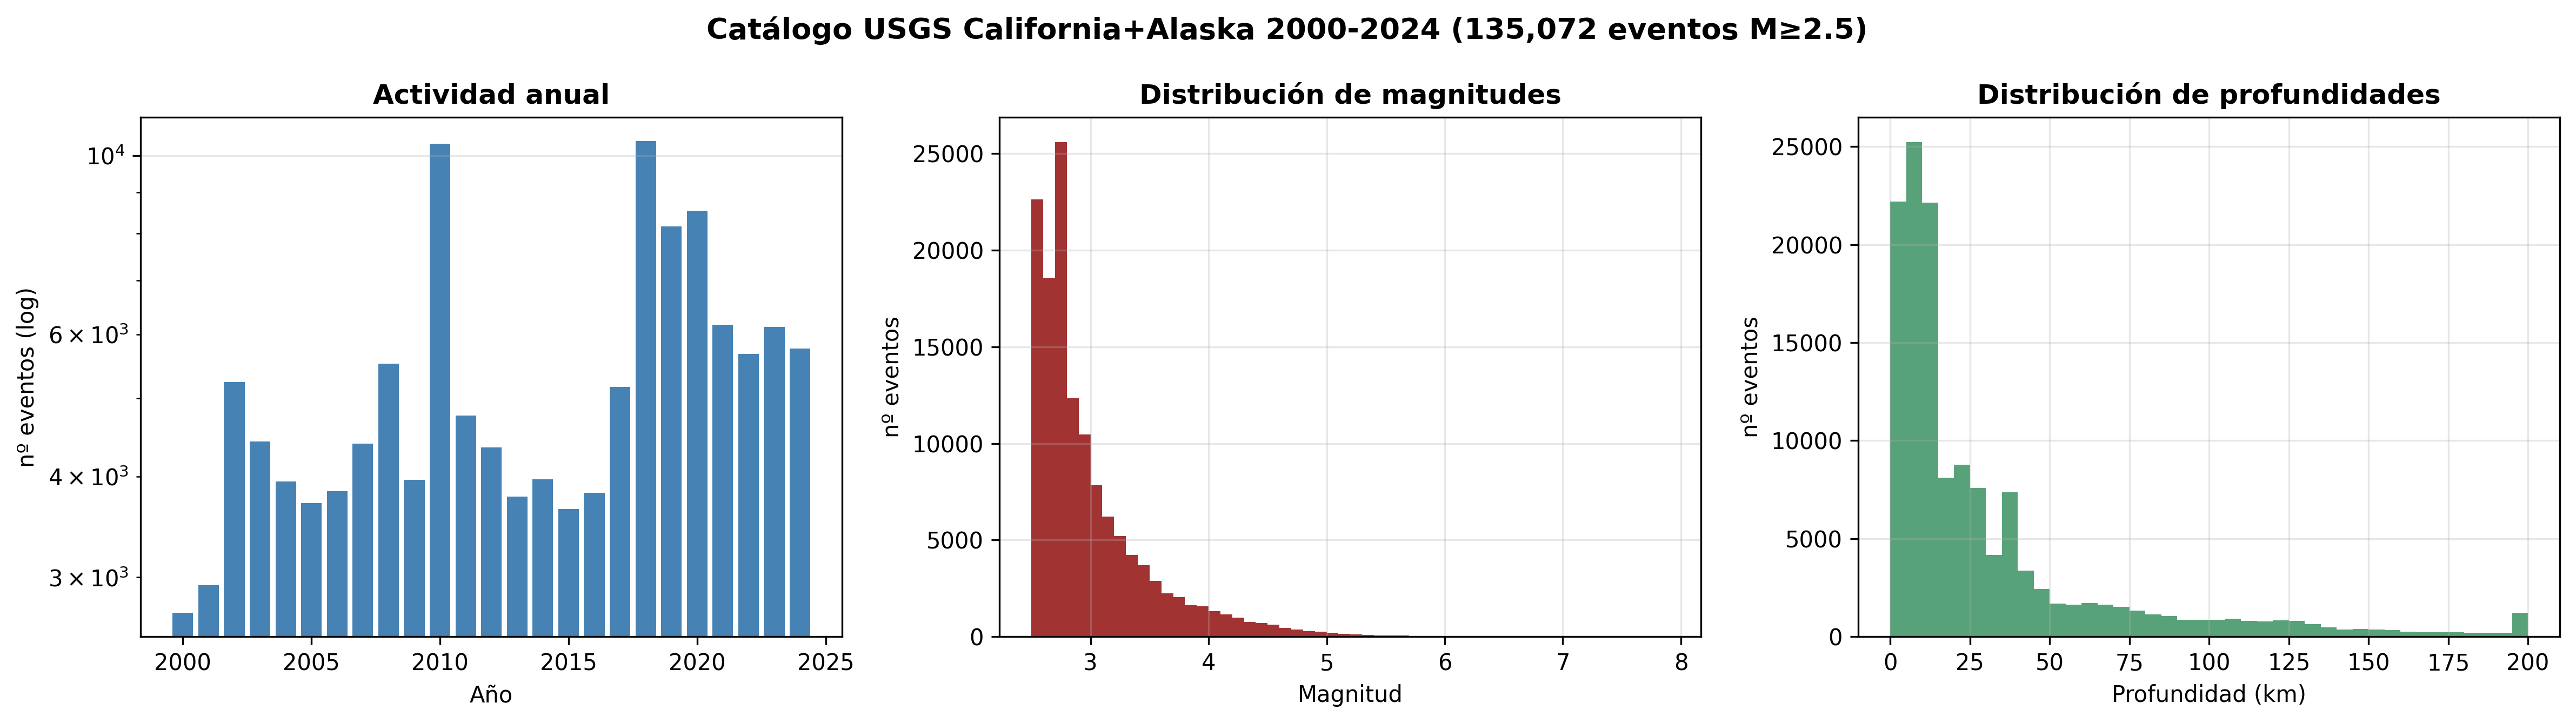
\includegraphics[width=\textwidth]{figuras/03_eda_catalogo}
  \caption[Exploración del catálogo USGS de California y Alaska]{\textbf{Exploración del catálogo USGS (California + Alaska, 2000--2024).} Izquierda: número de eventos por año (escala logarítmica). Centro: distribución de magnitudes. Derecha: distribución de profundidades. El conjunto reúne más de 135.000 eventos de magnitud \(M \geq 2.5\).}
  \label{fig:eda}
\end{figure}

\subsection{Región de estudio y ventana temporal}
\label{md-region}

La región de estudio principal combina dos zonas sísmicamente muy activas y bien
instrumentadas de Estados Unidos: \textbf{California} (\(32^{\circ}\)--\(42^{\circ}\,\)N,
\(-124^{\circ}\)--\(-114^{\circ}\,\)W) y \textbf{Alaska} (\(51^{\circ}\)--\(72^{\circ}\,\)N,
\(-180^{\circ}\)--\(-130^{\circ}\,\)W), en el periodo 2000--2024. La elección responde a
cuatro motivos:

\begin{enumerate}
  \item \textbf{Completitud estable a baja magnitud.} Las redes que cubren ambas zonas
        registran de forma fiable los eventos por encima de \(M_c \approx 2.5\) desde
        mediados de los años noventa. Una magnitud de completitud baja es esencial porque
        las características del modelo se calculan agregando microsismos: si faltaran
        eventos pequeños, esas características estarían sesgadas.
  \item \textbf{Acceso homogéneo.} El catálogo se descarga íntegramente a través del mismo
        \textit{web service}, sin necesidad de combinar fuentes nacionales heterogéneas con
        criterios de catalogación distintos.
  \item \textbf{Más eventos objetivo.} Unir California y Alaska multiplica el número de
        terremotos moderados disponibles para entrenar respecto a usar California sola. Como
        el objetivo del pronóstico son eventos relativamente raros, disponer de más casos
        positivos mejora la robustez estadística del entrenamiento. Conviene matizar este
        punto: aunque California y Alaska responden a regímenes tectónicos distintos, dentro
        de lo que cabe pueden considerarse \emph{compatibles} para entrenar un modelo común.
        Ambas son márgenes muy activos de la placa del Pacífico, con sismicidad
        mayoritariamente somera que sigue la ley de Gutenberg--Richter con \textit{b-values}
        de orden parecido; es decir, las distribuciones estadísticas de sus catálogos --tasas,
        magnitudes, energía-- son lo bastante similares como para que las características
        descritas más adelante tengan el mismo significado en las dos zonas. Esto es lo que
        permite que un mismo modelo aprenda de ambas a la vez sin confundirse.
  \item \textbf{Literatura de referencia abundante.} Ambas regiones están ampliamente
        documentadas, lo que facilita contrastar los valores obtenidos --como el
        \textit{b-value}-- con la literatura y verificar que el preprocesado es correcto.
\end{enumerate}

Conviene señalar que ambas zonas representan regímenes tectónicos distintos: California
está dominada por la falla transformante de San Andrés --donde dos bloques se deslizan
horizontalmente uno respecto al otro-- mientras que Alaska responde a la subducción de la
placa del Pacífico en el arco de las Aleutianas --donde una placa se hunde bajo otra--.
Mantener las dos zonas separadas en el modelado --como se verá en la construcción del grafo
y en la atención del Transformer-- respeta esta diferencia física: el modelo aprende los
patrones \emph{dentro} de cada región sin mezclar geográficamente dos físicas que no tienen
por qué parecerse.

Esta misma observación marca el límite de la estrategia de unir regiones. Podría pensarse en
seguir añadiendo zonas activas --Japón, Chile, el Mediterráneo-- para acumular todavía más
casos positivos, que es el recurso más escaso. Sin embargo, no es aconsejable: cuanto más
heterogéneas son las regiones, más distintas son sus físicas y sus estadísticas, y llega un
punto en que el modelo, que comparte una misma etapa temporal para todas las celdas, ya no
puede aprender una función coherente que sirva para todas a la vez. En otras palabras, el
beneficio de tener más positivos se ve contrarrestado por el ruido de mezclar comportamientos
incompatibles. De hecho, en el desarrollo se probó a ampliar el alcance --incorporando más
fases del catálogo y más regiones-- y el rendimiento no mejoró, lo que confirma de forma
empírica que el equilibrio elegido, dos regiones tectónicamente afines y bien instrumentadas,
es el más adecuado para este trabajo.

\subsection{Magnitud de completitud y declustering}
\label{md-declustering}

Antes de definir el objetivo es necesario tratar dos aspectos del catálogo. El primero es
la \textbf{magnitud de completitud} \(M_c\), el mínimo valor de magnitud a partir del cual
el catálogo se considera completo. En este trabajo se adopta \(M_c = 2.5\), un valor
conservador que asegura completitud incluso en periodos de menor cobertura de la red. Todas
las características se calculan únicamente con eventos por encima de este umbral.

El segundo aspecto, más delicado, es el \textbf{declustering}. Los catálogos sísmicos
contienen secuencias de réplicas que siguen la ley de Omori: tras un terremoto grande
(\textit{mainshock}) llegan numerosos eventos menores cuya tasa decae con el tiempo. Estas
réplicas son altamente predecibles de forma trivial; si no se eliminaran del objetivo,
cualquier modelo aprendería a continuar las secuencias en lugar de a anticipar eventos
nuevos e independientes. Para evitarlo se aplica el algoritmo de Gardner--Knopoff, que para
cada evento candidato a \textit{mainshock} define una ventana espacio-temporal de radio
\(L(M)\)~\eqref{eq:gk-L} y duración \(T(M)\)~\eqref{eq:gk-T} alrededor del evento, y descarta
como dependientes todos los eventos de menor magnitud que caen dentro de ella. El resultado
es un subcatálogo de \emph{mainshocks independientes} sobre el que se define la etiqueta.

Una decisión de diseño central es que el \textit{declustering} se aplica \emph{solo al
  objetivo}, no a las características. El modelo recibe como entrada el catálogo completo
--incluidos los pequeños eventos que podrían contener señal precursora-- y únicamente el
conjunto de mainshocks que define la etiqueta pasa por el filtro. De este modo se purifica
la variable que se quiere predecir sin sacrificar la información de entrada. Esta asimetría
es coherente con la práctica recomendada en la literatura y, como se verá en los estudios
de ablación (Sección~\ref{res-ablations}), resulta metodológicamente necesaria: si no se
declusteriza, el rendimiento aparente sube, pero solo a costa de aprender la
predictibilidad trivial de las réplicas.

\subsection{Definición del objetivo}
\label{md-target}

El objetivo del pronóstico se plantea como un problema binario sobre una ventana de
\textbf{30 días}. En la formulación espacial, para cada celda \(c\) y cada día \(t\) la
etiqueta vale 1 si en los siguientes 30 días ocurre al menos un mainshock independiente de
magnitud \(M \geq 4.5\) relacionado con la celda, y 0 en caso contrario. El umbral
\(M \geq 4.5\) equilibra tres criterios. Primero, un \textbf{volumen suficiente}: por
debajo de \(4.5\) habría demasiados eventos poco relevantes, y por encima de \(5.0\)
quedarían muy pocos casos positivos para entrenar. Segundo, la \textbf{relevancia
  operativa}: un sismo de \(M \geq 4.5\) ya es potencialmente dañino en entornos urbanos
vulnerables. Tercero, la \textbf{homogeneidad del catálogo}: con \(M_c = 2.5\) y un
objetivo en \(4.5\), la distancia de dos unidades de magnitud asegura que el catálogo es
completo tanto para las características como para el objetivo.

En los modelos espaciales, la etiqueta de una celda se calcula además con una
\textbf{expansión 3\(\times\)3}: vale 1 si el mainshock cae en la propia celda o en
cualquiera de sus ocho vecinas inmediatas, lo que equivale a un radio efectivo de unos
55\,km. Esta expansión tiene tres justificaciones. Tiene sentido físico --interesa saber si
habrá un terremoto \emph{cerca}, no en una celda exacta--; absorbe el error de localización
del catálogo, que es de varios kilómetros; y evita que la proporción de positivos por celda
baje a niveles que impidan el aprendizaje. Aun con la expansión, el problema es fuertemente
desbalanceado, como se discute en la Sección~\ref{planteamiento-del-problema}.

\subsection{Ingeniería de características}
\label{md-features}

Antes de calcular las características se discretiza la región en una rejilla regular de
celdas de \(0.5^{\circ} \times 0.5^{\circ}\), aproximadamente 50\,km de lado. Cada
evento se asigna a la celda que lo contiene. Se conservan únicamente las \emph{celdas
  activas}, definidas como aquellas con al menos 30 eventos en todo el periodo; las celdas con
muy poca actividad aportan más ruido que señal y se descartan para evitar la maldición de la
dimensionalidad. La Figura~\ref{fig:grid} muestra la rejilla resultante: la sismicidad se
concentra claramente a lo largo de las grandes estructuras tectónicas.

\begin{figure}[ht!]
  \centering
  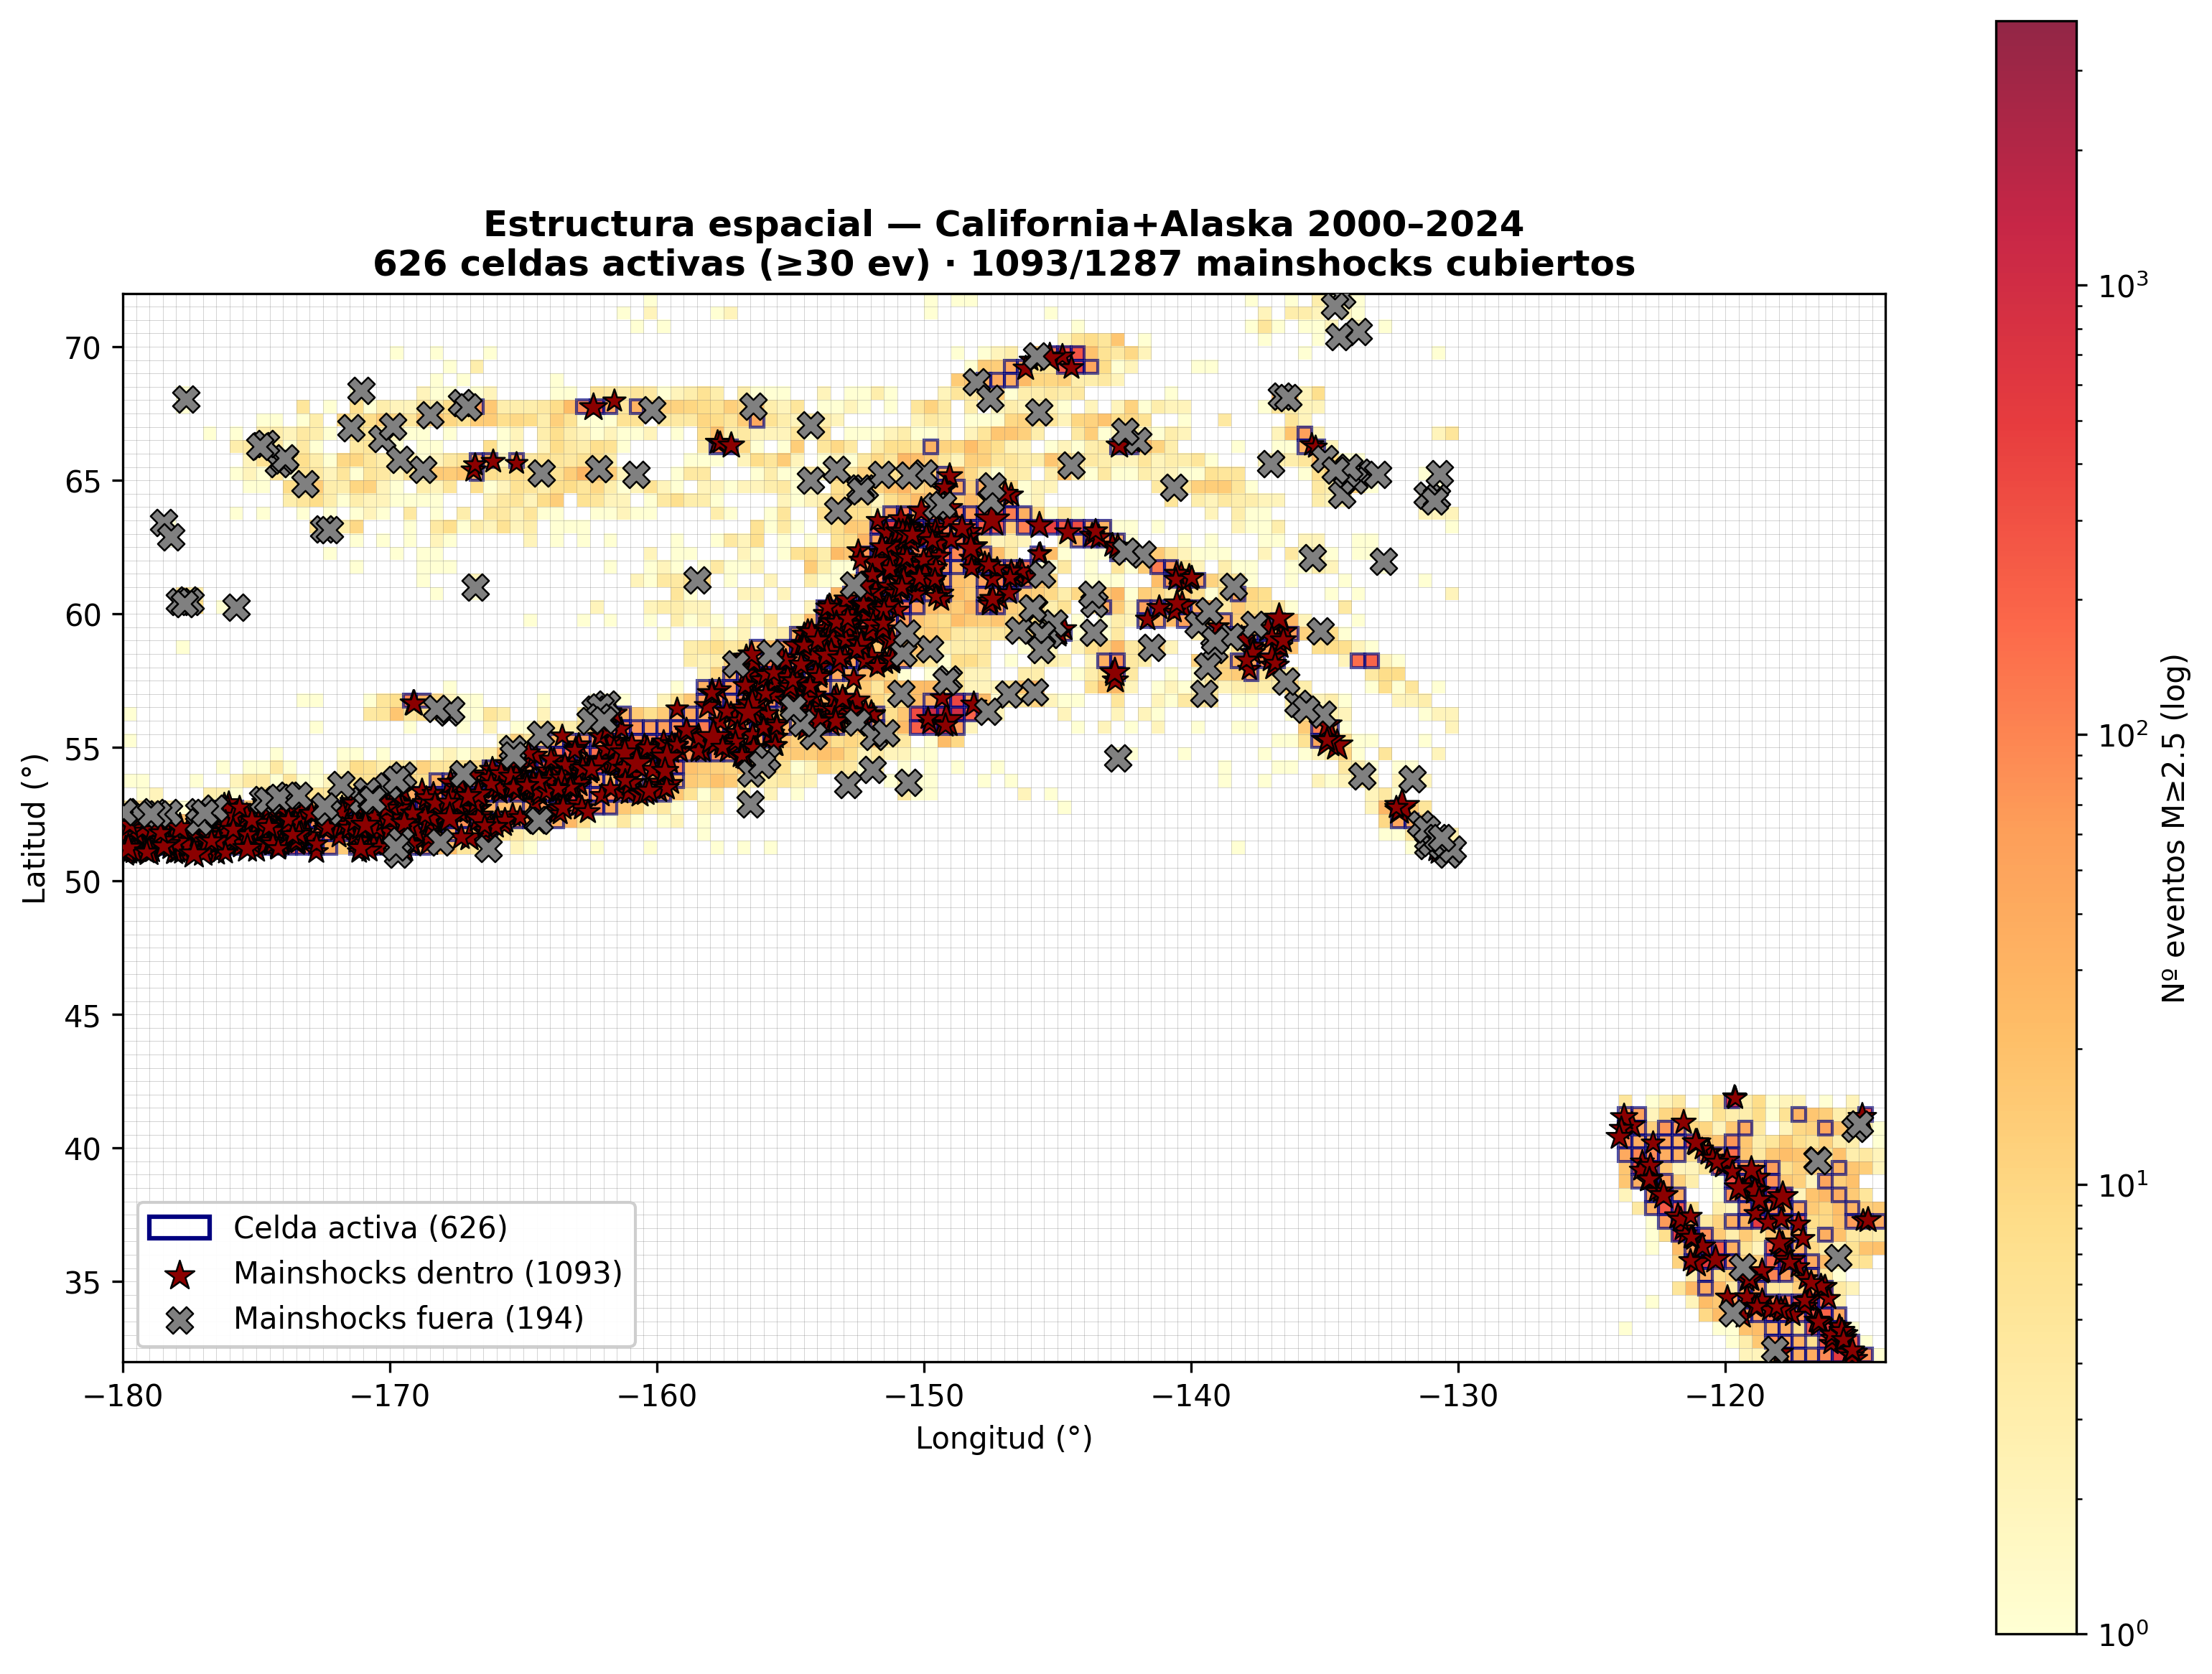
\includegraphics[width=0.92\textwidth]{figuras/05_grid_espacial_M4.5_min30}
  \caption[Discretización espacial en celdas y celdas activas]{\textbf{Discretización espacial de la región de estudio.} Cada evento se asigna a una celda de \(0.5^{\circ}\times 0.5^{\circ}\); se conservan las celdas con al menos 30 eventos (celdas activas). La sismicidad se alinea con la falla de San Andrés en California y con el arco de las Aleutianas en Alaska.}
  \label{fig:grid}
\end{figure}

Para cada celda activa y cada día se calculan cinco características, pensadas para capturar
distintos aspectos de la actividad sísmica:

\begin{enumerate}
  \item \textbf{Recuento logarítmico} de eventos del día, \(\log(1+n)\), donde \(n\) es el
        número de eventos con \(M \geq M_c\). La transformación logarítmica comprime el
        rango dinámico, ya que un evento grande puede generar miles de réplicas en un solo
        día y desestabilizaría el entrenamiento sin esta compresión.
  \item \textbf{Energía logarítmica} liberada, \(\log(1+E)\), donde la energía \(E\) se
        obtiene de la magnitud mediante la relación~\eqref{eq:kanamori}. Esta característica
        pondera los eventos por su tamaño y no solo por su número.
  \item \textbf{Magnitud máxima} registrada en la celda ese día, que destaca la presencia de
        eventos moderados.
  \item \textbf{Recuento de eventos moderados} (\(M \geq 3.5\)) en escala logarítmica, que
        aísla la actividad más energética del ruido de microsismos.
  \item \textbf{\textit{b-value} móvil} de 30 días, estimado por máxima verosimilitud con el
        estimador de Aki~\eqref{eq:b-aki}. El \textit{b-value} resume la proporción entre
        sismos pequeños y grandes y tiene significado físico: descensos transitorios se
        asocian a un mayor estado de estrés. Se calcula por región y no por celda, porque su
        estimación necesita decenas de eventos para ser estable, y se asigna a cada celda el
        valor de su región.
\end{enumerate}

Otras características también se probaron en varios experimentos sin que mejoraran el modelo,
por lo que finalmente se descartaron y no forman parte del conjunto definitivo. La primera fue
la \textbf{profundidad} de los terremotos: se añadió un sexto canal con la profundidad media de
los seísmos de cada celda y día --en una variante, ponderada por la energía de los eventos, de
modo que un terremoto grande y profundo pesara más que un microsismo somero--, con la idea de
que la profundidad ayuda a distinguir regímenes sísmicos distintos, como los eventos profundos
de la subducción de Alaska frente a los corticales someros. Sin embargo, la profundidad media
diaria resultó muy volátil y, lejos de ayudar, redujo ligeramente el rendimiento; una posible
explicación es que su información ya está parcialmente recogida de forma implícita por la
energía. La segunda familia de características ensayada fueron \textbf{indicadores de anomalía
  de la tasa sísmica} por celda --que comparan la actividad reciente en una ventana corta con su
línea base en una ventana larga-- pensados para captar aceleraciones o silencios sísmicos que
la literatura asocia a posibles precursores; tampoco aportaron señal apreciable. En total se
llegó a tantear hasta ocho canales, pero ninguna de estas adiciones superó a las cinco
características originales.

La Tabla~\ref{tab:features} resume las cinco características, su transformación y la dimensión
del fenómeno que cada una pretende capturar. En conjunto cubren tres aspectos complementarios
de la sismicidad: \emph{cuánta} actividad hay (recuentos), \emph{cómo de energética} es
(energía y magnitud máxima) y \emph{cómo se reparte} entre tamaños (\textit{b-value}). Esta
diversidad busca dar al modelo una visión completa del estado de cada celda con un número
reducido de variables, lo que es deseable dado el tamaño limitado del conjunto de datos.

\begin{table}[ht!]
  \centering
  \small
  \begin{tabular}{@{}llll@{}}
    \toprule
    \textbf{\#} & \textbf{Característica}  & \textbf{Transformación} & \textbf{Captura}     \\
    \midrule
    1           & Recuento de eventos      & $\log(1+n)$             & volumen de actividad \\
    2           & Energía liberada         & $\log(1+E)$             & energía total        \\
    3           & Magnitud máxima          & valor directo           & eventos destacados   \\
    4           & Recuento $M\geq 3.5$     & $\log(1+n_{3.5})$       & actividad energética \\
    5           & \textit{b-value} (30\,d) & estimador de Aki        & reparto por tamaños  \\
    \bottomrule
  \end{tabular}
  \caption[Características de entrada de los modelos de pronóstico]{\textbf{Características de entrada.} Las cinco variables calculadas por celda y día, con su transformación y el aspecto de la sismicidad que capturan. Todas se calculan de forma causal sobre eventos $M\geq M_c$.}
  \label{tab:features}
\end{table}

Dos cuidados son esenciales para la validez del experimento. Primero, todas las
características se calculan de forma \emph{causal}: cada valor en el día \(t\) usa únicamente
información hasta ese día, de modo que en ningún momento entra información del futuro.
Segundo, la normalización a media cero y desviación uno se ajusta exclusivamente sobre el
conjunto de entrenamiento, y las mismas medias y desviaciones se aplican después a
validación y test, evitando así cualquier fuga de información entre particiones.

El Algoritmo~\ref{alg:dataset} resume el procedimiento completo de construcción del conjunto
de datos espacio-temporal, desde el catálogo bruto hasta los tensores de entrada y las
etiquetas que reciben los modelos. Su lectura permite verificar, paso a paso, que la
causalidad y la separación entre características y objetivo se respetan en todo momento.

\begin{algorithm}[ht!]
  \caption{Construcción del conjunto de datos espacio-temporal}
  \label{alg:dataset}
  \DontPrintSemicolon
  \KwIn{Catálogo de eventos $\mathcal{C}$; magnitud de completitud $M_c$; umbral objetivo $M_t=4.5$; ventana de historia $L=60$; ventana de predicción $T=30$.}
  \KwOut{Tensor de características $X$, matriz de etiquetas $Y$, grafo $G$.}
  Discretizar la región en celdas de $0.5^{\circ}\times 0.5^{\circ}$ y asignar cada evento a su celda\;
  Conservar las celdas con $\geq 30$ eventos (celdas activas)\;
  Construir el grafo $G$ uniendo celdas a $<100$\,km dentro de cada región\;
  Obtener el subcatálogo de mainshocks independientes con Gardner--Knopoff\;
  \For{cada celda activa $c$}{
    \For{cada día $t$}{
      Calcular las 5 características causales con eventos $M\geq M_c$ hasta $t$\;
      $Y[c,t] \leftarrow 1$ si hay un mainshock $M\geq M_t$ en $c$ o sus vecinas en $[t+1,t+T]$; si no, $0$\;
    }
  }
  Particionar en train (2000--2020), validación (2021--2022) y test (2023--2024)\;
  Ajustar la normalización en train y aplicarla a las tres particiones\;
  \Return $X$, $Y$, $G$\;
\end{algorithm}

\subsection{Construcción del grafo espacial}
\label{md-grafo}

Los modelos espaciales necesitan una noción de vecindad entre celdas. Esta se representa
como un grafo \(G=(V,E)\) en el que cada celda activa es un nodo y existe una arista entre
dos celdas si su distancia, medida con la fórmula de Haversine~\eqref{eq:haversine}, es
menor que 100\,km. Para garantizar que ninguna celda quede aislada --lo que dejaría sus
características estancadas en la propagación-- se añade además una conexión a las dos vecinas
más cercanas aunque superen el umbral. Como California y Alaska están separadas por más de
3.000\,km, las aristas se restringen al interior de cada región: el grafo final tiene dos
componentes conexas, una por zona, y el modelo opera sobre ambas a la vez. La
Figura~\ref{fig:grafo} muestra el grafo sobre el mapa.

\begin{figure}[ht!]
  \centering
  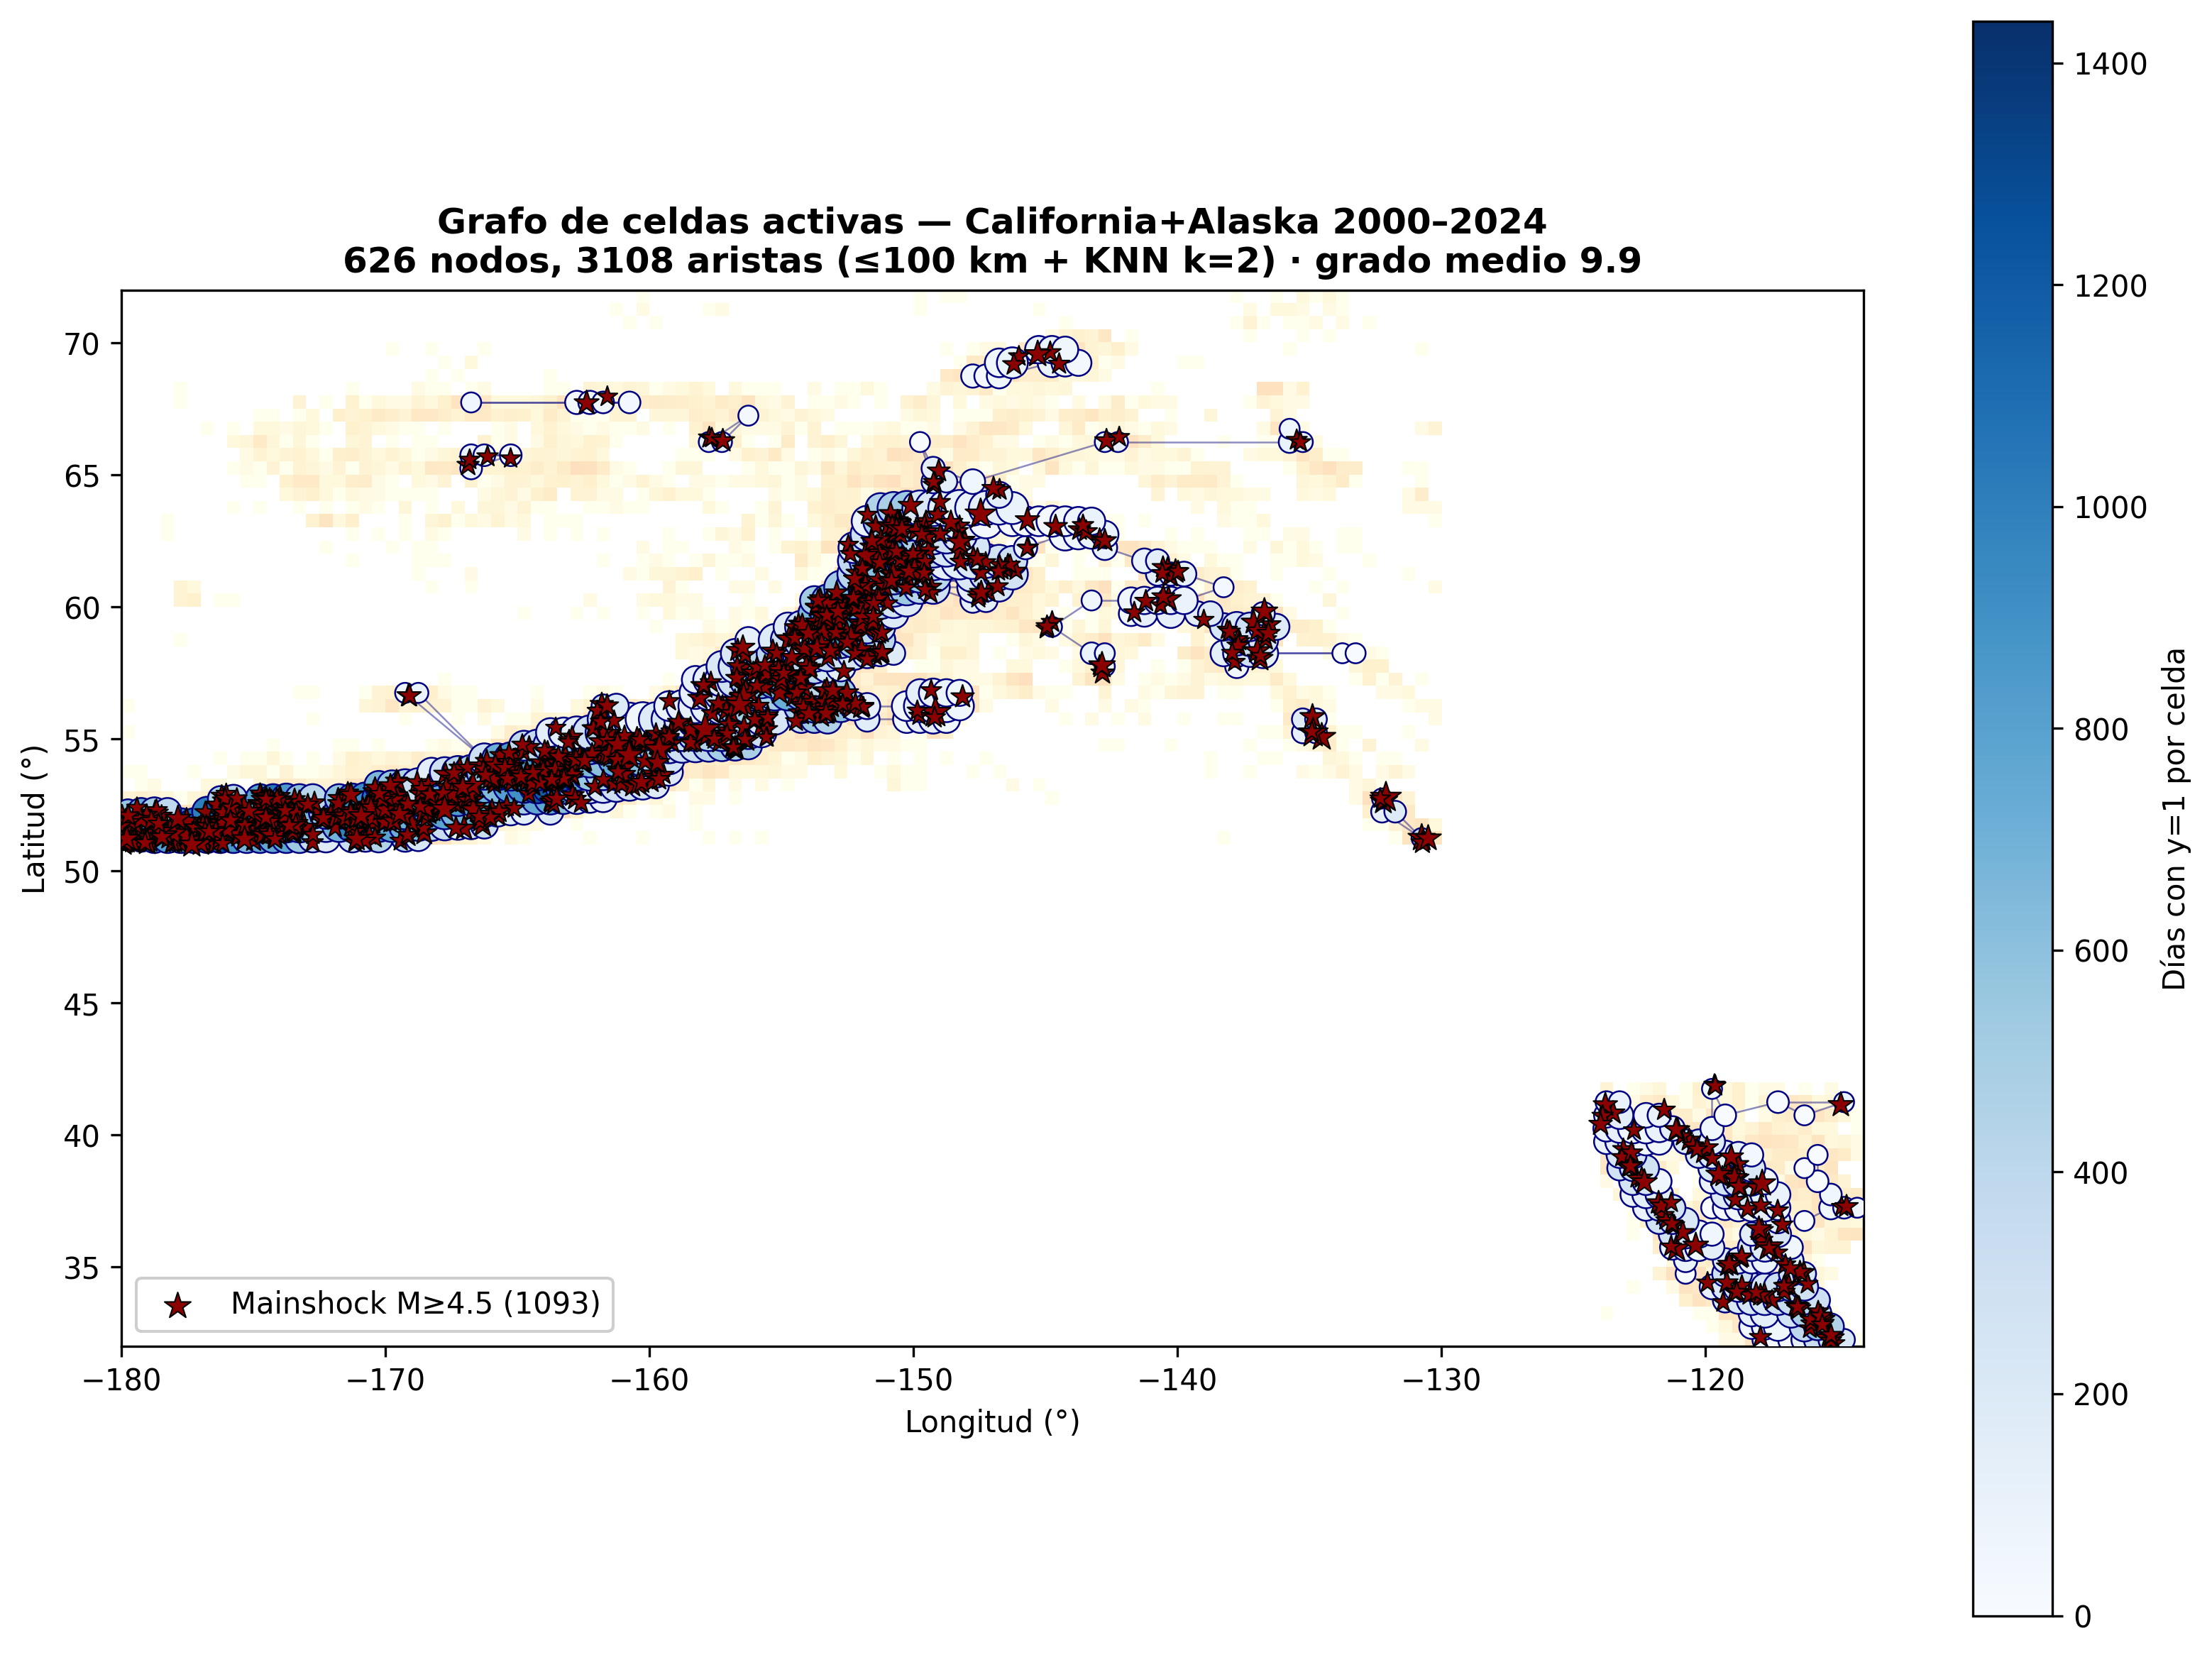
\includegraphics[width=0.92\textwidth]{figuras/05_grafo_celdas_d100km}
  \caption[Grafo de vecindad entre celdas activas]{\textbf{Grafo de vecindad espacial.} Los nodos son las celdas activas y las aristas conectan celdas a menos de 100\,km dentro de la misma región. La estructura reproduce los grandes alineamientos tectónicos y mantiene separadas las dos zonas de estudio.}
  \label{fig:grafo}
\end{figure}

\subsection{Particiones temporales}
\label{md-splits}

Para evitar que el modelo ``vea el futuro'' durante el entrenamiento, las particiones son
estrictamente temporales, no aleatorias. El conjunto de \textbf{entrenamiento} abarca de
2000 a 2020, el de \textbf{validación} 2021--2022 --usado para la parada temprana y la
selección de hiperparámetros-- y el de \textbf{test} 2023--2024, reservado por completo para
la evaluación final. Este esquema reproduce las condiciones reales de un sistema de
pronóstico: en cada instante solo se dispone del pasado. Conviene notar que el historial de
60 días que mira el modelo para predecir el primer día de test procede del final del periodo
de validación; esto no constituye fuga de información, ya que se trata de datos de entrada
(el pasado observable) y nunca de las etiquetas de test, que permanecen intactas durante todo
el desarrollo.

\subsection{Arquitecturas de los modelos}
\label{md-arquitecturas}

Esta sección describe en detalle las cuatro arquitecturas que componen el \textit{pipeline}
de pronóstico y cartografía. Todas comparten un mismo bloque temporal --una red convolucional
temporal-- y se diferencian en cómo tratan la dimensión espacial.

\subsubsection{Red convolucional temporal (TCN)}
\label{md-arq-tcn}

La TCN es el bloque que procesa la evolución temporal de las características. Sustituye la
recurrencia de las redes recurrentes clásicas por una pila de convoluciones unidimensionales
con tres propiedades. Son \emph{causales}, es decir, la salida en el instante \(t\) depende
solo de las entradas en instantes \(t' \leq t\), lo que se logra desplazando la convolución
para no usar el futuro. Son \emph{dilatadas}: la capa \(\ell\)-ésima usa una dilatación
\(d_\ell = 2^{\ell-1}\), de modo que el campo receptivo crece exponencialmente con la
profundidad según la relación~\eqref{eq:rf-tcn}. Y emplean \emph{bloques residuales}, en los
que cada bloque suma su entrada a su salida, lo que facilita el entrenamiento de redes
profundas.

Cada \textbf{bloque residual} contiene dos convoluciones causales dilatadas, cada una seguida
de una normalización, una función de activación no lineal y una capa de \textit{dropout}; la
entrada del bloque se suma a su salida mediante una conexión de atajo (cuando las dimensiones
no coinciden, la conexión incluye una convolución \(1\times 1\) que las ajusta). Esta suma
residual es la que permite que el gradiente fluya sin atenuarse a través de muchas capas, de
modo que la red profunda se entrena con estabilidad. Formalmente, si \(\mathbf{x}\) es la
entrada del bloque y \(\mathcal{F}\) la transformación de sus dos convoluciones, la salida es
\(\mathbf{y} = \text{act}(\mathbf{x} + \mathcal{F}(\mathbf{x}))\).

En la configuración utilizada, la pila tiene tres niveles con dilataciones \(\{1,2,4\}\) y
canales \((32, 32, 64)\), o cuatro niveles con dilataciones \(\{1,2,4,8\}\) en la variante
global del notebook de pronóstico temporal. El tamaño de \textit{kernel} es \(k=3\). Aplicando
la relación~\eqref{eq:rf-tcn}, el campo receptivo de la variante de cuatro niveles abarca
\(1 + 2\,(k-1)\sum_{\ell} d_\ell = 1 + 2\cdot 2\cdot(1{+}2{+}4{+}8) = 61\) días, justo lo
necesario para cubrir la ventana de historia de 60 días sin desperdiciar capacidad. Esta es la
ventaja esencial de las dilataciones: alcanzar un horizonte temporal amplio con muy pocas capas
y, por tanto, con pocos parámetros.

La cabeza de clasificación no se limita al último instante temporal, sino que concatena tres
estadísticos de la secuencia de salida: el estado final causal, la media y el máximo a lo largo
del tiempo. Esto da al modelo acceso explícito tanto al ``presente'' (el último día) como a
estadísticos globales de toda la ventana, lo que mejora la sensibilidad a patrones distribuidos
en el tiempo, como un aumento sostenido de la actividad. En el modelo temporal global, la salida
es un único logit; en los modelos espaciales, la TCN se aplica de forma compartida a cada celda,
produciendo un vector de características por celda que alimenta la etapa espacial.

El Algoritmo~\ref{alg:tcn} resume el paso hacia delante de la TCN, desde la ventana de historia
hasta la representación que usa la cabeza de clasificación. Es el bloque base del sistema: en la
Fase 2 produce directamente un \textit{logit}, y en las Fases 3 y 4 se reutiliza, con los mismos
pesos, para resumir la historia de cada celda antes de la etapa espacial.

\begin{algorithm}[ht!]
  \caption{Paso hacia delante de la red convolucional temporal (TCN)}
  \label{alg:tcn}
  \DontPrintSemicolon
  \KwIn{Serie de características $X \in \mathbb{R}^{L\times F}$ (ventana de $L=60$ días, $F=5$ características); dilataciones $\{d_1,\dots,d_B\}=\{1,2,4,8\}$.}
  \KwOut{\textit{Logit} de riesgo (Fase 2) o vector de características (Fases 3--4).}
  $h \leftarrow X$\;
  \For{cada bloque residual $b = 1,\dots,B$}{
    $z \leftarrow \text{ConvCausalDilatada}_{d_b}(h)$ \tcp*{2 convoluciones, \textit{kernel} 3}
    $z \leftarrow \text{Dropout}(\text{act}(\text{Norm}(z)))$\;
    $h \leftarrow \text{act}\big(h + z\big)$ \tcp*{suma residual (atajo $1{\times}1$ si hace falta)}
  }
  $e \leftarrow [\,h^{\text{final}} \,\|\, \overline{h} \,\|\, \max h\,]$ \tcp*{\textit{pooling} temporal}
  \eIf{modelo temporal global (Fase 2)}{
    \Return $w^\top e + b$ \tcp*{un único \textit{logit}}
  }{
    \Return $e$ \tcp*{vector de características de la celda}
  }
\end{algorithm}

\subsubsection{Red neuronal de grafos (GNN)}
\label{md-arq-gnn}

La GNN es el primer modelo que incorpora la dimensión espacial. Su arquitectura,
denominada \textit{SpatioTemporalGNN}, combina dos bloques. En primer lugar, una \textbf{TCN
  compartida} procesa la serie temporal de cada celda de forma independiente, con los mismos
pesos para todas las celdas (\textit{weight sharing}); el resultado es un vector de
características o \textit{embedding} por celda, que resume su historia reciente. En segundo
lugar, \textbf{dos capas convolucionales de grafo} (GCN) propagan información entre celdas
vecinas.

Cada capa GCN aplica la operación~\eqref{eq:gcn}, que en su forma matricial se escribe
\(H^{(l+1)} = \sigma\!\big(\tilde{D}^{-1/2}\tilde{A}\,\tilde{D}^{-1/2} H^{(l)} W^{(l)}\big)\),
donde \(\tilde{A} = A + I\) es la matriz de adyacencia con bucles propios añadidos --para que
cada celda tenga en cuenta también su propia información--, \(\tilde{D}\) es su matriz de
grados y \(W^{(l)}\) es la matriz de pesos aprendible de la capa. La normalización simétrica
\(\tilde{D}^{-1/2}\tilde{A}\,\tilde{D}^{-1/2}\) evita que las celdas con muchos vecinos
dominen la propagación, equilibrando la contribución de cada nodo. Intuitivamente, cada capa
sustituye el vector de una celda por una media ponderada de los vectores de sus vecinas (y el
suyo propio), seguida de una transformación lineal y una no linealidad. Apilando dos capas,
cada celda recibe información de su entorno a dos saltos de distancia. Una cabeza lineal por
nodo produce finalmente un logit por celda.

El uso de pesos compartidos en la TCN y de matrices de adyacencia precomputadas mantiene el
número de parámetros moderado, en torno a las decenas de miles, lo que es adecuado para un
conjunto de datos de tamaño limitado. Es importante subrayar que el modelo no memoriza celdas
concretas: aprende una \emph{función} de las características y de la estructura de vecindad,
lo que en principio permitiría aplicarlo a otras regiones sin reentrenar desde cero.

\subsubsection{Transformer geoespacial}
\label{md-arq-transformer}

El Transformer geoespacial explora una segunda forma de modelar el espacio. Mantiene el mismo
procesamiento temporal por celda mediante una TCN compartida, pero sustituye la propagación
por grafo por un mecanismo de \textbf{atención}. En lugar de imponer de antemano qué celdas
son vecinas, la atención~\eqref{eq:attention} permite que el modelo aprenda, para cada
predicción, qué celdas son relevantes, ponderando la contribución de cada una.

El mecanismo funciona del siguiente modo. El \textit{embedding} de cada celda se proyecta en
tres vectores: una \emph{consulta} (\textit{query}), una \emph{clave} (\textit{key}) y un
\emph{valor} (\textit{value}). La relevancia de la celda \(j\) para la celda \(i\) se calcula
como el producto escalar entre la consulta de \(i\) y la clave de \(j\), escalado por la raíz
de la dimensión y normalizado con una función \textit{softmax} sobre todas las celdas; el
nuevo vector de la celda \(i\) es entonces la media de los valores, ponderada por esas
relevancias. Este cómputo se realiza en paralelo en \textbf{cuatro cabezas} de atención, cada
una con sus propias proyecciones, lo que permite al modelo atender simultáneamente a distintos
tipos de relación espacial; las salidas de las cuatro cabezas se concatenan y se combinan. La
posición geográfica de cada celda se inyecta mediante una \textbf{codificación posicional
  sinusoidal} de sus coordenadas, análoga a la usada en el procesamiento de lenguaje pero
adaptada a coordenadas continuas: la mitad de las dimensiones codifican la latitud y la otra
mitad la longitud, mediante senos y cosenos a frecuencias geométricamente espaciadas, de modo
que celdas próximas reciben codificaciones parecidas y el modelo puede inferir distancias.

La configuración emplea una dimensión de \textit{embedding} de 128, cuatro cabezas de
atención y dos capas de codificador, cada una con su bloque de atención y su red
\textit{feed-forward}, conectadas por sumas residuales y normalización. Para respetar la
separación tectónica entre California y Alaska, la atención se restringe mediante una máscara
que asigna relevancia nula (un valor \(-\infty\) antes de la \textit{softmax}) a los pares de
celdas de regiones distintas: cada celda solo presta atención a las de su propia región. Esta
variante enmascarada es la que mejor rendimiento ofrece y la que alimenta la fase de
cartografía. Una cabeza lineal por celda produce el logit final.

Pese a sus diferencias, la GNN y el Transformer comparten el mismo esqueleto de cómputo, que
el Algoritmo~\ref{alg:forward} hace explícito: una etapa temporal idéntica, compartida entre
todas las celdas, seguida de una etapa de mezcla espacial que es lo único que distingue a
ambos modelos. Esta estructura común es precisamente lo que permite atribuir las diferencias
de rendimiento al mecanismo espacial y no al procesamiento temporal.

\begin{algorithm}[ht!]
  \caption{Paso hacia delante de los modelos espaciales (GNN / Transformer)}
  \label{alg:forward}
  \DontPrintSemicolon
  \KwIn{Ventana de características $X \in \mathbb{R}^{N\times L\times 5}$ ($N$ celdas, $L$ días); grafo $G$ (GNN) o coordenadas $(\text{lat},\text{lon})$ (Transformer).}
  \KwOut{Logits de riesgo $z \in \mathbb{R}^{N}$ (uno por celda).}
  \For{cada celda $c \in \{1,\dots,N\}$}{
    $e_c \leftarrow \text{TCN}_\theta(X_c)$ \tcp*{Algoritmo~\ref{alg:tcn}, misma $\theta$ para todas las celdas}
  }
  $E \leftarrow [e_1,\dots,e_N]$ \tcp*{matriz de \textit{embeddings} de celda}
  \eIf{modelo $=$ GNN}{
    \For{cada capa $\ell = 1, 2$}{
      $E \leftarrow \sigma\big(\tilde{D}^{-1/2}\tilde{A}\,\tilde{D}^{-1/2}\, E\, W^{(\ell)}\big)$ \tcp*{GCN: media sobre vecinos del grafo}
    }
  }{
    $E \leftarrow E + \text{PosEnc}(\text{lat},\text{lon})$ \tcp*{codificación geográfica}
    \For{cada capa $\ell = 1, 2$}{
      $E \leftarrow \text{AtenciónMultiCabeza}_{\text{enmasc.}}(E)$ \tcp*{cada celda atiende a las de su región}
    }
  }
  \For{cada celda $c$}{ $z_c \leftarrow w^\top E_c + b$ \tcp*{cabeza lineal por celda} }
  \Return $z$\;
\end{algorithm}

\subsubsection{Proceso Gaussiano para la cartografía del riesgo}
\label{md-arq-gp}

La última arquitectura no es una red neuronal, sino un \textbf{proceso gaussiano} (GP), un
método bayesiano no paramétrico ideal para interpolar con incertidumbre. Un GP define una
distribución de probabilidad sobre funciones, caracterizada por una función de media y una
función de covarianza o \textit{kernel} \(k(\mathbf{x},\mathbf{x}')\), que codifica cómo de
parecidos se espera que sean los valores de la función en dos puntos según su distancia. Dadas
unas observaciones --en este caso, las probabilidades de riesgo calibradas en los centroides de
las celdas activas-- el GP produce, para cualquier punto \(\mathbf{x}_*\) del mapa, una
predicción que es a su vez una distribución gaussiana. Su media es
\(\mu_* = \mathbf{k}_*^\top (K + \sigma^2 I)^{-1}\mathbf{y}\) --una media ponderada de las
observaciones, donde el peso de cada una decae con la distancia-- y su varianza es
\(\sigma_*^2 = k(\mathbf{x}_*,\mathbf{x}_*) - \mathbf{k}_*^\top (K + \sigma^2 I)^{-1}\mathbf{k}_*\),
que crece a medida que el punto se aleja de las observaciones. De ahí que el GP entregue de
forma natural, y sin coste adicional, el mapa de incertidumbre junto al de riesgo.

Se emplea un \textit{kernel} de tipo Matérn, habitual en datos espaciales porque genera
superficies suaves pero no excesivamente regulares, más realistas para un fenómeno físico que el
\textit{kernel} gaussiano. El parámetro de suavidad \(\nu\) del Matérn controla cuántas veces es
diferenciable la superficie resultante; valores intermedios (como \(\nu = 3/2\)) producen mapas
con un grado de rugosidad coherente con la distribución real de la sismicidad. Los parámetros del
\textit{kernel} --la escala de longitud y la varianza-- se ajustan por máxima verosimilitud sobre
las propias observaciones. El GP se ajusta por separado en cada región, ya que interpolar a
través de los 3.000\,km que separan California y Alaska no tendría ningún sentido físico.

\subsection{Función de pérdida y manejo del desbalance}
\label{md-loss}

El pronóstico sísmico es un problema fuertemente desbalanceado: en la formulación por celda,
solo en torno al 4.5\,\% de los pares (celda, día) son positivos. Si no se corrige, un
modelo entrenado con la entropía cruzada habitual tendería a predecir siempre ``no habrá
terremoto'', que es correcto la mayor parte del tiempo pero inútil. Para evitarlo se utiliza
una entropía cruzada binaria con \emph{ponderación de clase}, que asigna a los ejemplos
positivos un peso proporcional a su escasez, de modo que el modelo no pueda ignorarlos. En
algunas variantes se emplea además una \emph{pérdida focal}, que reduce automáticamente el
peso de los ejemplos fáciles de clasificar y concentra el aprendizaje en los difíciles. Estas
elecciones permiten que el entrenamiento atienda a la clase minoritaria sin necesidad de
sobremuestrearla.

\subsection{Optimización, entrenamiento y reproducibilidad}
\label{md-optim}

Todos los modelos se entrenan con el optimizador Adam, con una tasa de aprendizaje inicial
del orden de \(10^{-4}\)--\(10^{-3}\), regularización \(L_2\) sobre los pesos y
\textit{dropout} para evitar el sobreajuste, especialmente importante dado el tamaño limitado
del conjunto de datos. Se emplea además un planificador que reduce la tasa de aprendizaje
cuando la métrica de validación deja de mejorar, y una parada temprana que detiene el
entrenamiento y recupera el mejor punto cuando la validación no progresa durante un número
fijo de épocas. La Tabla~\ref{tab:hiperparametros} reúne los hiperparámetros más relevantes
del sistema; el detalle completo, separado en hiperparámetros de \emph{arquitectura} y de
\emph{entrenamiento} para cada uno de los tres modelos, se recoge en las
Tablas~\ref{tab:hiper-arq} y~\ref{tab:hiper-train} del Apéndice~\ref{apendice-i}.

\begin{table}[ht!]
  \centering
  \small
  \begin{tabular}{@{}ll@{}}
    \toprule
    \textbf{Hiperparámetro}                 & \textbf{Valor}                               \\
    \midrule
    Ventana de historia (\textit{lookback}) & 60 días                                      \\
    Ventana de predicción                   & 14 días (TCN) / 30 días (modelos espaciales) \\
    Tamaño de \textit{kernel} de la TCN     & 3                                            \\
    Dim.\ de mezcla espacial                & 64 (GNN, GCN) / 128 (Transformer, atención)  \\
    Optimizador                             & Adam                                         \\
    Tasa de aprendizaje                     & $10^{-4}$--$10^{-3}$                         \\
    \textit{Dropout}                        & 0.15--0.20                                   \\
    Parada temprana                         & sí (paciencia 6--12 épocas)                  \\
    \bottomrule
  \end{tabular}
  \caption[Hiperparámetros más relevantes del sistema]{\textbf{Hiperparámetros más relevantes} del sistema. El detalle completo por modelo, separado en arquitectura y entrenamiento, figura en el Apéndice~\ref{apendice-i}.}
  \label{tab:hiperparametros}
\end{table}

Para garantizar la reproducibilidad, todas las semillas aleatorias están fijadas, el código
se conserva en un repositorio con control de versiones y el catálogo se almacena en formato
estable. El conjunto de test no interviene en ningún momento del desarrollo.

\subsection{Métricas de evaluación}
\label{md-metricas}

La evaluación es deliberadamente exigente, porque en un problema tan desbalanceado las
métricas habituales pueden inducir a error. Se emplean las siguientes:

\begin{itemize}
  \item \textbf{AUC-ROC.} Mide la probabilidad de que el modelo asigne mayor riesgo a un caso
        positivo que a uno negativo, ambos tomados al azar. Es la métrica principal por su
        robustez al desbalance y porque no depende de la elección de un umbral.
  \item \textbf{PR-AUC.} Área bajo la curva \textit{precision}-\textit{recall}, más informativa
        que la ROC cuando la clase positiva es muy minoritaria, porque ignora los abundantes
        verdaderos negativos.
  \item \textbf{\textit{Precision}, \textit{recall} y \textit{lift} en el top \(K\).} Traducen
        el modelo a un sistema de alerta a partir de la definición~\eqref{eq:precision-recall}:
        si solo se puede alertar de un porcentaje pequeño de las ventanas, ¿qué fracción de
        terremotos se captura y cuánto se mejora respecto al azar?
  \item \textbf{Diagrama de Molchan.} Métrica propia de la sismología que enfrenta la fracción
        de espacio-tiempo en alarma con la tasa de fallos, y permite comparar con los sistemas
        operacionales de referencia.
  \item \textbf{AUC temporal por celda.} Es una métrica diseñada en este trabajo para separar
        las dos preguntas que esconde el problema. El AUC global, calculado sobre todos los
        pares (celda, día), está dominado por la comparación \emph{entre} celdas (zonas activas
        frente a tranquilas). La AUC temporal por celda evalúa, en cambio, la ordenación de las
        \emph{ventanas de tiempo dentro de cada celda} y promedia sobre las celdas. Responde a
        la pregunta clave del pronóstico: dentro de una zona concreta, ¿sabe el modelo qué
        periodos son más peligrosos? Un modelo de tasa constante obtiene exactamente 0.5 en
        esta métrica, lo que la convierte en una referencia natural.
  \item \textbf{Calibración y \textit{Brier score}.} Para los mapas de riesgo, donde las
        probabilidades deben reflejar frecuencias reales, se evalúa la calidad de la
        calibración mediante una curva de fiabilidad y el \textit{Brier score}.
\end{itemize}

\subsection{Modelos de referencia y evaluación multi-semilla}
\label{md-baselines}

Cada modelo de aprendizaje profundo se compara de forma sistemática con tres referencias
interpretables que delimitan lo que es ``fácil'' en este problema. La \textbf{persistencia}
predice actividad si la ha habido recientemente y captura la inercia trivial de la serie. La
\textbf{regresión logística} sobre estadísticos agregados de las características es un modelo
lineal sencillo pero competitivo. El \textbf{Poisson} asigna a cada celda su tasa histórica de
actividad, constante en el tiempo, y representa la \emph{climatología} sísmica: qué zonas son
crónicamente más activas. Esta última referencia es la más importante, porque un modelo solo
resulta interesante si aporta algo por encima de conocer el mapa de actividad de fondo.

Para distinguir una mejora real del ruido de una única ejecución, cada modelo se entrena con
cinco semillas distintas y se reportan la media, la desviación típica y el intervalo de
confianza al 95\,\% (estimado con la distribución \emph{t} de Student), además del resultado
del \textit{ensemble} (promedio de las cinco predicciones). La comparación entre un modelo y
una referencia se contrasta con un test estadístico, de Wilcoxon pareado o \(t\) de una
muestra según el caso, lo que permite afirmar si una diferencia es significativa. El
Algoritmo~\ref{alg:eval} formaliza este protocolo, que se aplica de forma idéntica a todos los
modelos para garantizar que la comparación es justa.

\begin{algorithm}[ht!]
  \caption{Protocolo de evaluación multi-semilla}
  \label{alg:eval}
  \DontPrintSemicolon
  \KwIn{Modelo $f_\theta$; semillas $\mathcal{S}=\{13,42,123,256,1024\}$; particiones train/val/test.}
  \KwOut{Media $\pm$ desviación de las métricas; \textit{p}-valor frente al baseline.}
  \For{cada semilla $s \in \mathcal{S}$}{
    Fijar todas las fuentes de aleatoriedad con $s$\;
    Entrenar $f_\theta$ en train con parada temprana sobre validación\;
    $p^{(s)} \leftarrow f_\theta(\text{test})$ \tcp*{predicciones del modelo entrenado}
    $m^{(s)} \leftarrow$ métricas$(y_{\text{test}}, p^{(s)})$ \tcp*{AUC, PR-AUC, lift, AUC temporal}
  }
  $\bar{p} \leftarrow \frac{1}{|\mathcal{S}|}\sum_s p^{(s)}$ \tcp*{predicción del \textit{ensemble}}
  Calcular media y desviación de $\{m^{(s)}\}$ y las métricas del \textit{ensemble} $\bar{p}$\;
  Comparar $\{m^{(s)}\}$ con el baseline mediante test de Wilcoxon o $t$\;
  \Return resumen de métricas y \textit{p}-valor\;
\end{algorithm}

% =============================================================================
\section{Planteamiento del problema}
\label{planteamiento-del-problema}

Con la metodología anterior, el problema de pronóstico queda formalizado como una tarea de
\textbf{clasificación binaria}. En la formulación espacial, para cada celda \(c\) y cada día
\(t\) se busca estimar la probabilidad

\[
  P\big(y(c,t)=1\big) = P\big(\exists\, \text{mainshock } M\geq 4.5 \text{ en } c \text{ o sus vecinas, en } [t+1,\,t+30]\big),
\]

a partir de la historia reciente de la celda y de su entorno: los 60 días anteriores de las
cinco características. En la formulación temporal global del TCN, la celda se sustituye por la
región completa y la etiqueta es única por día.

Dos rasgos del problema condicionan todo el análisis. El primero es el \textbf{fuerte
  desbalance}. La inmensa mayoría de los pares (celda, día) son negativos: en el conjunto de
test, solo alrededor del 4.5\,\% son positivos. La Figura~\ref{fig:desbalance} muestra cómo
se reparten los positivos entre celdas: la mayoría de las celdas registran muy pocas ventanas
positivas, mientras que unas pocas, las más activas, acumulan la mayor parte. Este desbalance
obliga a usar funciones de pérdida ponderadas y métricas adaptadas, y explica por qué la
precisión bruta sería una métrica engañosa: un modelo que nunca alertara acertaría más del
95\,\% de las veces sin ser de ninguna utilidad.

\begin{figure}[ht!]
  \centering
  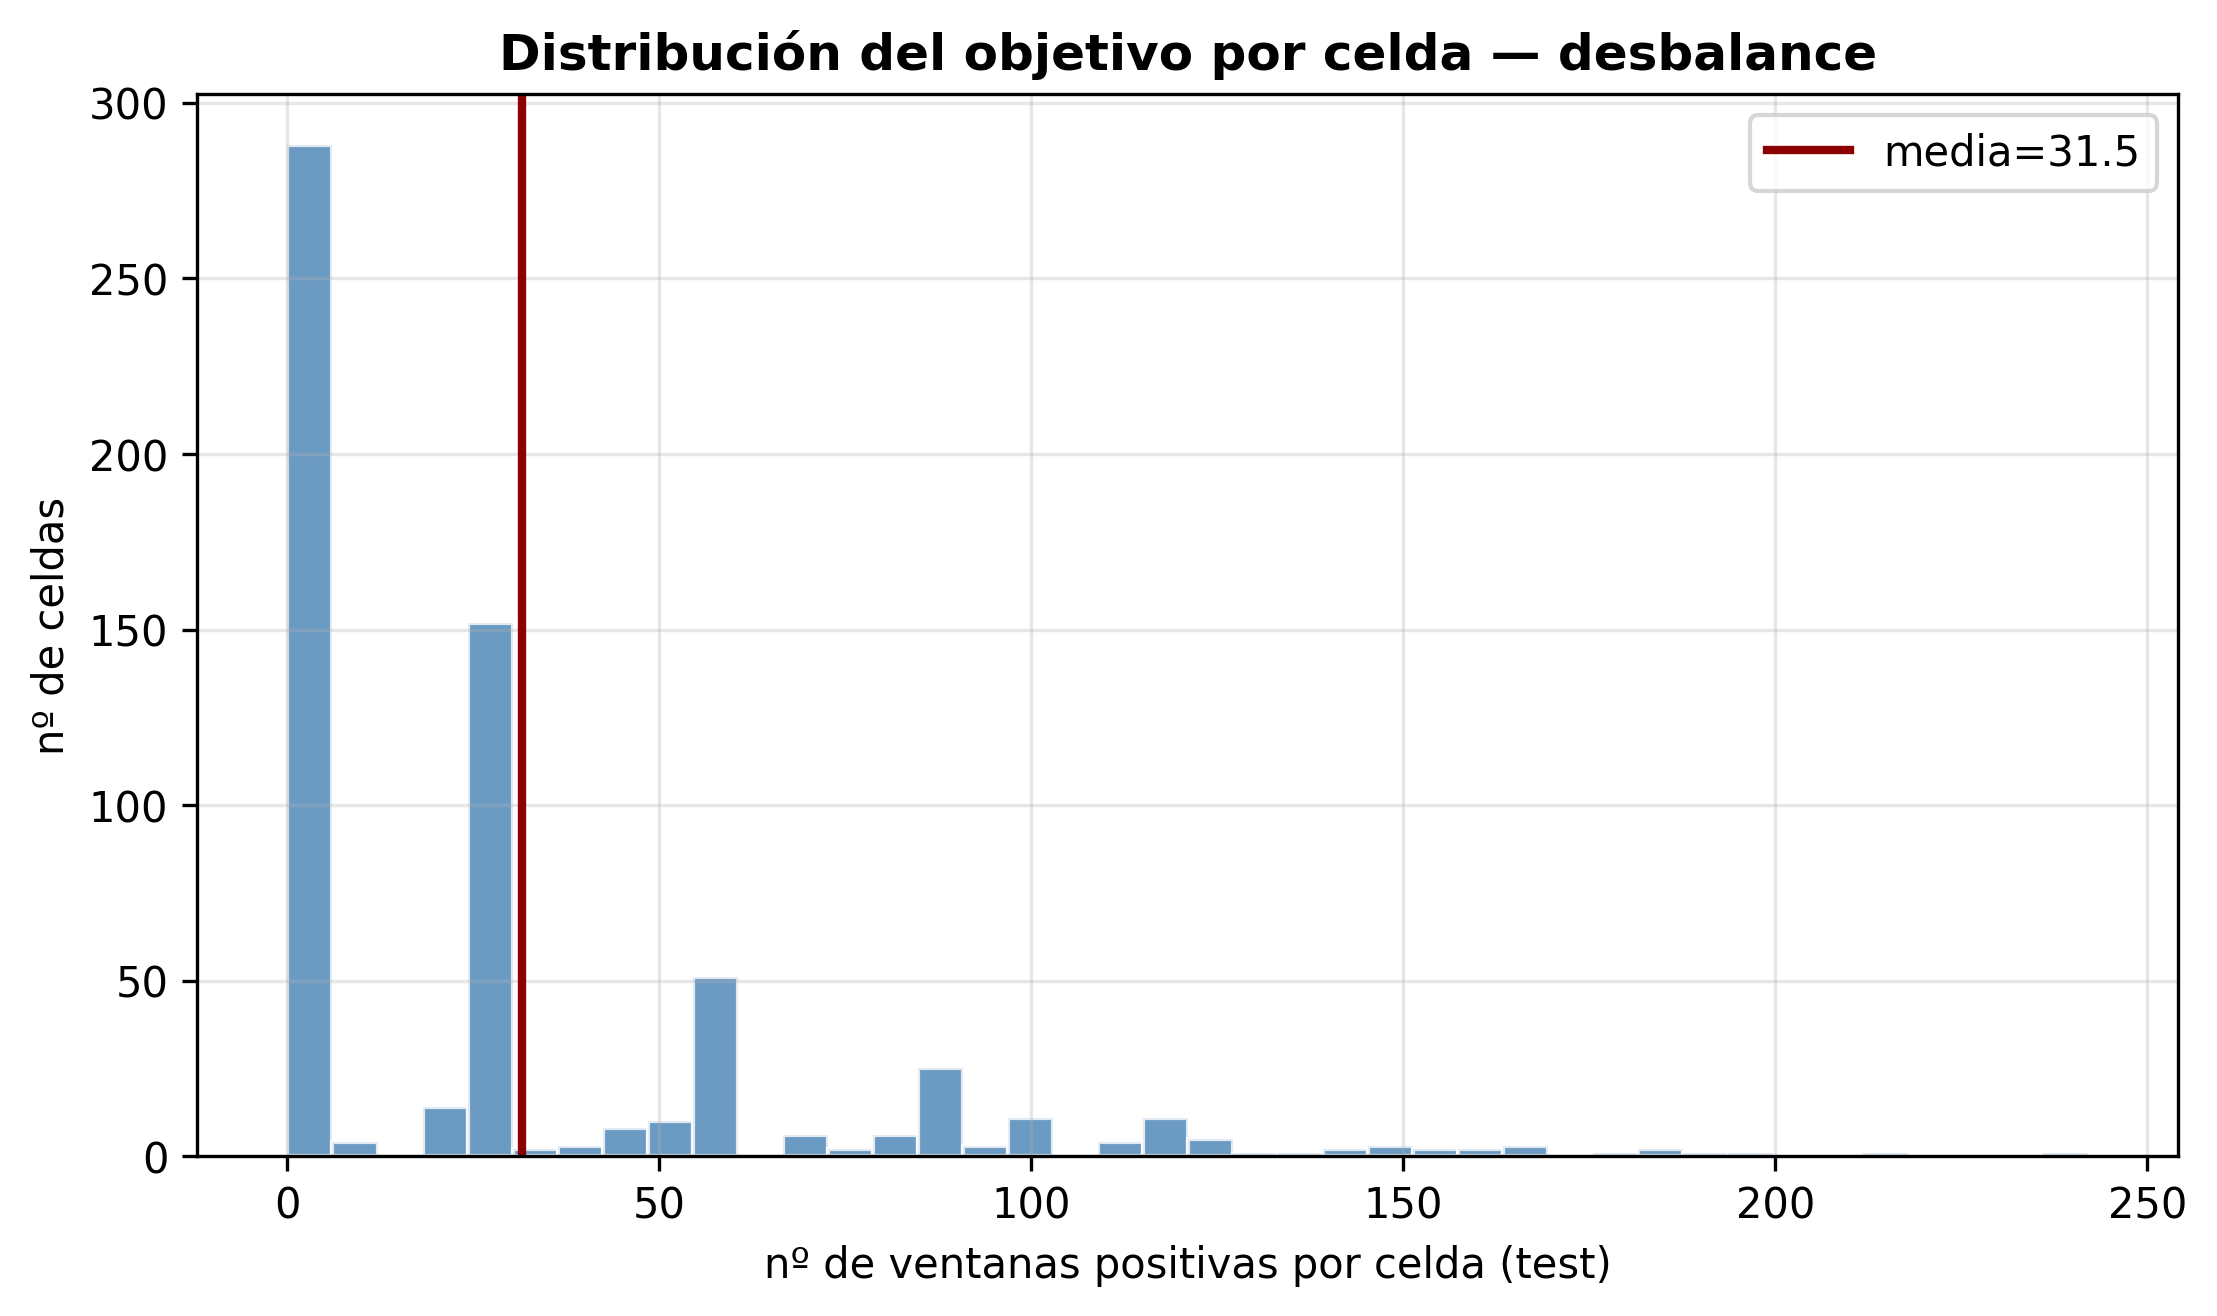
\includegraphics[width=0.78\textwidth]{figuras/04_desbalance}
  \caption[Distribución del objetivo por celda]{\textbf{Distribución del número de ventanas positivas por celda en el conjunto de test.} La mayoría de las celdas registran pocas ventanas con mainshock, mientras que unas pocas concentran la actividad. Este reparto desigual refleja el fuerte desbalance del problema.}
  \label{fig:desbalance}
\end{figure}

El segundo rasgo, más sutil, es que el problema encierra en realidad \textbf{dos preguntas
  distintas}: una espacial (¿qué zonas son peligrosas?) y otra temporal (¿cuándo lo serán?).
Estas dos preguntas tienen una dificultad muy distinta. La primera se apoya en una estructura
estable --las zonas sísmicamente activas lo son de forma persistente-- mientras que la segunda
exige anticipar el momento concreto de un evento, lo que es mucho más difícil. Gran parte del
trabajo de evaluación consiste precisamente en separar ambas, porque mezclarlas en una única
cifra puede dar una impresión equivocada del rendimiento del sistema.

% =============================================================================
\section{Desarrollo del proyecto}
\label{desarrollo-del-proyecto}

Esta sección recorre la construcción de las cinco fases del \textit{pipeline}. Para cada una
se describe qué se implementó y qué decisiones de diseño fueron relevantes; los valores
numéricos se presentan en la Sección~\ref{resultados}.

\subsection{Fase 1: detección y \textit{picking} de fases}
\label{dev-deteccion}

La primera fase valida las herramientas que permiten pasar de una forma de onda a un evento
catalogado. Se emplean dos redes preentrenadas sobre STEAD que representan dos familias
arquitectónicas distintas.

La primera, \textbf{PhaseNet}, es una red convolucional en forma de ``U'' (\textit{U-Net}).
Recibe la traza de tres componentes (las tres direcciones del movimiento del suelo) muestreada
a 100\,Hz y la procesa con una rama descendente de convoluciones y submuestreo, que extrae
características a escalas temporales cada vez más amplias, seguida de una rama ascendente de
sobremuestreo que reconstruye la resolución original. Las conexiones de salto entre ambas ramas
permiten combinar el detalle fino con el contexto global. La salida son tres canales de
probabilidad por cada instante de la traza --onda P, onda S y ruido-- de modo que la llegada de
cada fase se identifica como el máximo del canal correspondiente. Esta arquitectura es
especialmente precisa en la localización temporal, porque conserva la resolución de la señal de
entrada.

La segunda, \textbf{EQTransformer}, es una red más compleja que combina tres ingredientes:
convoluciones para extraer características locales, capas recurrentes bidireccionales que
recorren la traza en ambos sentidos y modelan dependencias de largo alcance, y un mecanismo de
atención que resalta las porciones de la señal relevantes para cada tarea. Su principal ventaja
es que resuelve \emph{tres} tareas a la vez con una sola pasada: detecta si hay un evento en la
traza y, en caso afirmativo, marca las llegadas de las ondas P y S. Esta naturaleza multitarea
la hace muy eficiente para procesar grandes volúmenes de señal continua.

Ambas redes se aplican \emph{sin reentrenar}, sobre un subconjunto de trazas de STEAD no usadas
en su entrenamiento original, y se evalúan comparando las llegadas predichas con las etiquetas
reales bajo varias tolerancias temporales. Esta fase responde a la pregunta de si las
herramientas modernas de detección funcionan de forma fiable sobre datos no vistos, paso previo
imprescindible para cualquier sistema de pronóstico.

El Algoritmo~\ref{alg:deteccion} describe el procedimiento de evaluación de la detección. Como
los modelos están preentrenados, no hay entrenamiento: el algoritmo recorre las trazas, ejecuta
el modelo en inferencia, convierte los canales de probabilidad en llegadas concretas, las
empareja con las llegadas reales dentro de una tolerancia y acumula los aciertos, los fallos y
los errores de tiempo con los que se calculan las métricas finales.

\begin{algorithm}[ht!]
  \caption{Evaluación de la detección y \textit{picking} de fases}
  \label{alg:deteccion}
  \DontPrintSemicolon
  \KwIn{Trazas de STEAD $\{W_i\}$ con llegadas reales de P y S; modelo preentrenado $\mathcal{M}$ (PhaseNet o EQTransformer); tolerancia $\tau$.}
  \KwOut{\textit{Precision}, \textit{recall}, F1 y errores de tiempo (MAE, RMSE) por fase.}
  Inicializar contadores $TP, FP, FN \leftarrow 0$ y lista de errores de tiempo\;
  \For{cada traza $W_i$}{
    $(p^{\text{P}}, p^{\text{S}}, p^{\text{ruido}}) \leftarrow \mathcal{M}(W_i)$ \tcp*{inferencia, sin reentrenar}
    \For{fase $\in \{\text{P}, \text{S}\}$}{
      $t_{\text{pred}} \leftarrow \arg\max_t\, p^{\text{fase}}(t)$ \tcp*{llegada = máximo del canal}
      \eIf{$\exists$ llegada real $t_{\text{real}}$ con $|t_{\text{pred}}-t_{\text{real}}| \leq \tau$}{
        $TP \mathrel{+}= 1$; registrar error $|t_{\text{pred}}-t_{\text{real}}|$\;
      }{
        $FP \mathrel{+}= 1$ (o $FN$ si no hubo predicción para una llegada real)\;
      }
    }
  }
  Calcular \textit{precision}, \textit{recall}, F1~\eqref{eq:f1}, MAE y RMSE\;
  \Return métricas por fase\;
\end{algorithm}

\subsection{Fase 2: red convolucional temporal global}
\label{dev-tcn}

La segunda fase aborda el pronóstico desde la dimensión puramente temporal. La TCN recibe
características agregadas de toda la región --concatenando las de California y las de Alaska--
y predice si habrá un mainshock en los próximos días en \emph{cualquier} punto de la zona. El
objetivo es comprobar si la evolución temporal de la sismicidad, por sí sola, contiene
información suficiente para anticipar eventos. Es, en cierto sentido, el experimento de
control del trabajo: si la señal estuviera en la dimensión temporal global, este modelo
debería capturarla.

Durante el desarrollo se observó un fenómeno relevante al ampliar la ventana de predicción. Al
unir California y Alaska, ambas muy activas, la pregunta ``¿habrá algún mainshock en toda la
región en los próximos 30 días?'' se vuelve casi siempre afirmativa, porque en una región tan
grande y activa suele ocurrir algún evento moderado en cualquier ventana de un mes. Esto
convierte el objetivo en degenerado y poco informativo, y motivó mantener la formulación global
con una ventana más corta. Este comportamiento ilustra por qué una formulación \emph{espacial},
que pregunta por celdas concretas en lugar de por toda la región, es más adecuada: en ella el
objetivo sí discrimina.

\subsection{Fase 3: red neuronal de grafos espacial}
\label{dev-gnn}

La tercera fase introduce la dimensión espacial. El modelo procesa la serie temporal de cada
celda con una TCN compartida y a continuación propaga información entre celdas vecinas mediante
dos capas de grafo, de modo que la predicción de una celda incorpora no solo su propia
historia, sino también la de su entorno. Esta fase pone a prueba la hipótesis de que la señal
aprovechable reside en los patrones espaciales locales y no en agregaciones globales. La
construcción del grafo, descrita en la Sección~\ref{md-grafo}, respeta la separación entre las
dos regiones.

En la implementación, el procesamiento se realiza por lotes de días completos: cada ejemplo de
entrenamiento es una ``foto'' de toda la región en un instante, con sus celdas y su grafo, lo
que permite que la propagación espacial actúe sobre el estado simultáneo de todas las celdas.
La matriz de adyacencia normalizada se precalcula una sola vez, ya que el grafo es fijo, lo que
hace muy eficiente cada paso de propagación. El número de parámetros se mantiene en el orden de
las decenas de miles gracias a que la TCN comparte pesos entre todas las celdas; esta economía
de parámetros es deliberada y especialmente importante en un problema con relativamente pocos
ejemplos positivos, porque reduce el riesgo de sobreajuste. Durante el desarrollo se comprobó
que la profundidad de dos capas de grafo ofrece el mejor equilibrio: con una sola capa la
información apenas se propaga, y con más de dos aparece el fenómeno de sobre-suavizado, por el
que las celdas tienden a parecerse entre sí y se pierde la discriminación local.

\subsection{Fase 4: Transformer geoespacial}
\label{dev-transformer}

La cuarta fase explora una segunda forma de modelar el espacio. En lugar de imponer un grafo de
vecindad fijo, el Transformer deja que el mecanismo de atención aprenda qué celdas son
relevantes para cada predicción, usando la codificación de las coordenadas geográficas. Comparte
el mismo procesamiento temporal que la GNN, de modo que la comparación entre ambos aísla el
efecto del mecanismo de mezcla espacial. Durante el desarrollo se introdujeron dos mejoras que
resultaron beneficiosas: el uso del \textit{pooling} temporal completo (estado final, media y
máximo) a la entrada del bloque de atención, y la máscara que restringe la atención al interior
de cada región. Con ellas, el Transformer se convirtió en el modelo espacial con mejor
rendimiento del trabajo.

La diferencia conceptual con la GNN merece subrayarse. La red de grafos parte de una hipótesis
fuerte --que las celdas relevantes son las geográficamente próximas-- y la codifica en un grafo
fijo. El Transformer, en cambio, no impone esa hipótesis: deja que los datos decidan, para cada
celda, a cuáles otras conviene atender, ponderando su contribución mediante pesos aprendidos. La
codificación posicional sinusoidal de las coordenadas le proporciona el sentido de la geografía
que el grafo le daba de forma explícita a la GNN, pero de manera más flexible. La máscara por
regiones actúa como una restricción mínima e indiscutible --no tiene sentido que una celda de
California atienda a una de Alaska-- que reduce el espacio de búsqueda y estabiliza el
entrenamiento sin imponer una estructura de vecindad rígida. El hecho de que esta mayor
flexibilidad se traduzca en un rendimiento ligeramente superior sugiere que la noción de
``vecindad relevante'' en sismicidad es algo más rica que la simple proximidad geográfica.

\subsection{Fase 5: Proceso Gaussiano y mapas de riesgo}
\label{dev-gp}

La quinta fase cierra el \textit{pipeline} transformando las predicciones discretas por celda
en un producto cartográfico. El proceso gaussiano interpola las probabilidades sobre una
rejilla fina, produciendo una superficie continua de riesgo, y aporta además una estimación de
incertidumbre en cada punto. El procedimiento consta de tres pasos encadenados. Primero, se
toman las probabilidades del Transformer en los centroides de las celdas activas y se promedian
sobre el periodo de evaluación para obtener un valor de riesgo representativo por celda.
Segundo, esas probabilidades se \emph{calibran} mediante regresión isotónica, una técnica que
ajusta una función monótona para que las probabilidades predichas coincidan con las frecuencias
observadas; este paso es necesario porque la ponderación de clase usada en el entrenamiento
infla las probabilidades crudas, y la calibración se ajusta sobre una mitad del test y se valida
sobre la otra para evitar circularidad. Tercero, el proceso gaussiano interpola esos valores
calibrados sobre una rejilla fina, ajustando los parámetros de su \textit{kernel} de Matérn por
máxima verosimilitud de forma independiente en cada región. El resultado son dos mapas por
región: uno de riesgo y otro de
incertidumbre.

El Algoritmo~\ref{alg:gp} recoge estos tres pasos --promediado, calibración e interpolación--
y muestra cómo el proceso gaussiano entrega a la vez el mapa de riesgo (su media) y el de
incertidumbre (su desviación) en cada punto de la rejilla.

\begin{algorithm}[ht!]
  \caption{Cartografía del riesgo con calibración y Proceso Gaussiano}
  \label{alg:gp}
  \DontPrintSemicolon
  \KwIn{Probabilidades del Transformer por celda y día; centroides de las celdas activas; rejilla fina de salida.}
  \KwOut{Mapa de riesgo y mapa de incertidumbre por región.}
  $\bar{p}_c \leftarrow$ media temporal de la probabilidad en cada celda $c$ \tcp*{un valor por celda}
  Ajustar la regresión isotónica $g(\cdot)$ en una mitad del test; validar en la otra\;
  $r_c \leftarrow g(\bar{p}_c)$ \tcp*{probabilidades calibradas}
  \For{cada región (California, Alaska)}{
    Ajustar el GP (\textit{kernel} Matérn) por máxima verosimilitud sobre $\{(\text{centroide}_c, r_c)\}$\;
    \For{cada punto $\mathbf{x}_*$ de la rejilla}{
      $\mu_* \leftarrow \mathbf{k}_*^\top (K+\sigma^2 I)^{-1} \mathbf{r}$ \tcp*{riesgo interpolado}
      $\sigma_*^2 \leftarrow k(\mathbf{x}_*,\mathbf{x}_*) - \mathbf{k}_*^\top (K+\sigma^2 I)^{-1}\mathbf{k}_*$ \tcp*{incertidumbre}
    }
  }
  \Return mapa de riesgo $\mu$ y mapa de incertidumbre $\sigma$\;
\end{algorithm}

% =============================================================================
\section{Resultados}
\label{resultados}

Esta sección presenta los resultados de las cinco fases. Se comienza por la detección, se
continúa con la comparación de los modelos de pronóstico y su análisis espacial y temporal, se
añaden las métricas operativas y los estudios de ablación, y se cierra con los mapas de riesgo
y la discusión de los resultados en el contexto del estado del arte.

\subsection{Detección y \textit{picking} de fases}
\label{res-deteccion}

La Tabla~\ref{tab:deteccion} recoge el rendimiento de PhaseNet y EQTransformer en la
identificación de las llegadas de las ondas P y S, con una tolerancia de 0.1\,s. Ambas redes
alcanzan un rendimiento alto, especialmente en la onda P, que es la más nítida. PhaseNet obtiene
un \textit{F1-score}~\eqref{eq:f1} de 0.93 en la fase P y de 0.79 en la fase S, con errores
medios de localización de pocas centésimas de segundo, comparables a los de un analista humano.
EQTransformer ofrece un rendimiento ligeramente inferior en este subconjunto pero igualmente
sólido, con la ventaja de resolver las tres tareas (detección, P y S) en una sola pasada.

\begin{table}[ht!]
  \centering
  \small
  \begin{tabular}{@{}llccccc@{}}
    \toprule
    \textbf{Modelo} & \textbf{Fase} & \textbf{Precision} & \textbf{Recall} & \textbf{F1}    & \textbf{MAE (s)} & \textbf{RMSE (s)} \\
    \midrule
    PhaseNet        & P             & 0.927              & 0.934           & \textbf{0.930} & 0.022            & 0.030             \\
    PhaseNet        & S             & 0.782              & 0.794           & 0.788          & 0.029            & 0.038             \\
    EQTransformer   & P             & 0.883              & 0.787           & 0.832          & 0.027            & 0.036             \\
    EQTransformer   & S             & 0.739              & 0.760           & 0.750          & 0.035            & 0.044             \\
    \bottomrule
  \end{tabular}
  \caption[Resultados de detección y \textit{picking} de fases P y S]{\textbf{Rendimiento en detección y \textit{picking}} de PhaseNet y EQTransformer sobre STEAD (tolerancia 0.1\,s). MAE y RMSE son los errores de localización temporal de la llegada, en segundos.}
  \label{tab:deteccion}
\end{table}

Estos resultados confirman que las herramientas de detección basadas en aprendizaje profundo funcionan
de forma fiable sobre datos no vistos y constituyen una base firme sobre la que apoyar el resto
del sistema.

\begin{figure}[ht!]
  \centering
  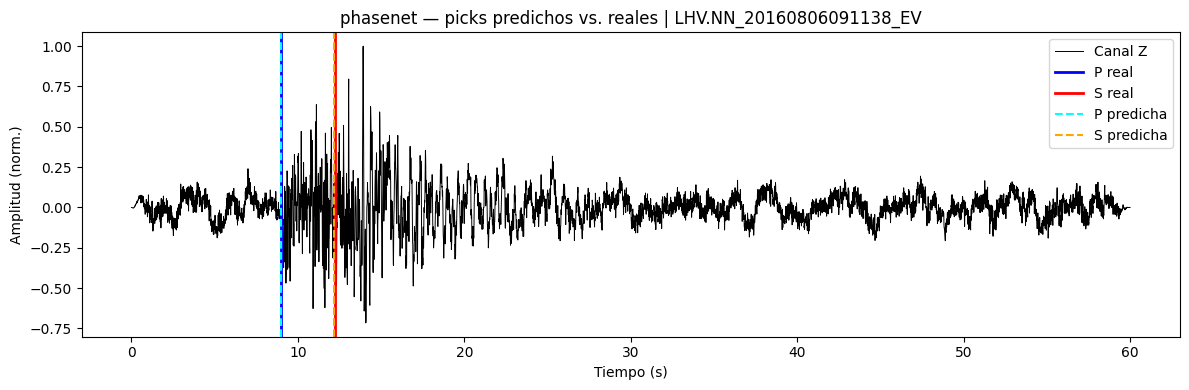
\includegraphics[width=0.92\textwidth]{figuras/output_phasnet}
  \caption[Ejemplo de detección y \textit{picking} con PhaseNet]{\textbf{Ejemplo de detección y \textit{picking} con PhaseNet} sobre una traza de STEAD. Se muestran las componentes de la forma de onda junto con las probabilidades de fase predichas por la red y las llegadas estimadas de las ondas P y S.}
  \label{fig:output-phasenet}
\end{figure}

\begin{figure}[ht!]
  \centering
  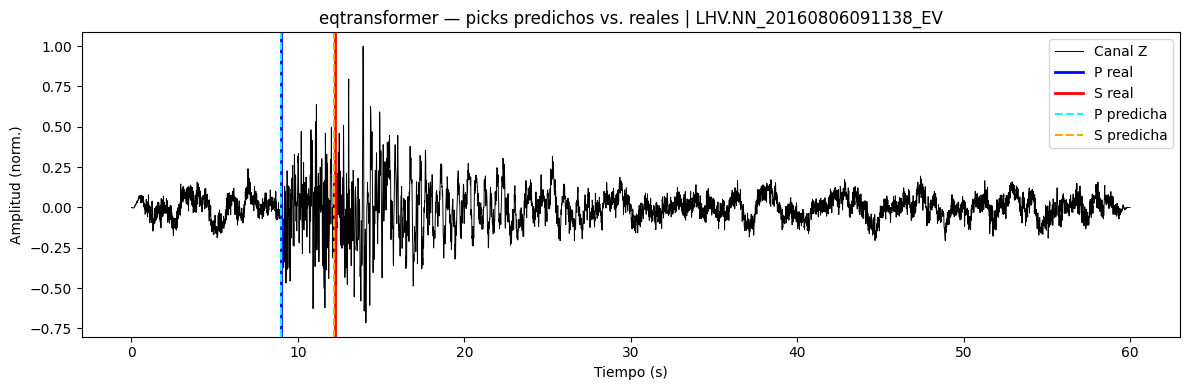
\includegraphics[width=0.92\textwidth]{figuras/output_eqtransformer}
  \caption[Ejemplo de detección y \textit{picking} con EQTransformer]{\textbf{Ejemplo de detección y \textit{picking} con EQTransformer} sobre una traza de STEAD. Junto a la forma de onda se representan las probabilidades de detección del evento y de las llegadas de las ondas P y S obtenidas en una sola pasada.}
  \label{fig:output-eqtransformer}
\end{figure}

La tolerancia de 0.1\,s es exigente: equivale a acertar la llegada con un margen de diez
muestras a 100\,Hz. Conviene comprobar cómo evoluciona el rendimiento al relajar este margen,
porque en muchas aplicaciones operativas un error de unas décimas de segundo es perfectamente
asumible. La Tabla~\ref{tab:deteccion-umbral} recoge el \textit{F1-score} de la fase P de
PhaseNet para tres tolerancias. Como cabe esperar, el rendimiento crece al ampliar la
tolerancia: con un margen de medio segundo el \textit{F1} supera el 0.96, lo que confirma que
la inmensa mayoría de las llegadas se detectan correctamente y que los pocos fallos a tolerancia
estricta corresponden a pequeñas desviaciones en la localización, no a detecciones perdidas.

\begin{table}[ht!]
  \centering
  \small
  \begin{tabular}{@{}lccc@{}}
    \toprule
    \textbf{Tolerancia} & \textbf{0.1\,s} & \textbf{0.3\,s} & \textbf{0.5\,s} \\
    \midrule
    \textit{F1} fase P  & 0.930           & 0.951           & 0.963           \\
    \bottomrule
  \end{tabular}
  \caption[Sensibilidad de la detección a la tolerancia temporal]{\textbf{\textit{F1-score} de la fase P (PhaseNet) según la tolerancia temporal.} Al relajar el margen de acierto, el rendimiento aumenta, lo que indica que los errores se concentran en pequeñas desviaciones de localización y no en detecciones omitidas.}
  \label{tab:deteccion-umbral}
\end{table}

\subsection{Comparación de los modelos de pronóstico}
\label{res-comparativa}

La Tabla~\ref{tab:comparativa} reúne el rendimiento de todos los modelos de pronóstico sobre el
conjunto de test (2023--2024), junto con las tres referencias. Todos los modelos espaciales se
evalúan sobre el mismo objetivo, de modo que las cifras son directamente comparables. Para los
modelos con varias semillas se indica la media y la desviación típica.

\begin{table}[ht!]
  \centering
  \small
  \begin{tabular}{@{}lcc@{}}
    \toprule
    \textbf{Modelo}               & \textbf{AUC-ROC (test)}    & \textbf{Tipo}       \\
    \midrule
    Persistencia                  & 0.513                      & referencia temporal \\
    Regresión logística           & 0.544                      & referencia lineal   \\
    TCN global (Fase 2)           & 0.512 $\pm$ 0.052          & temporal            \\
    \midrule
    Poisson (climatología)        & 0.726                      & referencia espacial \\
    GNN (Fase 3)                  & 0.699 $\pm$ 0.008          & espacial            \\
    \textbf{Transformer (Fase 4)} & \textbf{0.728 $\pm$ 0.002} & espacial            \\
    \bottomrule
  \end{tabular}
  \caption[Comparativa de los modelos de pronóstico frente a las referencias]{\textbf{Resultados de pronóstico en test (2023--2024).} AUC-ROC de cada modelo frente a las referencias. La persistencia, la regresión logística y el TCN operan sobre objetivos globales o lineales; los modelos espaciales y el Poisson comparten el objetivo por celda. Para los modelos entrenados con varias semillas, el valor es la media y el \(\pm\) la \textbf{desviación típica muestral} (dividiendo entre \(N-1\)) del AUC sobre las cinco semillas \{13, 42, 123, 256, 1024\}.}
  \label{tab:comparativa}
\end{table}

Los resultados permiten una lectura clara. En el bloque temporal, ni la persistencia, ni la
regresión logística, ni el TCN superan de forma apreciable el nivel del azar: el TCN global
alcanza un AUC de 0.512 y un test estadístico confirma que no mejora a la regresión logística
de manera significativa. Esto indica que la dimensión temporal global, por sí sola, no contiene
información suficiente para el pronóstico, y justifica el paso a una formulación espacial. La
Figura~\ref{fig:roctcn} lo ilustra: las curvas ROC del TCN se mantienen muy próximas a la
diagonal del azar.

\begin{figure}[ht!]
  \centering
  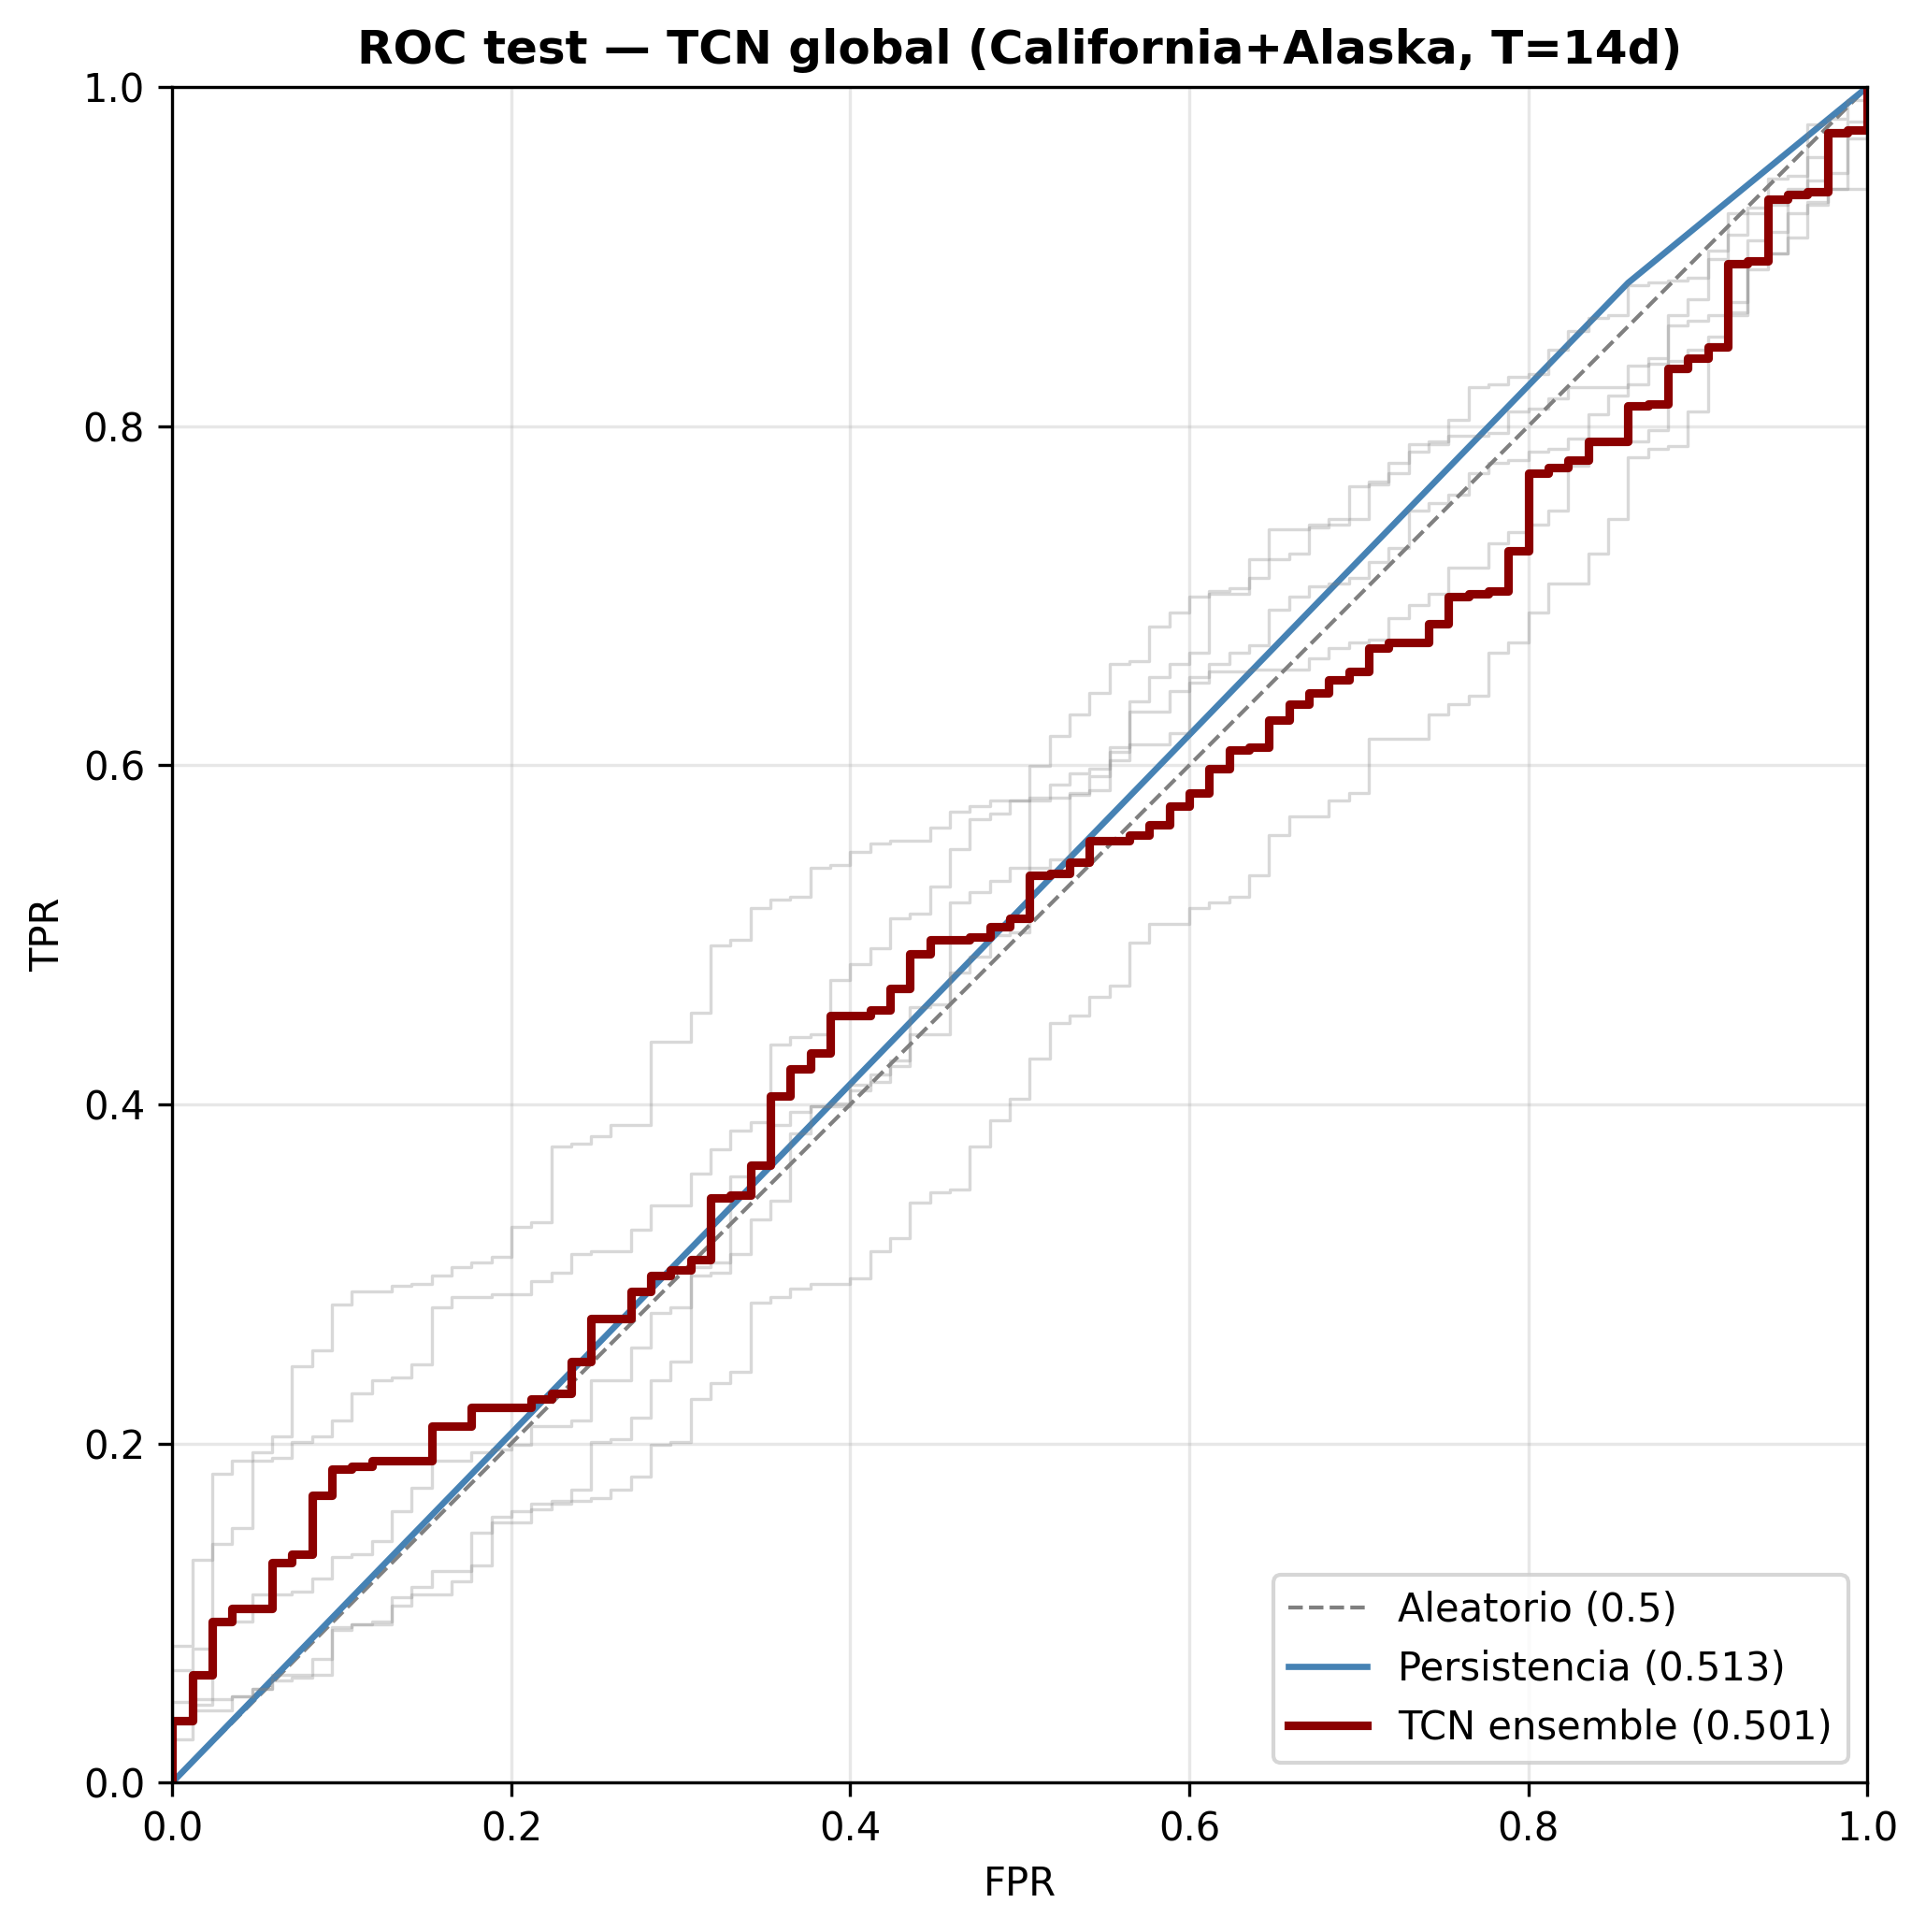
\includegraphics[width=0.64\textwidth]{figuras/03_roc_test}
  \caption[Curva ROC del TCN temporal global]{\textbf{Curvas ROC en test del TCN temporal global.} En gris, las cinco semillas; en rojo, el \textit{ensemble}; en azul, la persistencia. La proximidad a la diagonal indica que el enfoque temporal global no aporta capacidad discriminativa.}
  \label{fig:roctcn}
\end{figure}

En el bloque espacial el panorama cambia. Tanto la GNN como el Transformer alcanzan un AUC en
torno a 0.70--0.73, muy por encima de las referencias temporales. El \textbf{Transformer es
  el mejor modelo}, con un AUC de \(0.728 \pm 0.002\) que supera a la climatología de Poisson de
forma estadísticamente significativa: un \emph{t}-test de una muestra de las cinco semillas
frente a la tasa base del Poisson da \(t = 2.6\) y \(p = 0.029\) (contraste unilateral). La GNN,
con \(0.699\), queda ligeramente por debajo del Poisson. La superioridad del Transformer sobre la
GNN también se confirma con un test no paramétrico: un \textbf{Wilcoxon pareado} sobre las cinco
semillas comunes --donde el Transformer gana a la GNN en las cinco-- arroja \(p = 0.031\)
(unilateral); el equivalente \emph{t}-test pareado, más potente con tan pocas muestras, da
\(p = 0.001\). La estabilidad de estos resultados se aprecia en la
Tabla~\ref{tab:perseed}, que detalla el AUC de cada semilla: la desviación típica es muy pequeña,
del orden de la milésima en el Transformer, lo que indica que los valores no dependen del azar de
una ejecución concreta sino que son una propiedad robusta del modelo y de los datos. De hecho, el
\textbf{intervalo de confianza al 95\,\%} del AUC, estimado con la distribución \emph{t} de
Student sobre las cinco semillas, es estrecho y no incluye al azar: \([0.725,\,0.731]\) para el
Transformer y \([0.690,\,0.709]\) para la GNN. La Figura~\ref{fig:curvas} muestra las curvas de
entrenamiento del Transformer, con una convergencia muy consistente entre semillas.

\begin{table}[ht!]
  \centering
  \small
  \begin{tabular}{@{}lccccccc@{}}
    \toprule
    \textbf{Modelo} & \textbf{s.\,13} & \textbf{s.\,42} & \textbf{s.\,123} & \textbf{s.\,256} & \textbf{s.\,1024} & \textbf{media\(\pm\)std} & \textbf{ens.} \\
    \midrule
    GNN             & 0.694           & 0.703           & 0.711            & 0.694            & 0.694             & 0.699\(\pm\)0.008        & 0.702         \\
    Transformer     & 0.732           & 0.728           & 0.728            & 0.726            & 0.726             & 0.728\(\pm\)0.002        & 0.729         \\
    \bottomrule
  \end{tabular}
  \caption[AUC de test por semilla de los modelos espaciales]{\textbf{AUC-ROC en test para cada semilla.} La baja dispersión entre semillas confirma que los resultados son estables y reproducibles. La columna media\(\pm\)std recoge la media y la \textbf{desviación típica muestral} (\(N-1\)) sobre las cinco semillas; el \textit{ensemble} promedia las cinco predicciones.}
  \label{tab:perseed}
\end{table}

\begin{figure}[ht!]
  \centering
  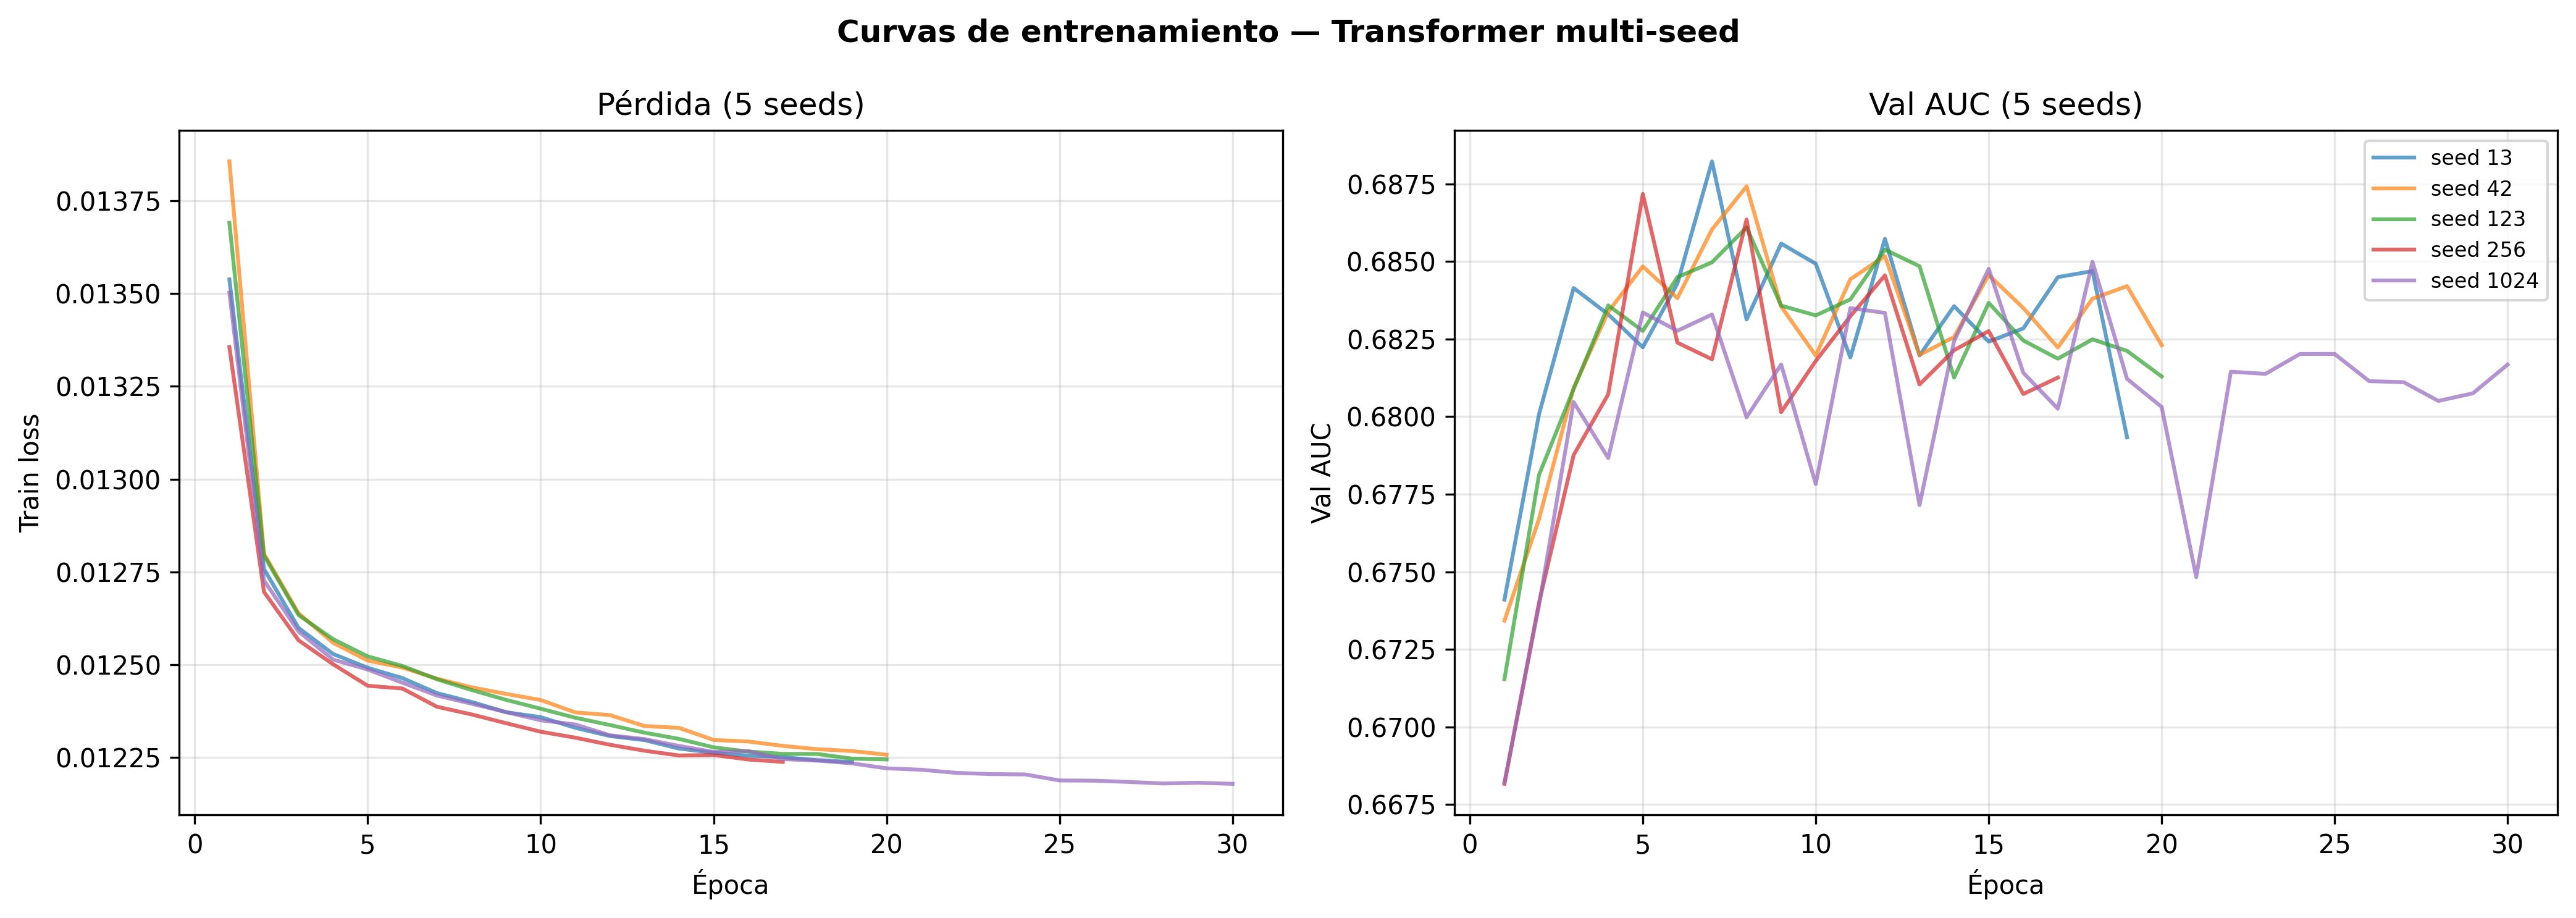
\includegraphics[width=\textwidth]{figuras/05_curvas_multiseed}
  \caption[Curvas de entrenamiento del Transformer multi-semilla]{\textbf{Curvas de entrenamiento del Transformer} para las cinco semillas. Izquierda: pérdida de entrenamiento. Derecha: AUC de validación por época. La convergencia consistente entre semillas refleja un entrenamiento estable.}
  \label{fig:curvas}
\end{figure}

Para visualizar de un vistazo cómo se sitúan los tres modelos espaciales, la
Figura~\ref{fig:comparativa} compara sus métricas en dos paneles. El panel de la izquierda
muestra la capacidad discriminativa (AUC-ROC y PR-AUC) y el de la derecha el rendimiento
operativo (\textit{lift} en los dos niveles de alarma). La lectura conjunta es clara: el
Transformer y el Poisson van prácticamente a la par y por delante de la GNN en todas las
métricas. La diferencia es especialmente visible en el \textit{lift} y en la PR-AUC, donde la
GNN se queda algo por detrás de la climatología, mientras que el Transformer la iguala o la
supera ligeramente. Esta figura resume el mensaje central de la comparación: el Transformer es
el modelo de aprendizaje profundo que logra ponerse al nivel de la mejor referencia y rebasarla.

\begin{figure}[ht!]
  \centering
  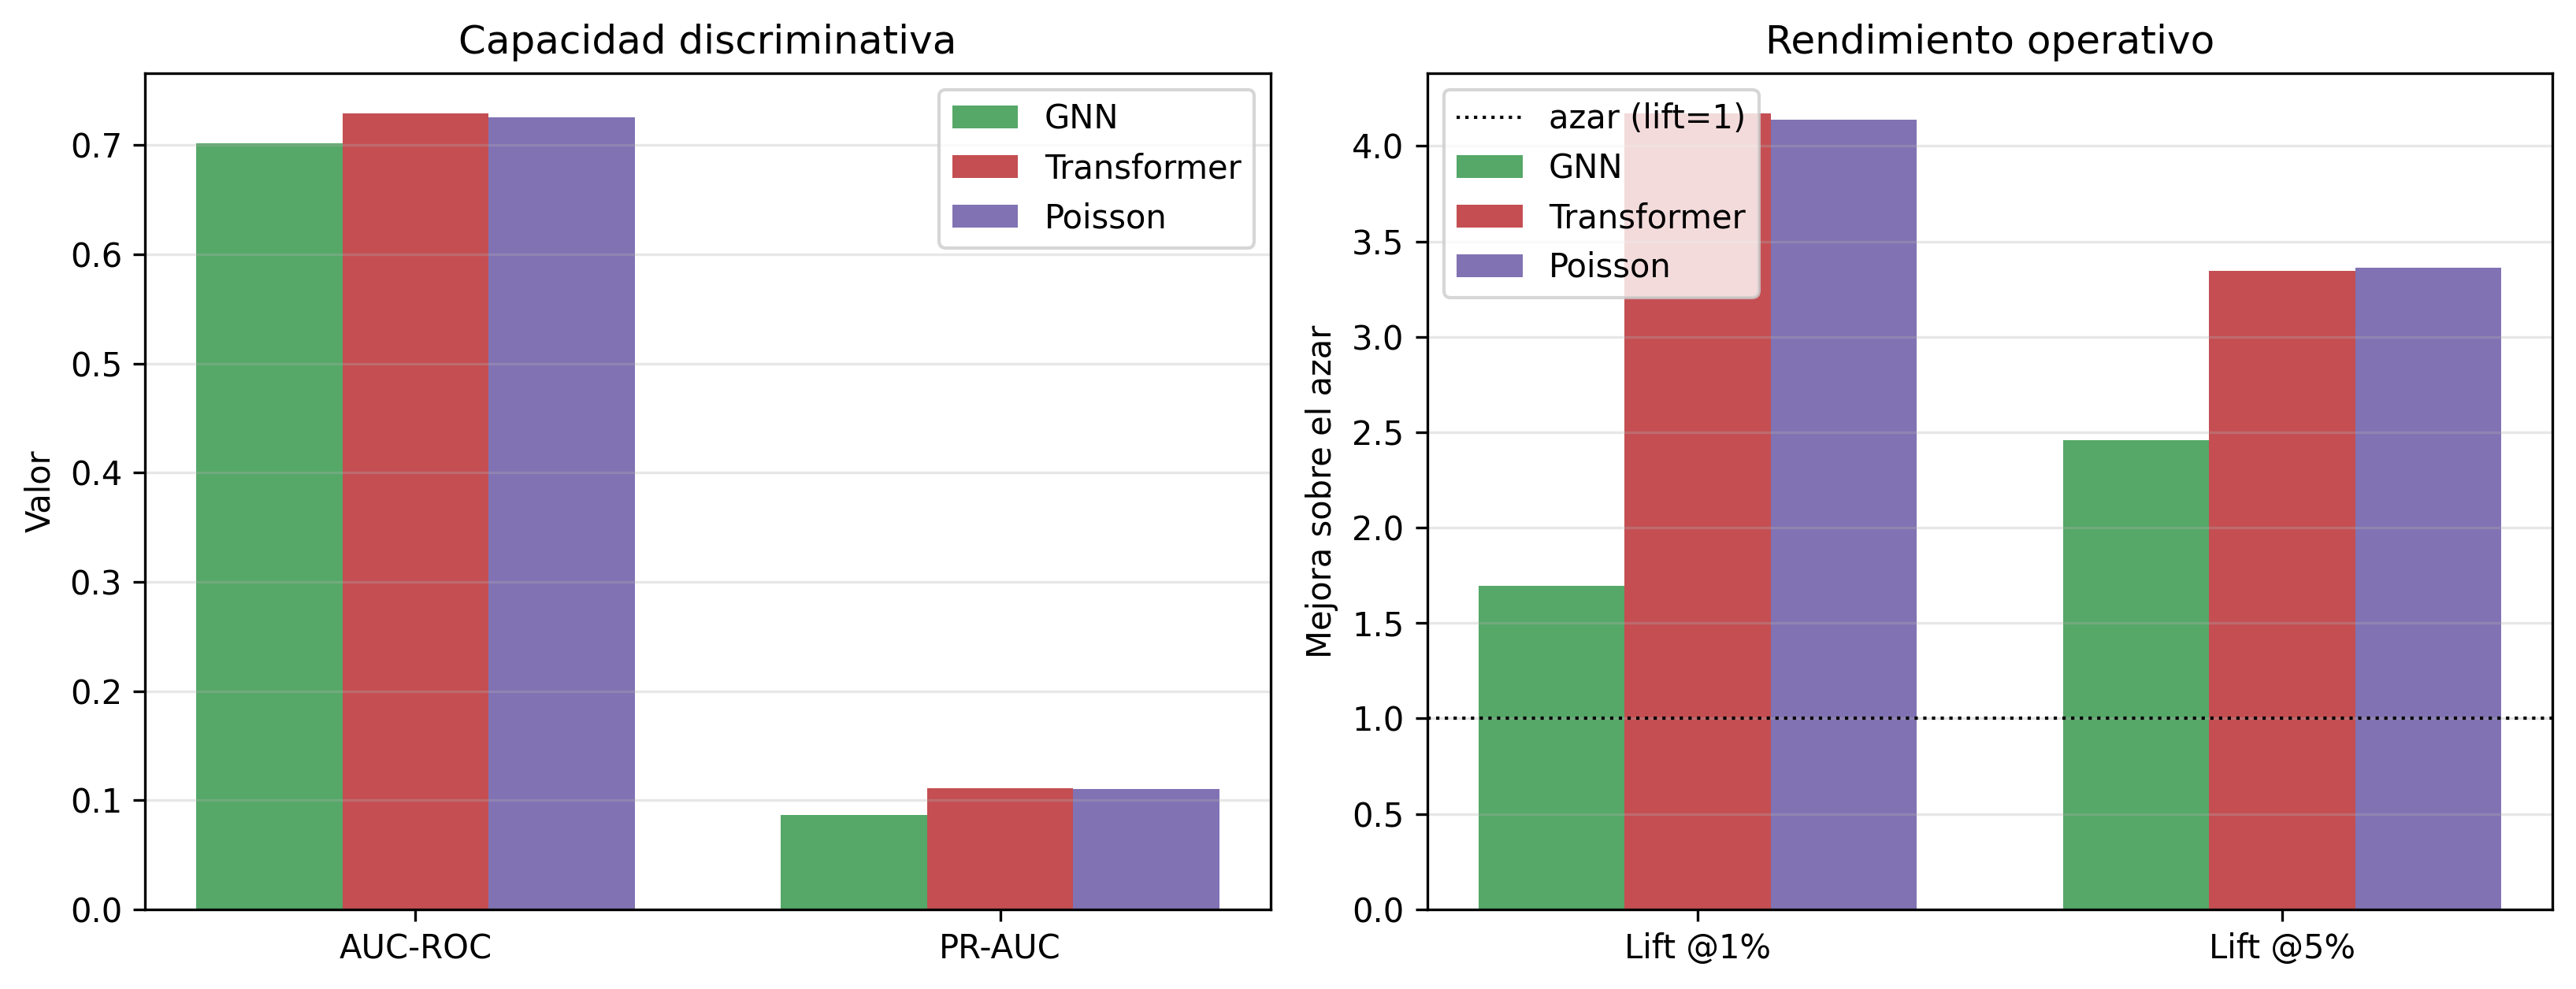
\includegraphics[width=\textwidth]{figuras/comparativa_modelos}
  \caption[Comparativa de métricas entre modelos espaciales]{\textbf{Comparativa de métricas de los modelos espaciales frente al Poisson.} Izquierda: capacidad discriminativa (AUC-ROC y PR-AUC). Derecha: rendimiento operativo (\textit{lift} en el top 1\,\% y 5\,\%; la línea de puntos marca el azar). El Transformer iguala o supera a la climatología en todas las métricas, mientras que la GNN queda algo por detrás.}
  \label{fig:comparativa}
\end{figure}

\subsection{Curvas ROC y diagrama de Molchan}
\label{res-roc-molchan}

La Figura~\ref{fig:roc} muestra las curvas ROC del Transformer y del Poisson sobre el test. Ambas
quedan claramente por encima de la diagonal del azar, lo que refleja una capacidad de
discriminación apreciable. La Figura~\ref{fig:molchan} presenta el mismo resultado en el formato
del diagrama de Molchan, habitual en sismología: la curva del Transformer cae por debajo de la
diagonal, señal de un \textit{skill} positivo, y muy próxima a la del Poisson.

\begin{figure}[ht!]
  \centering
  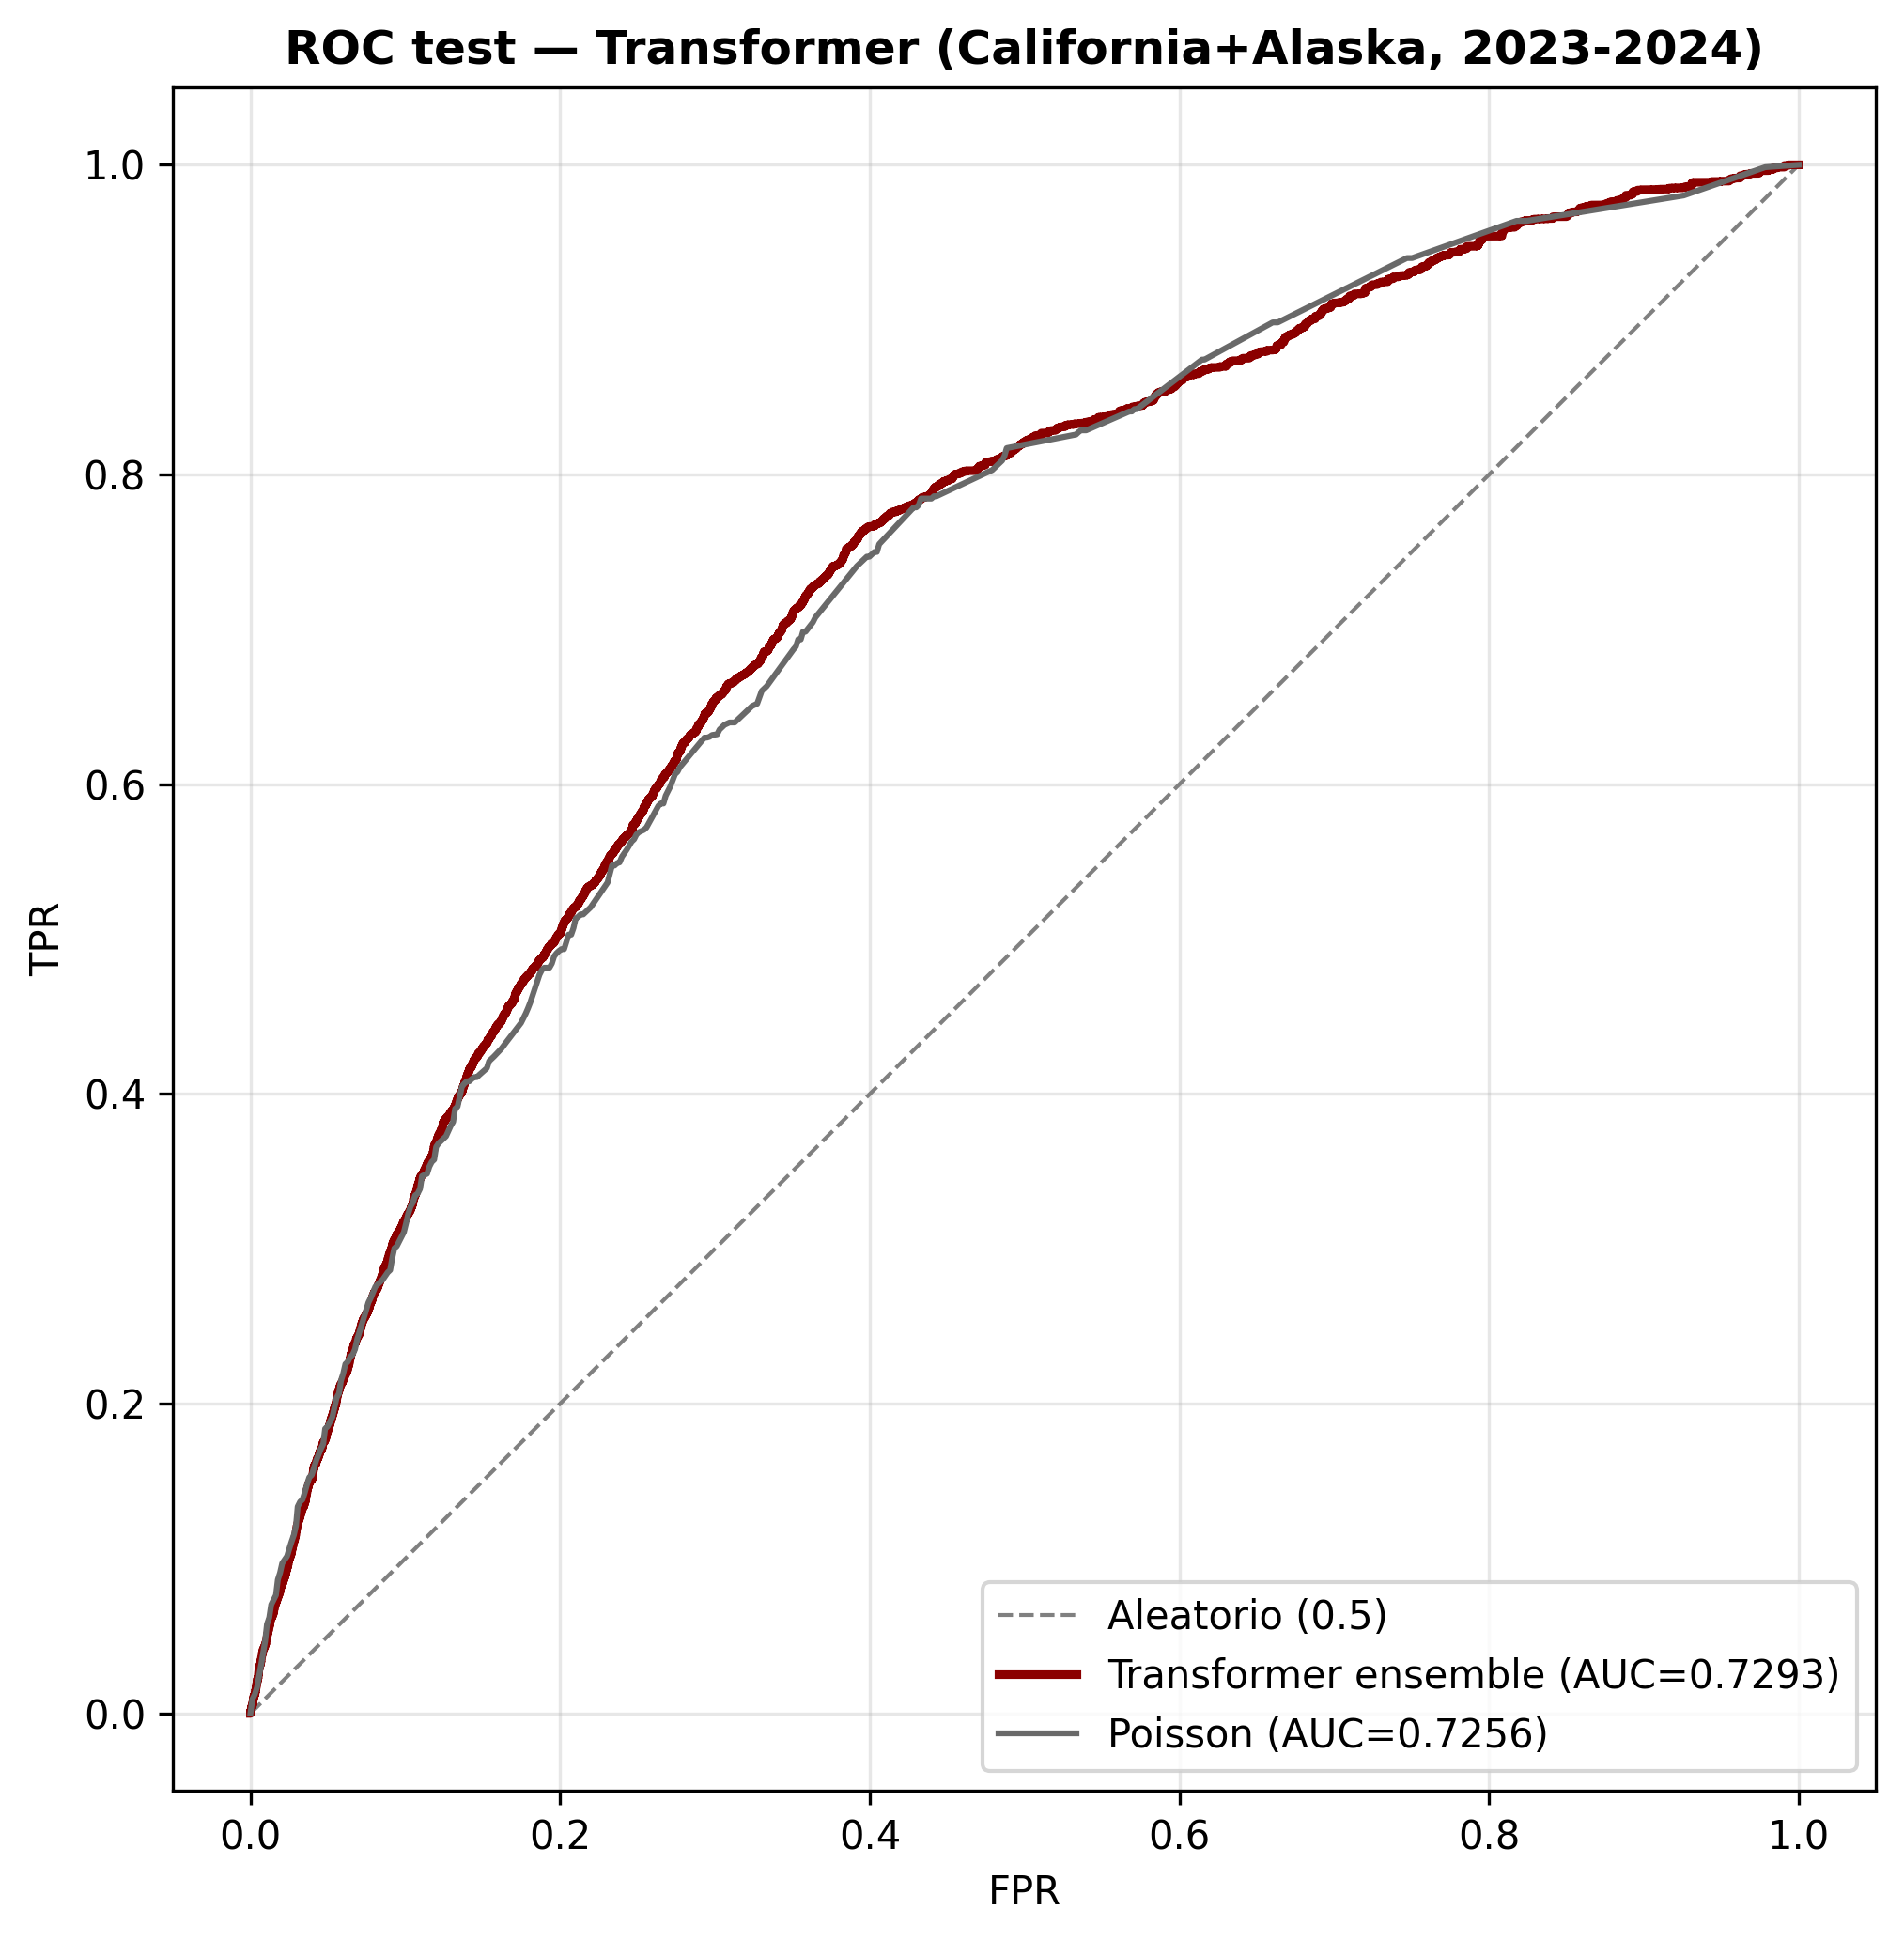
\includegraphics[width=0.66\textwidth]{figuras/05_roc_test}
  \caption[Curva ROC del Transformer en test]{\textbf{Curva ROC en test (2023--2024)} del \textit{ensemble} del Transformer geoespacial frente al modelo de Poisson. Ambos superan claramente la diagonal del azar.}
  \label{fig:roc}
\end{figure}

\begin{figure}[ht!]
  \centering
  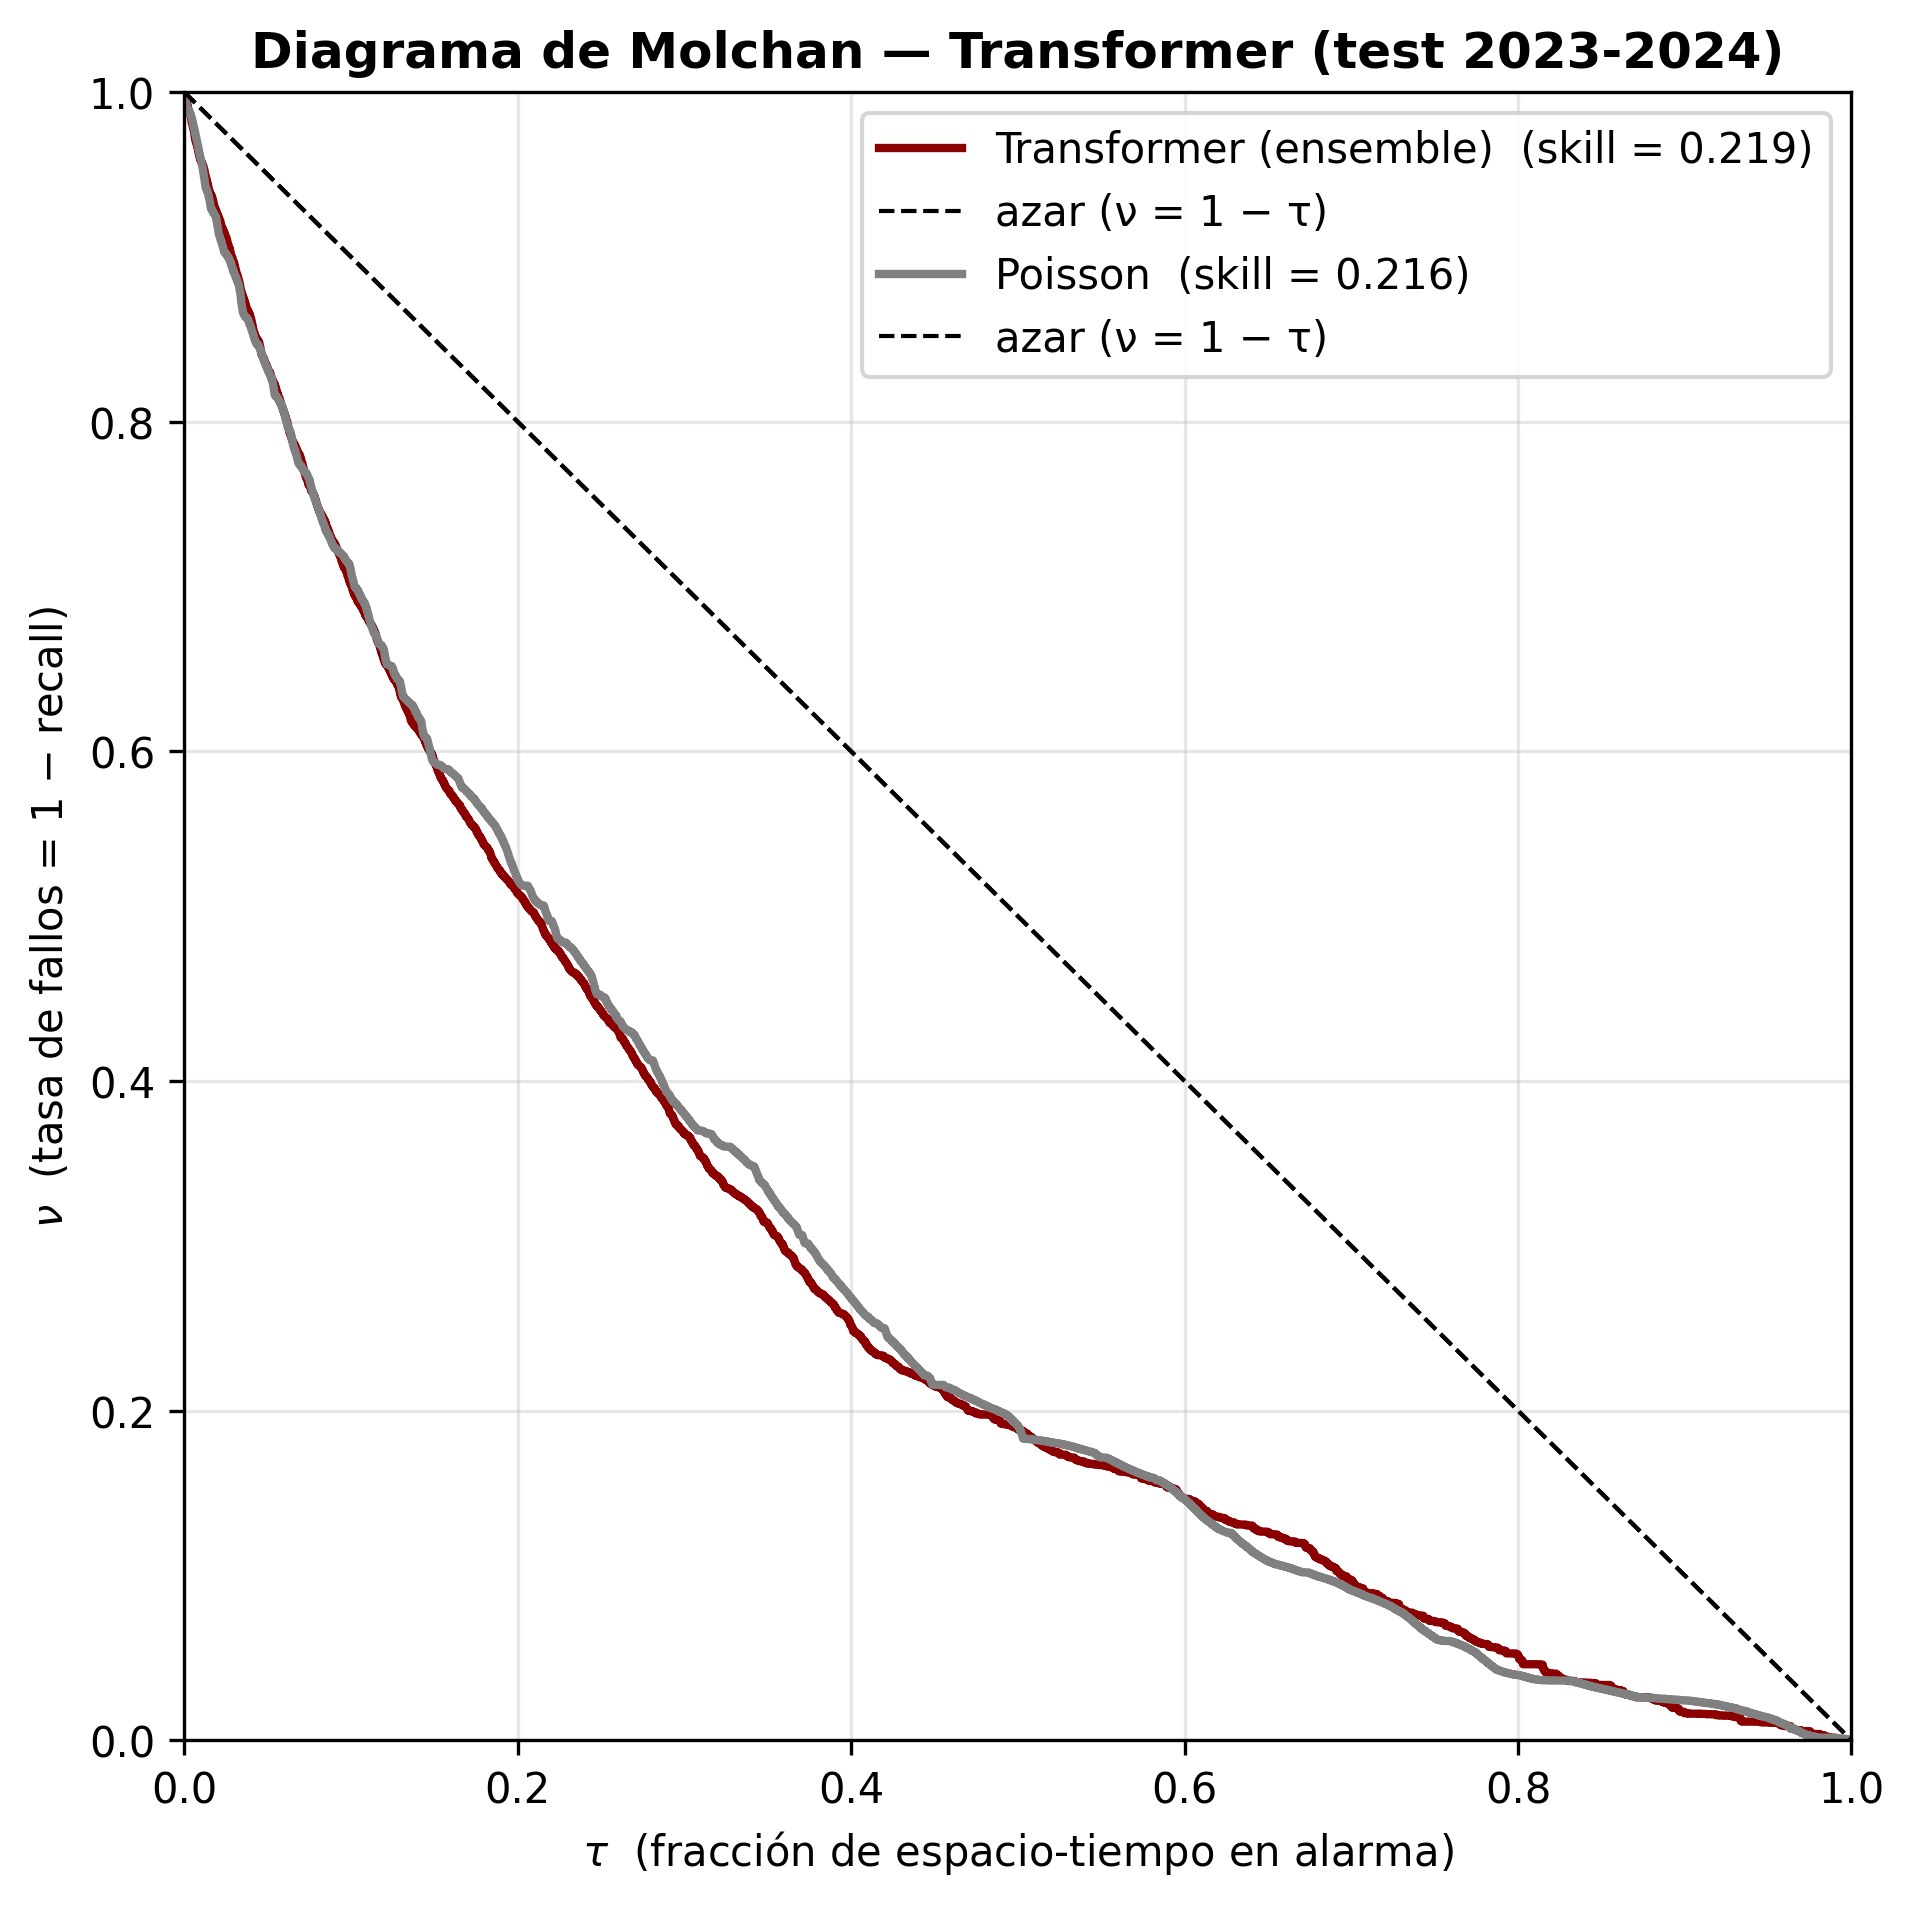
\includegraphics[width=0.62\textwidth]{figuras/05_molchan}
  \caption[Diagrama de Molchan del Transformer]{\textbf{Diagrama de Molchan} del Transformer frente al Poisson. La curva por debajo de la diagonal indica habilidad predictiva; el área entre la curva y la diagonal resume el \textit{skill} del pronosticador.}
  \label{fig:molchan}
\end{figure}

La proximidad entre las curvas del modelo y del Poisson es, en sí misma, un resultado
informativo: indica que buena parte de la capacidad del Transformer coincide con la que aporta
conocer la climatología sísmica. El análisis de la Sección~\ref{res-temporal} precisa de dónde
procede exactamente esta capacidad.

\subsection{Métricas operativas: el sistema como herramienta de alerta}
\label{res-operativas}

El AUC resume el rendimiento promediando sobre todos los umbrales de decisión, pero un sistema de
alerta real solo puede emitir un número limitado de avisos. Para evaluar el sistema desde esa
óptica se usan las métricas en el top \(K\): si se alerta del \(K\)\,\% de las ventanas con mayor
riesgo, ¿qué fracción de terremotos se captura y cuántas veces se mejora respecto al azar? La
Tabla~\ref{tab:operativas} recoge estas cifras para el Transformer y el Poisson, y la
Figura~\ref{fig:lift} las presenta de forma continua mediante la curva de \textit{lift}.

\begin{table}[ht!]
  \centering
  \small
  \begin{tabular}{@{}lcc@{}}
    \toprule
    \textbf{Métrica}          & \textbf{Transformer} & \textbf{Poisson} \\
    \midrule
    PR-AUC                    & 0.111                & 0.110            \\
    \textit{Precision} @1\,\% & 0.187                & 0.186            \\
    \textit{Recall} @1\,\%    & 0.042                & 0.041            \\
    \textit{Lift} @1\,\%      & \textbf{4.17}        & 4.14             \\
    \textit{Precision} @5\,\% & 0.150                & 0.151            \\
    \textit{Recall} @5\,\%    & 0.167                & 0.168            \\
    \textit{Lift} @5\,\%      & 3.35                 & 3.36             \\
    \bottomrule
  \end{tabular}
  \caption[Métricas operativas del Transformer frente al Poisson]{\textbf{Métricas operativas (top \(K\)).} \textit{Precision}, \textit{recall} y \textit{lift} al alertar del top \(K\)\,\% de mayor riesgo. El \textit{lift} indica cuántas veces se mejora respecto a una alerta aleatoria.}
  \label{tab:operativas}
\end{table}

\begin{figure}[ht!]
  \centering
  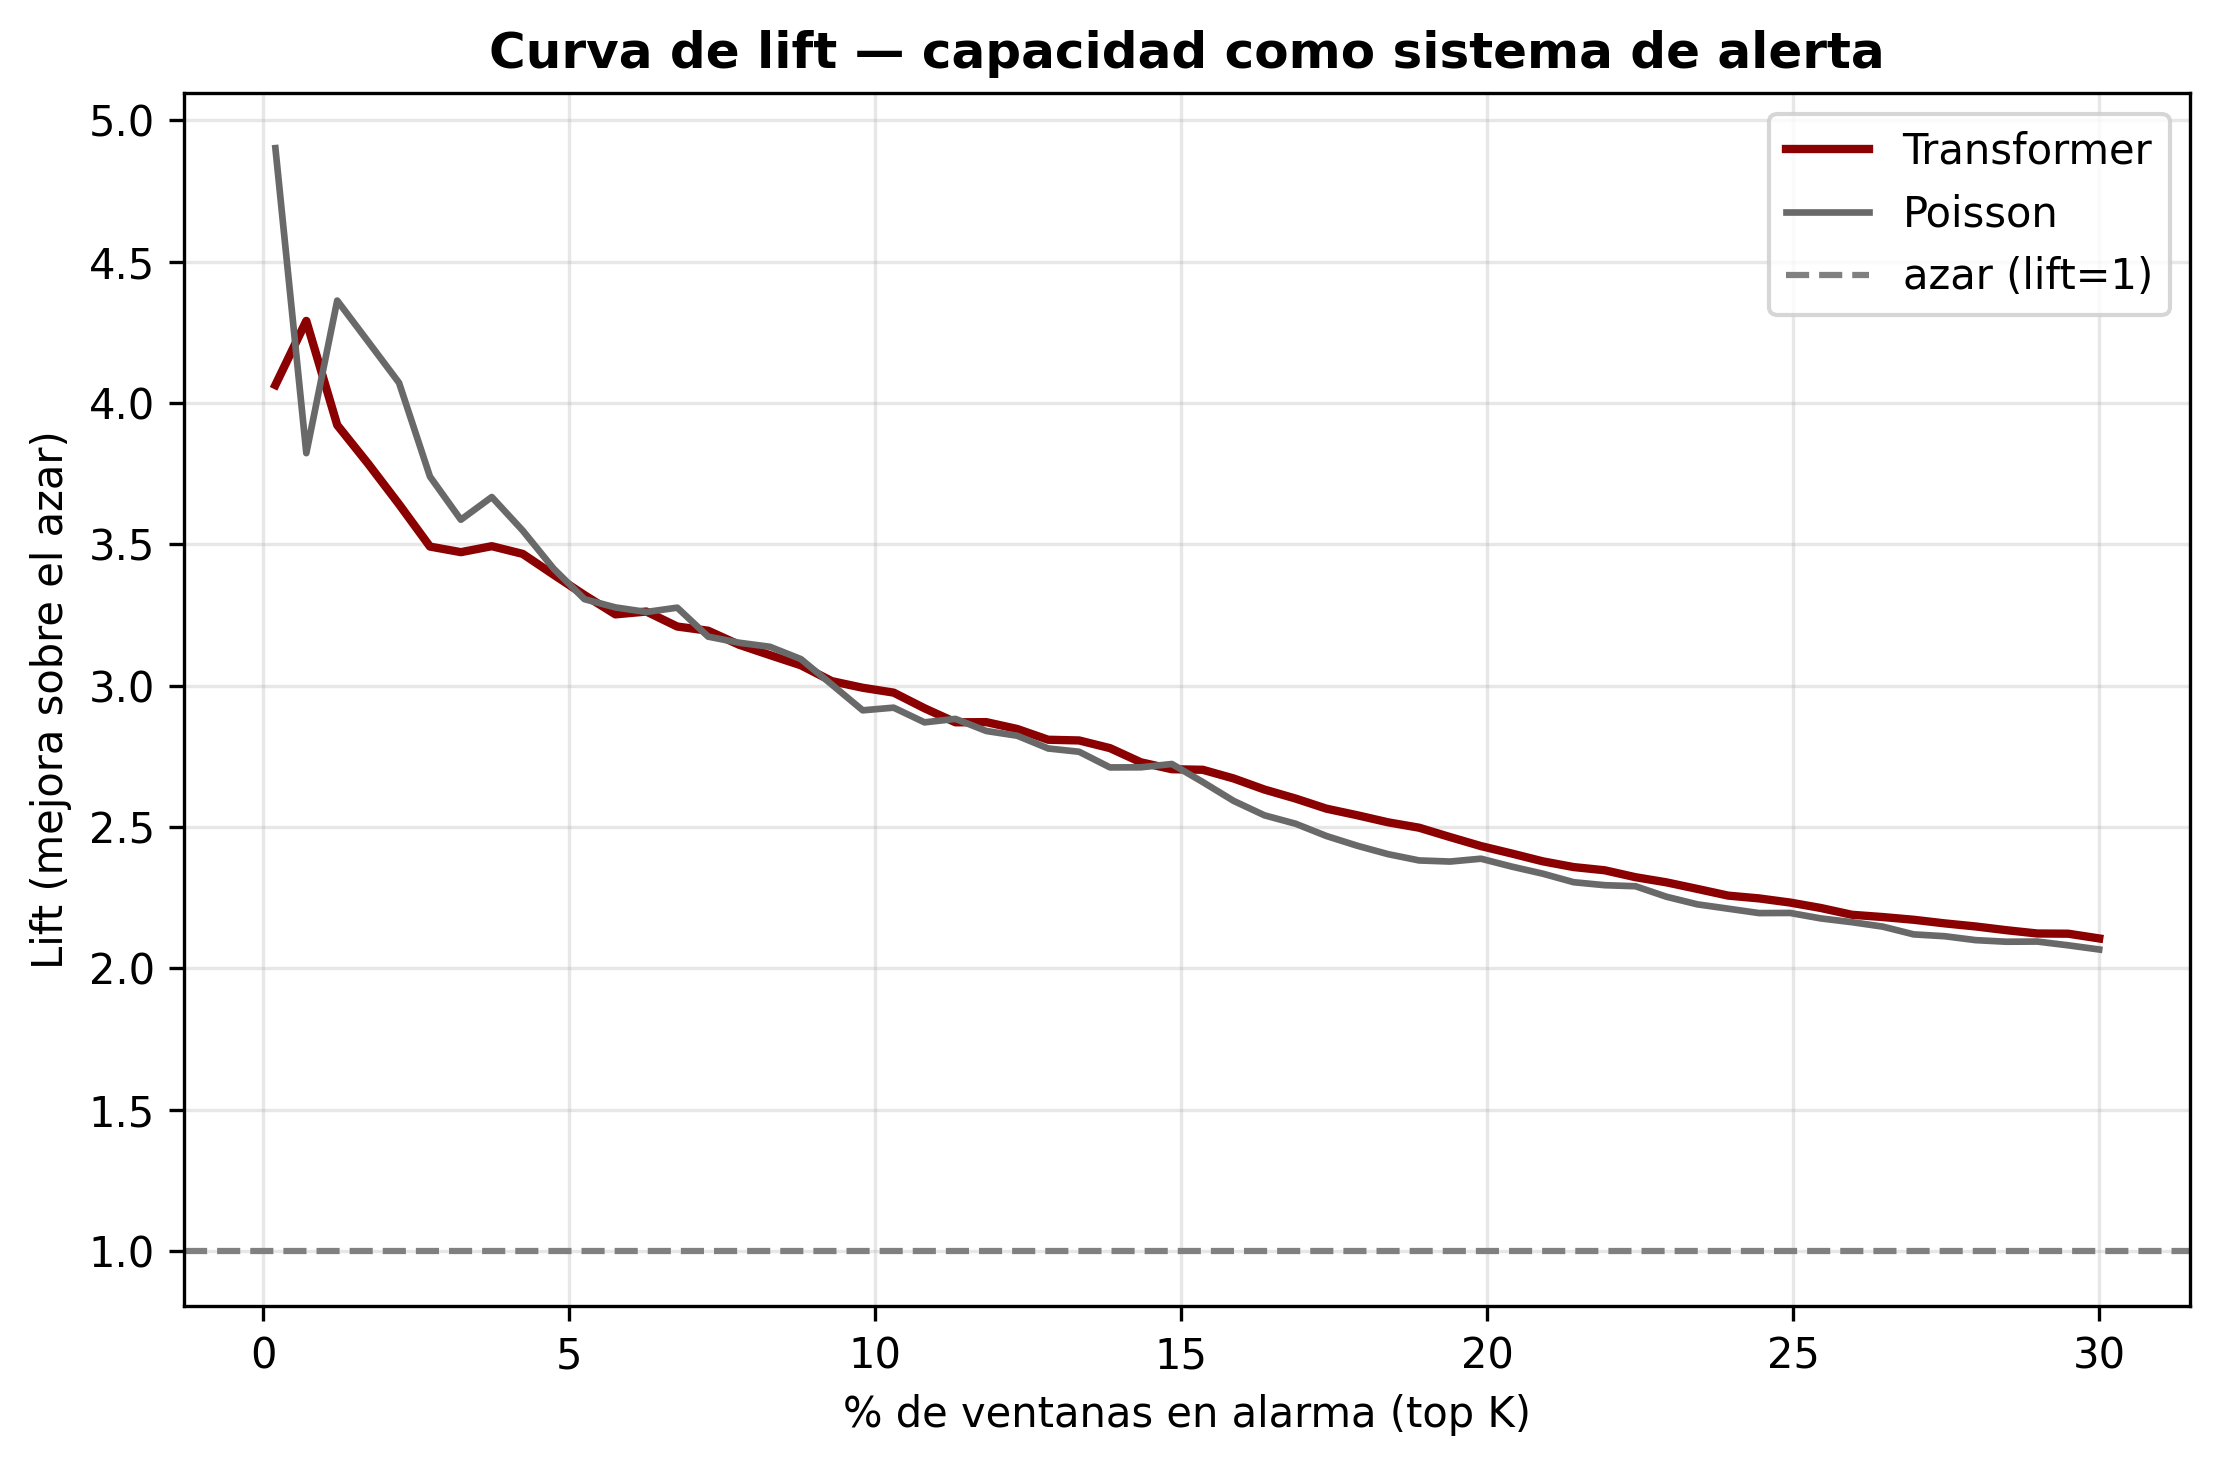
\includegraphics[width=0.74\textwidth]{figuras/05_lift_curve}
  \caption[Curva de \textit{lift} del Transformer]{\textbf{Curva de \textit{lift}.} Mejora respecto al azar al alertar del top \(K\)\,\% de mayor riesgo, en función de \(K\). Para alarmas muy concentradas (valores pequeños de \(K\)) la mejora supera cuatro veces el azar. Las curvas del Transformer y del Poisson son casi coincidentes.}
  \label{fig:lift}
\end{figure}

La lectura operativa es positiva: las alertas más confiadas del Transformer aciertan unas
\textbf{cuatro veces más que el azar} (\textit{lift} de 4.17 en el top 1\,\%). Concentrando las
alarmas en las zonas que el modelo considera más peligrosas se multiplica por cuatro la
probabilidad de acertar. La Figura~\ref{fig:pr} complementa este análisis con la curva
\textit{precision}-\textit{recall}, más adecuada que la ROC en un problema tan desbalanceado.
Estas cifras son prácticamente idénticas a las del Poisson, lo que vuelve a señalar que la
capacidad del sistema proviene de la cartografía espacial del peligro.

\begin{figure}[ht!]
  \centering
  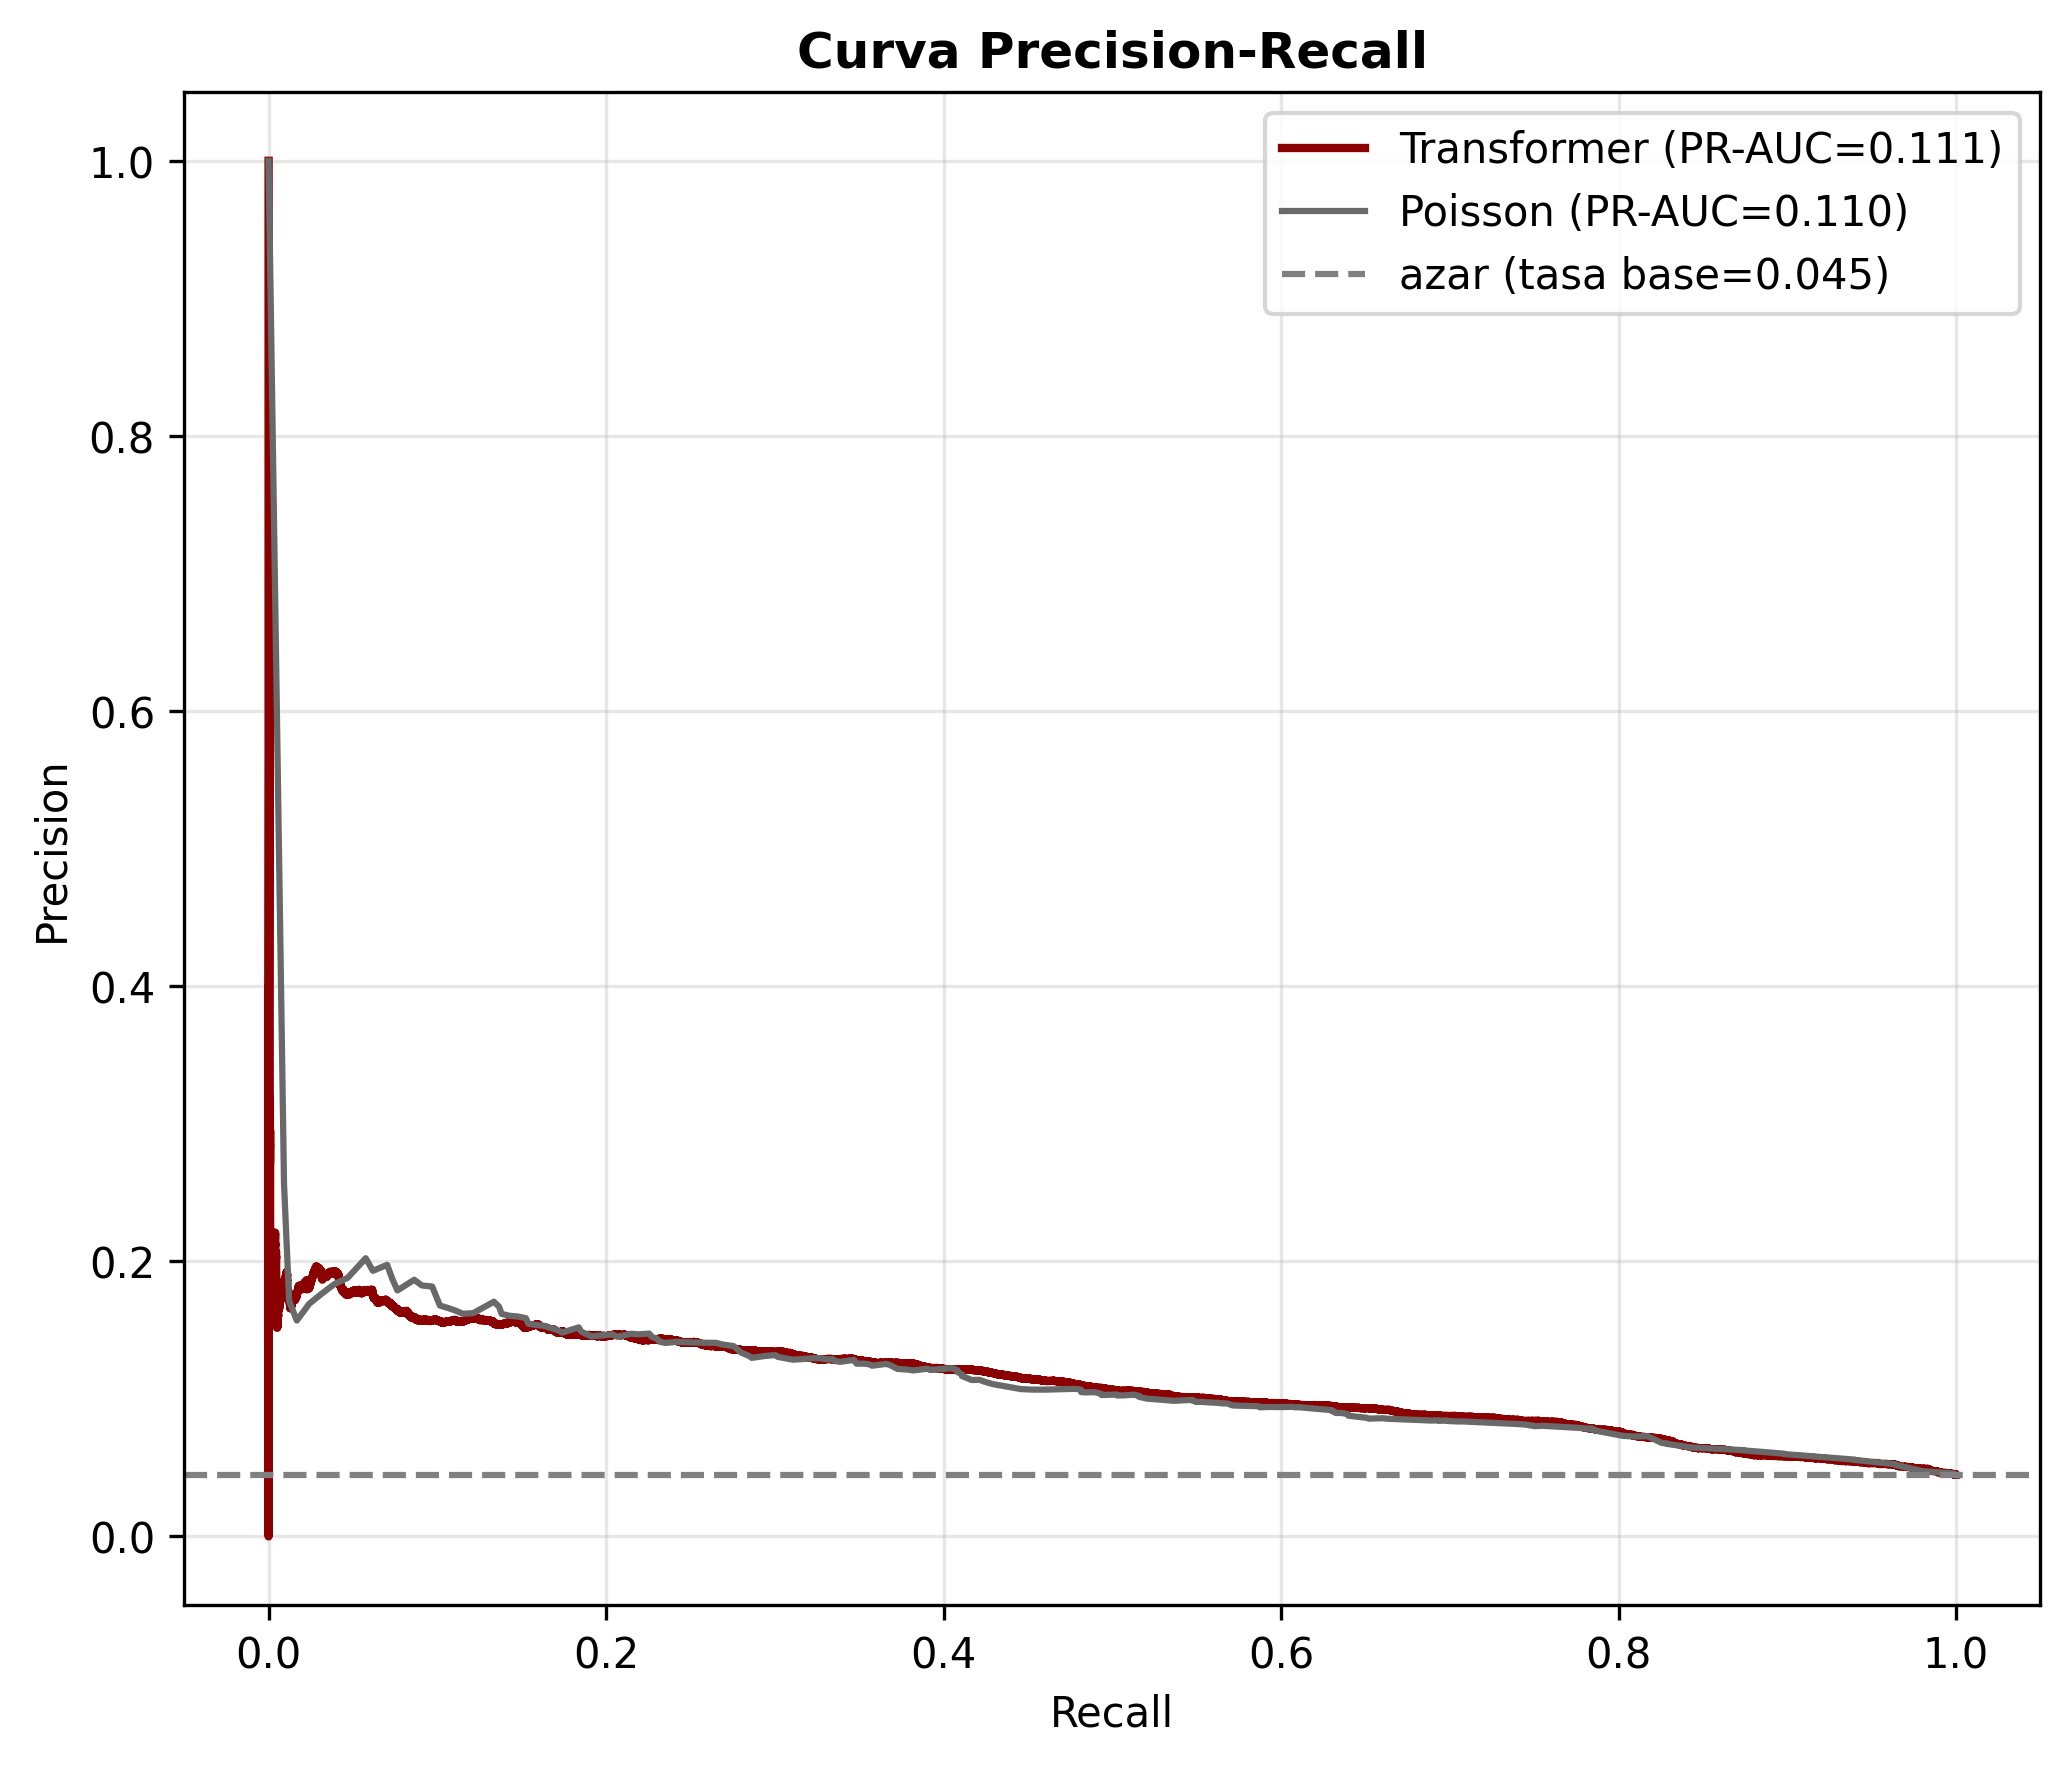
\includegraphics[width=0.66\textwidth]{figuras/05_pr_curve}
  \caption[Curva \textit{precision}-\textit{recall} del Transformer]{\textbf{Curva \textit{precision}-\textit{recall}} del Transformer frente al Poisson. La línea discontinua marca la tasa base, que es el nivel de un modelo aleatorio en esta métrica.}
  \label{fig:pr}
\end{figure}

Otra forma de comprobar que el modelo capta señal es observar cómo reparte sus probabilidades
entre los casos positivos y negativos. La Figura~\ref{fig:scoredist} superpone los dos
histogramas: el de las probabilidades asignadas a las ventanas que sí tuvieron un mainshock y el
de las que no. Aunque las dos distribuciones se solapan en gran medida --algo esperable en un
problema tan difícil y desbalanceado--, la distribución de los positivos está claramente
desplazada hacia probabilidades más altas, con una media mayor que la de los negativos. Es decir,
el modelo no asigna riesgo al azar: tiende a otorgar valores más elevados precisamente a las
ventanas que acaban siendo positivas, que es exactamente lo que sustenta el \textit{lift} y la
capacidad de alerta descritos arriba. El solapamiento, lejos de ser un defecto del modelo, refleja
la dificultad intrínseca del problema.

\begin{figure}[ht!]
  \centering
  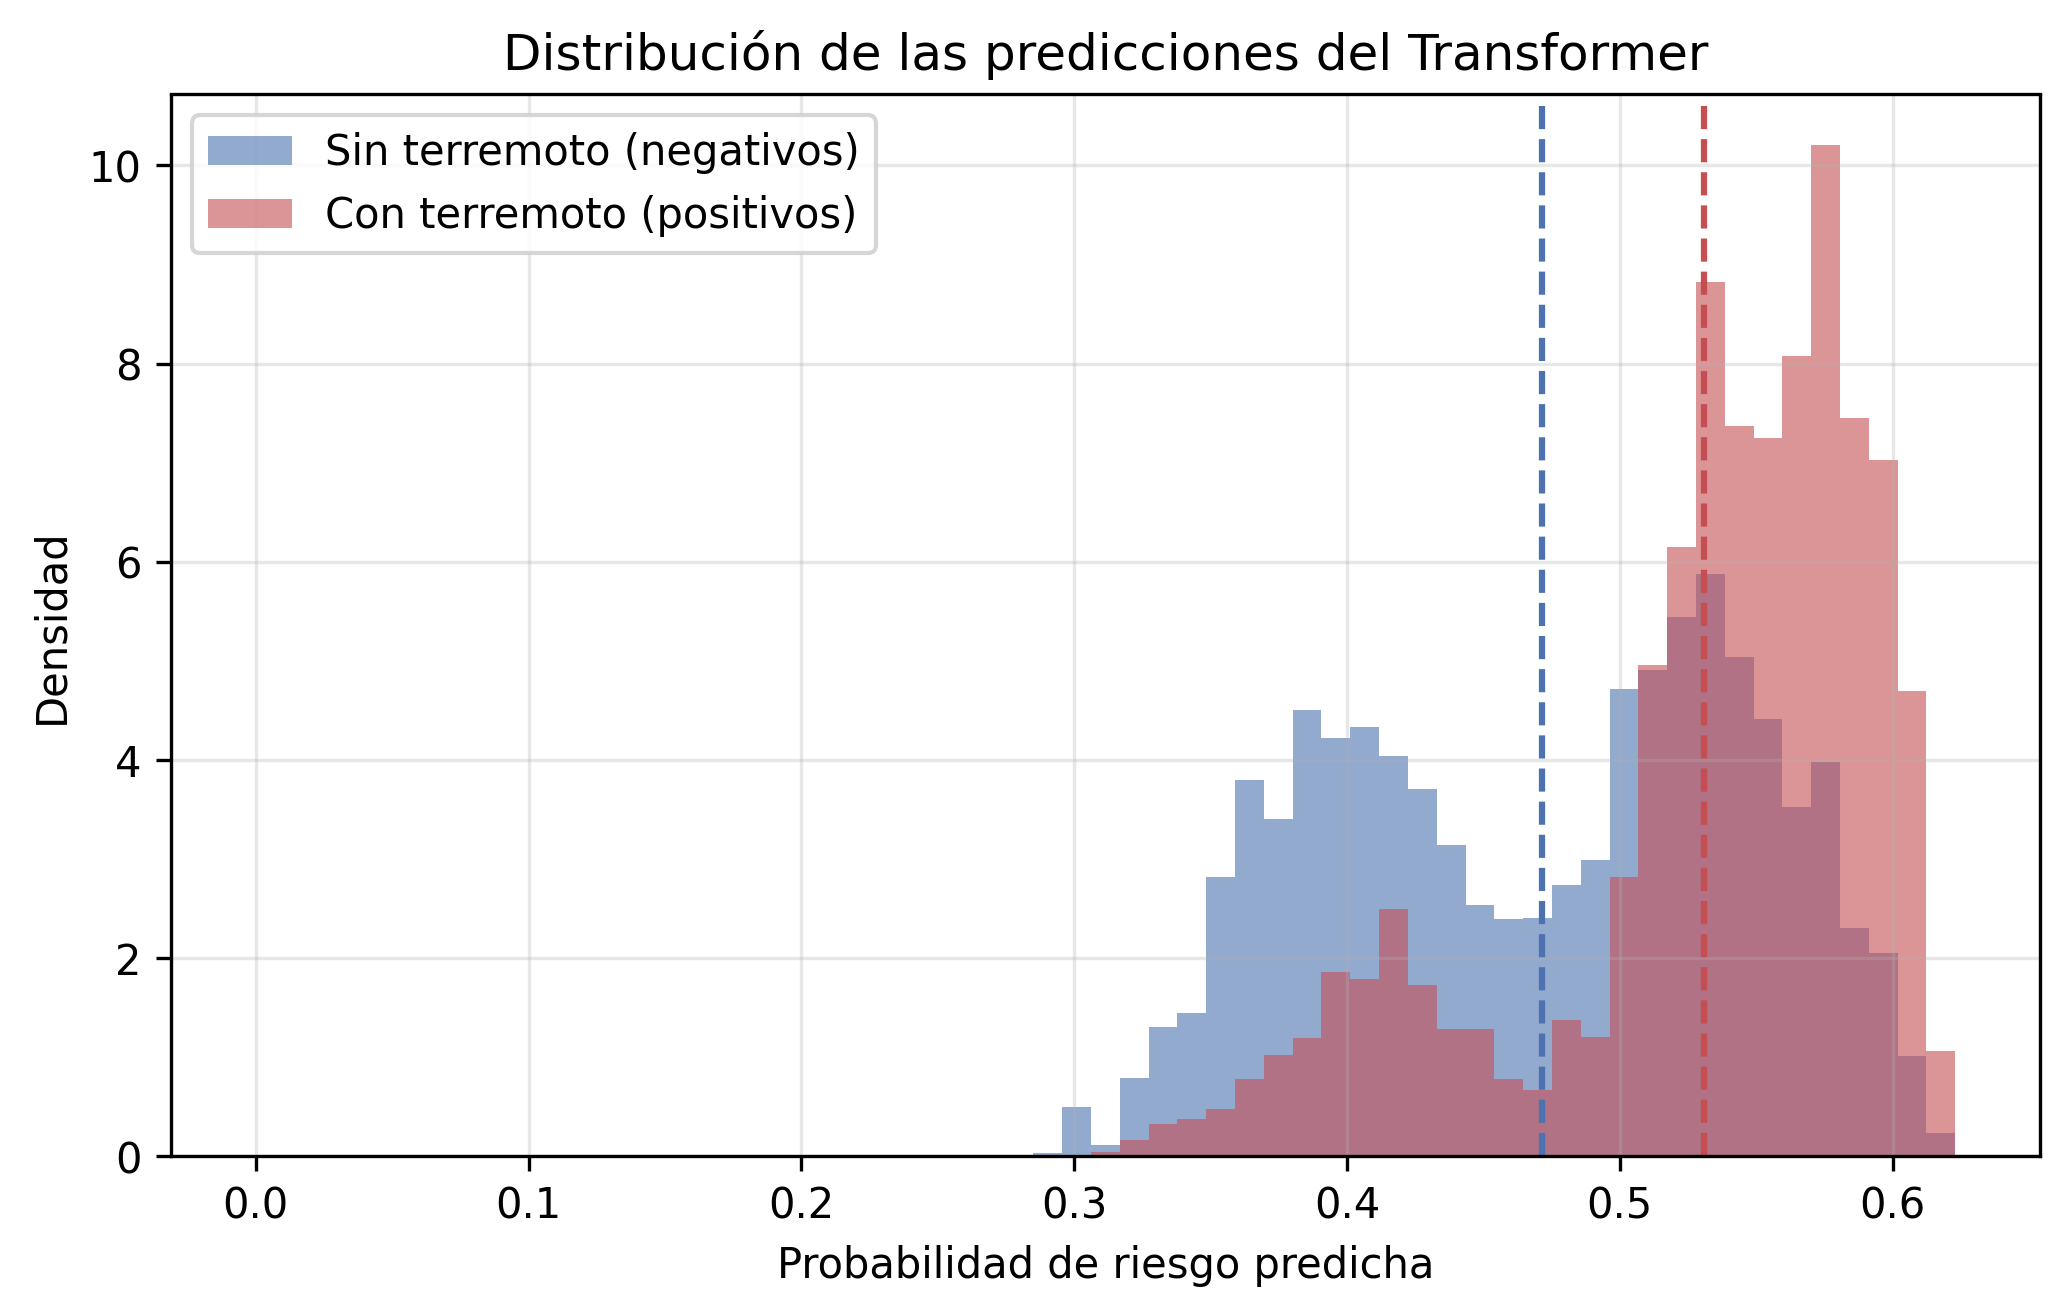
\includegraphics[width=0.72\textwidth]{figuras/05_score_dist}
  \caption[Distribución de las probabilidades predichas]{\textbf{Distribución de las probabilidades predichas por el Transformer}, separadas según el resultado real (con o sin mainshock). Las líneas discontinuas marcan las medias de cada grupo. La distribución de los positivos está desplazada hacia valores más altos, lo que muestra que el modelo concentra el riesgo en las ventanas correctas.}
  \label{fig:scoredist}
\end{figure}

\subsection{Análisis de la dimensión espacial y temporal}
\label{res-temporal}

El AUC global de 0.73 mezcla dos contribuciones de naturaleza muy distinta. Para separarlas se
recurre a la AUC temporal por celda, introducida en la Sección~\ref{md-metricas}. La idea es
preguntar, dentro de cada celda por separado, si el modelo distingue las ventanas de 30 días que
tendrán un terremoto de las que no. Un modelo que solo conociera la tasa media de cada celda
--como el Poisson-- obtendría exactamente 0.5 en esta métrica, porque asigna el mismo valor a
todas las ventanas de una misma celda.

La Figura~\ref{fig:auctemporal} muestra la distribución de la AUC temporal por celda para el
Transformer. La media se sitúa en torno a 0.50, prácticamente idéntica a la del Poisson. Esto
delimita con precisión dónde reside la información que aprovecha el sistema: \textbf{la capacidad
  discriminativa procede de la dimensión espacial} --es decir, de saber qué celdas son crónicamente
más activas-- mientras que la componente temporal a 30 días, una vez aislada, no añade
información por encima de la tasa base.

\begin{figure}[ht!]
  \centering
  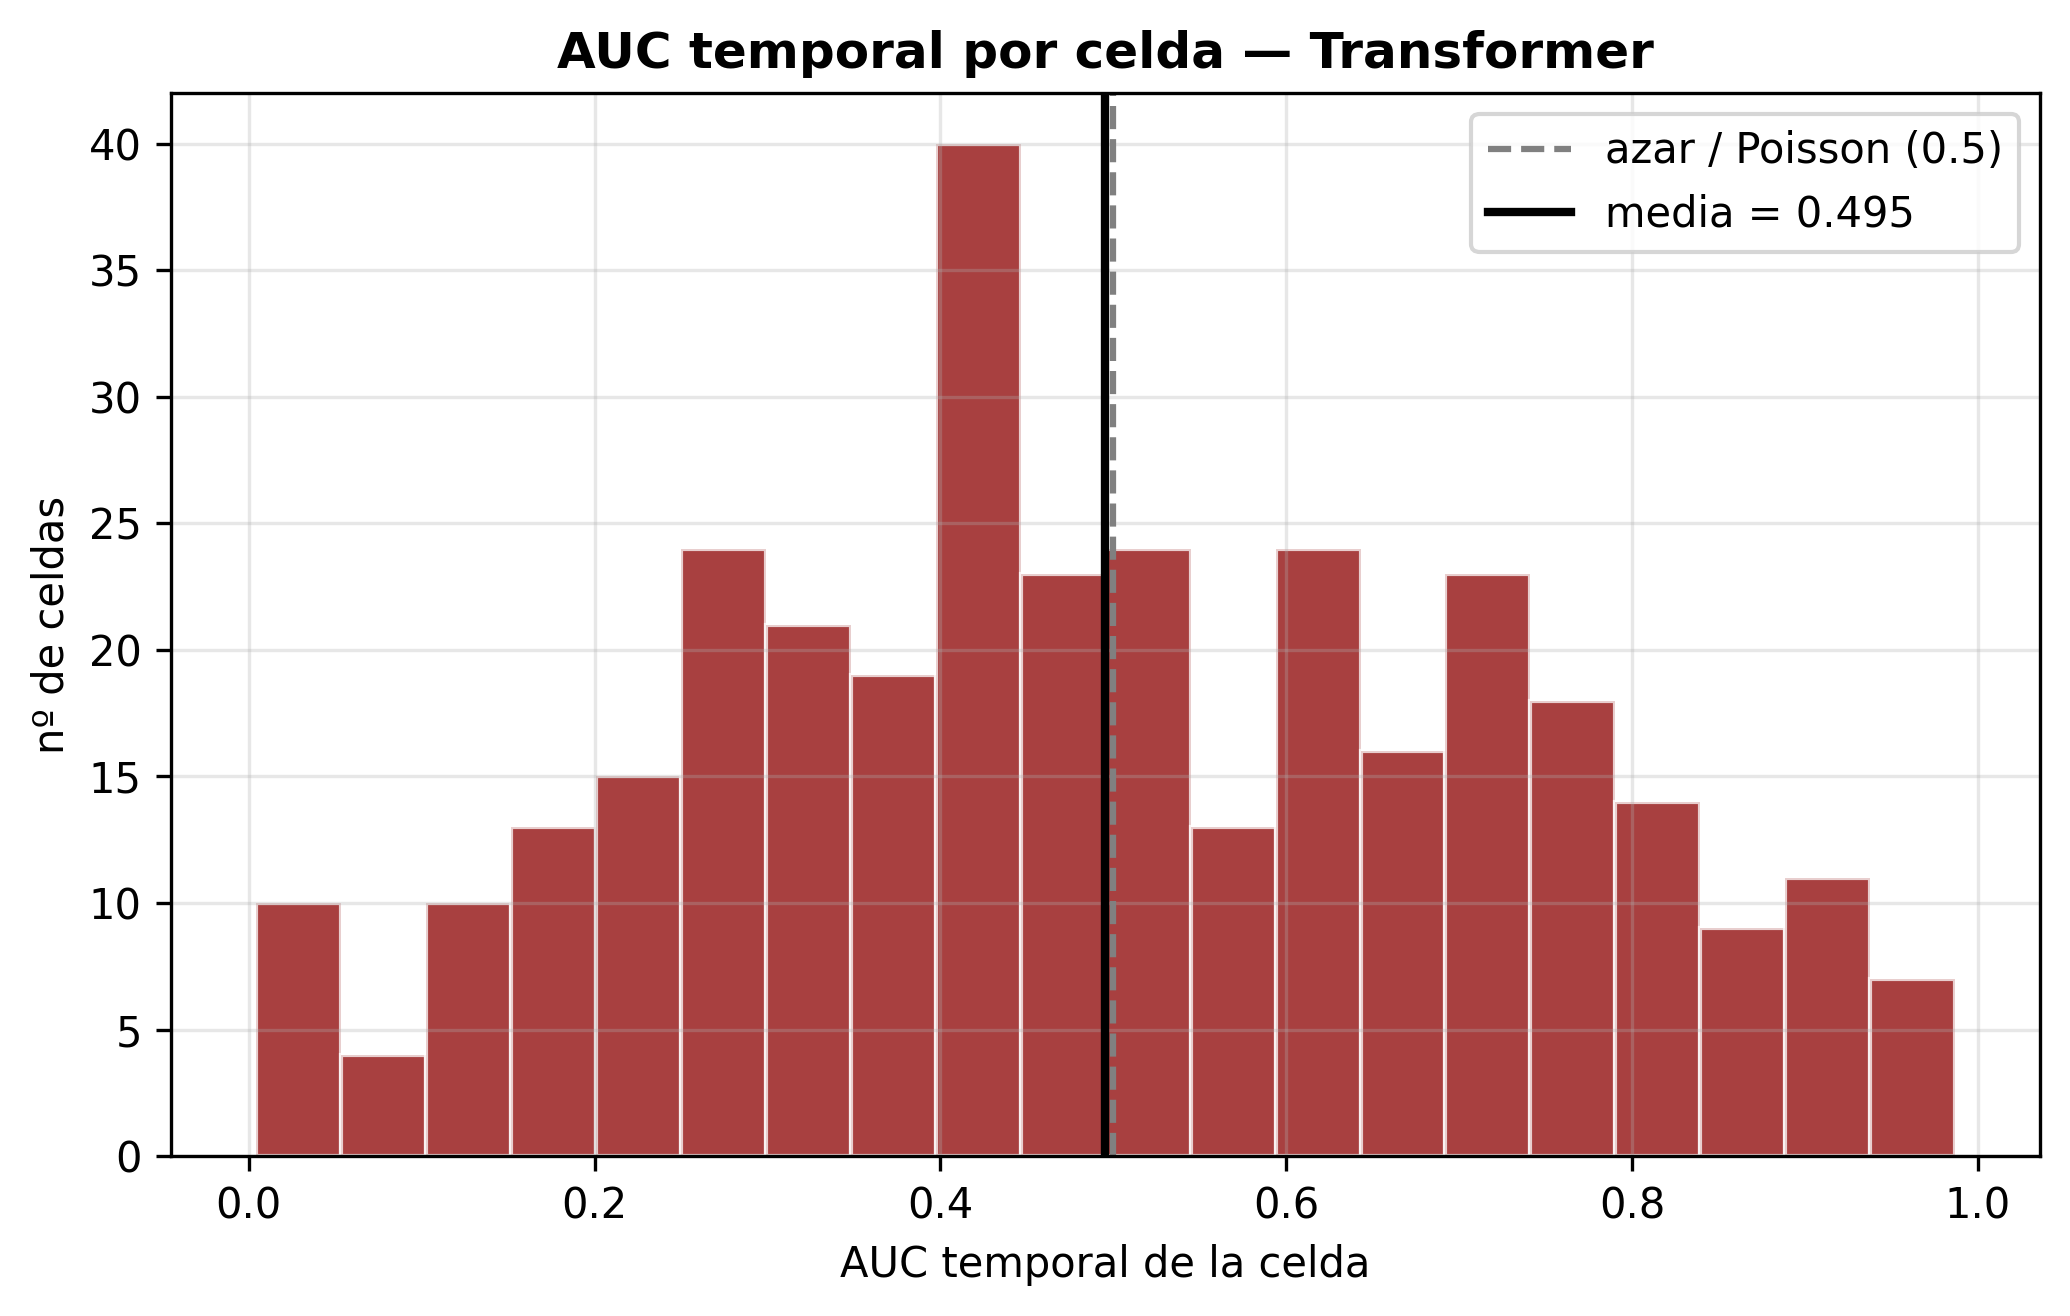
\includegraphics[width=0.74\textwidth]{figuras/05_auc_temporal}
  \caption[Distribución de la AUC temporal por celda]{\textbf{AUC temporal por celda} del Transformer. Cada barra cuenta las celdas con un valor dado. La media se sitúa cerca de 0.5, lo que indica que la capacidad de ordenar las ventanas temporales dentro de cada celda coincide con la de la climatología.}
  \label{fig:auctemporal}
\end{figure}

Este resultado es coherente con el consenso de la comunidad sismológica y constituye una de las
aportaciones del trabajo: gracias a una métrica diseñada específicamente, se localiza con
precisión la información predictiva. El sistema responde muy bien a la pregunta de \emph{dónde} es
más probable un terremoto --la estructura espacial de la sismicidad es estable y aprendible--
mientras que la pregunta de \emph{cuándo}, en un horizonte de 30 días y sobre el catálogo de
eventos, no encuentra una respuesta estadísticamente sólida. Esta distinción, lejos de ser una
limitación del método, es un hallazgo: indica que el valor del sistema está en la cartografía de
peligro espacial, que es justo lo que aprovecha la última fase.

Este mismo patrón se observa en la red de grafos, lo que confirma que no es una particularidad
del Transformer sino una propiedad del problema. La Figura~\ref{fig:gnncomp} reúne las curvas ROC
y de Molchan de la GNN frente al Poisson y la distribución de su AUC temporal por celda. Las dos
primeras muestran un comportamiento muy parecido al del Transformer, y la tercera vuelve a
situarse en torno a 0.5. Es decir, ambos modelos espaciales coinciden tanto en lo que logran
(cartografía espacial) como en lo que no (anticipación temporal), lo que da solidez a la
conclusión.

\begin{figure}[ht!]
  \centering
  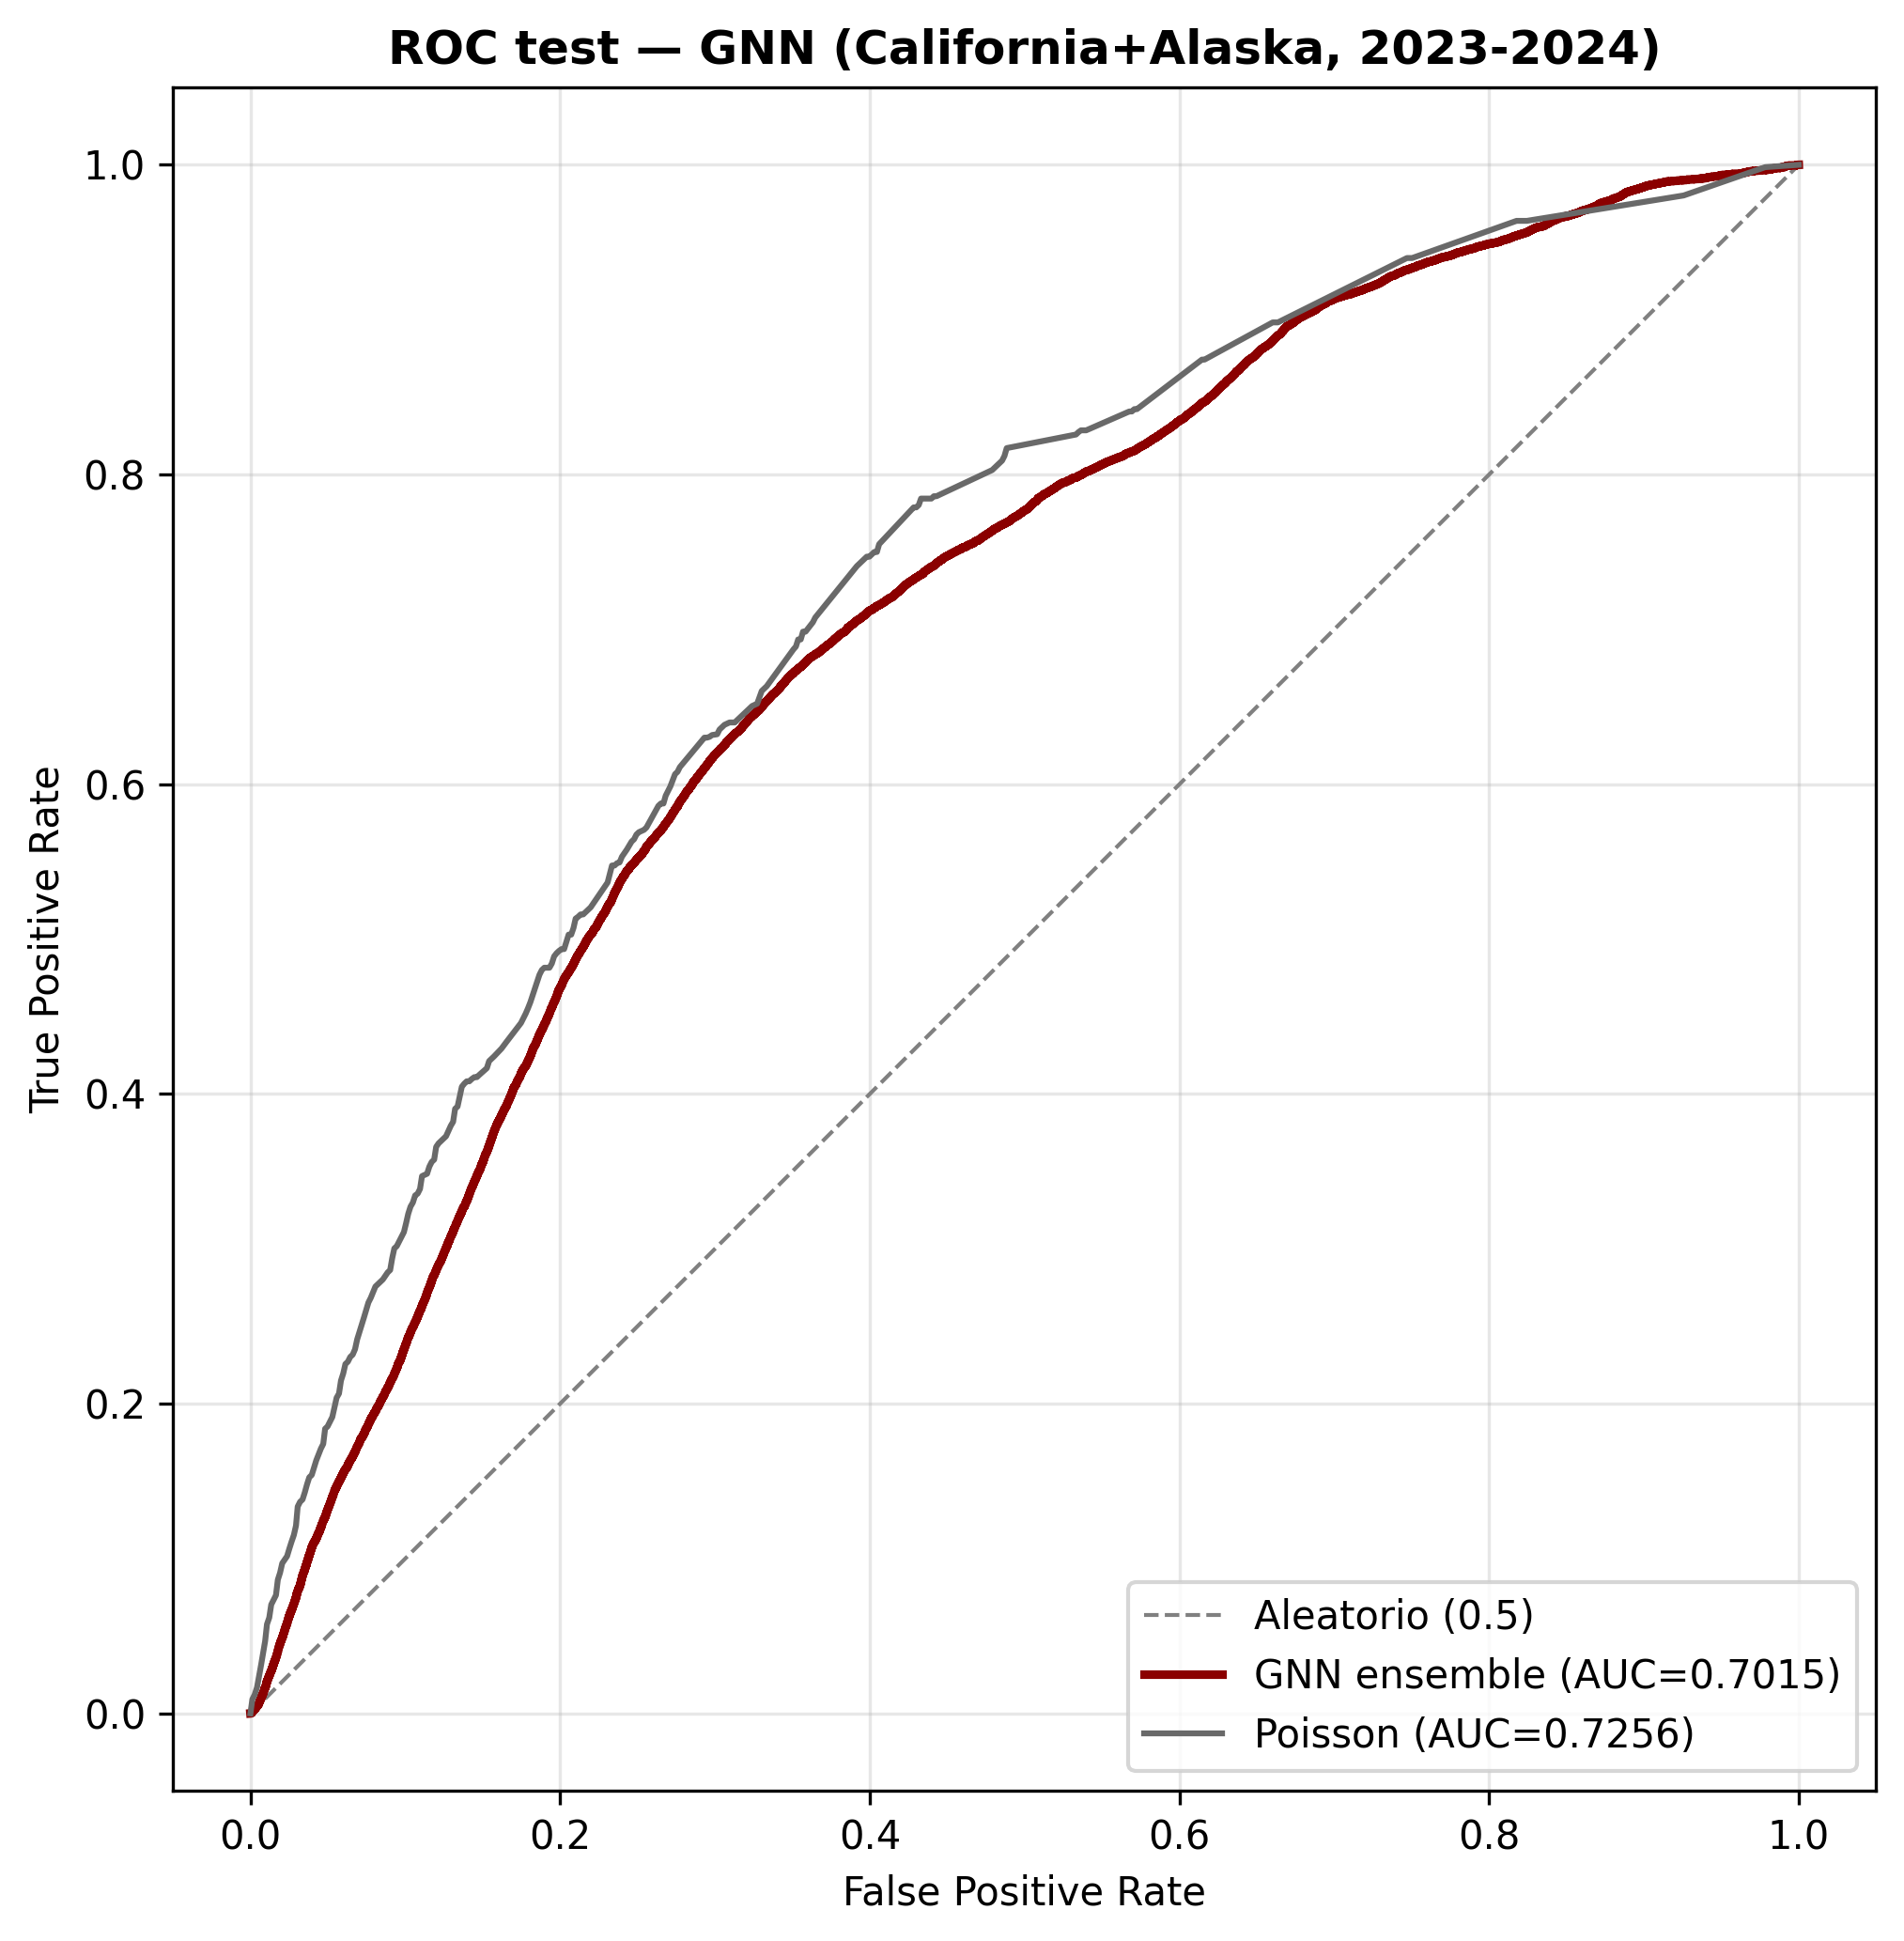
\includegraphics[width=0.49\textwidth]{figuras/04_roc_test}
  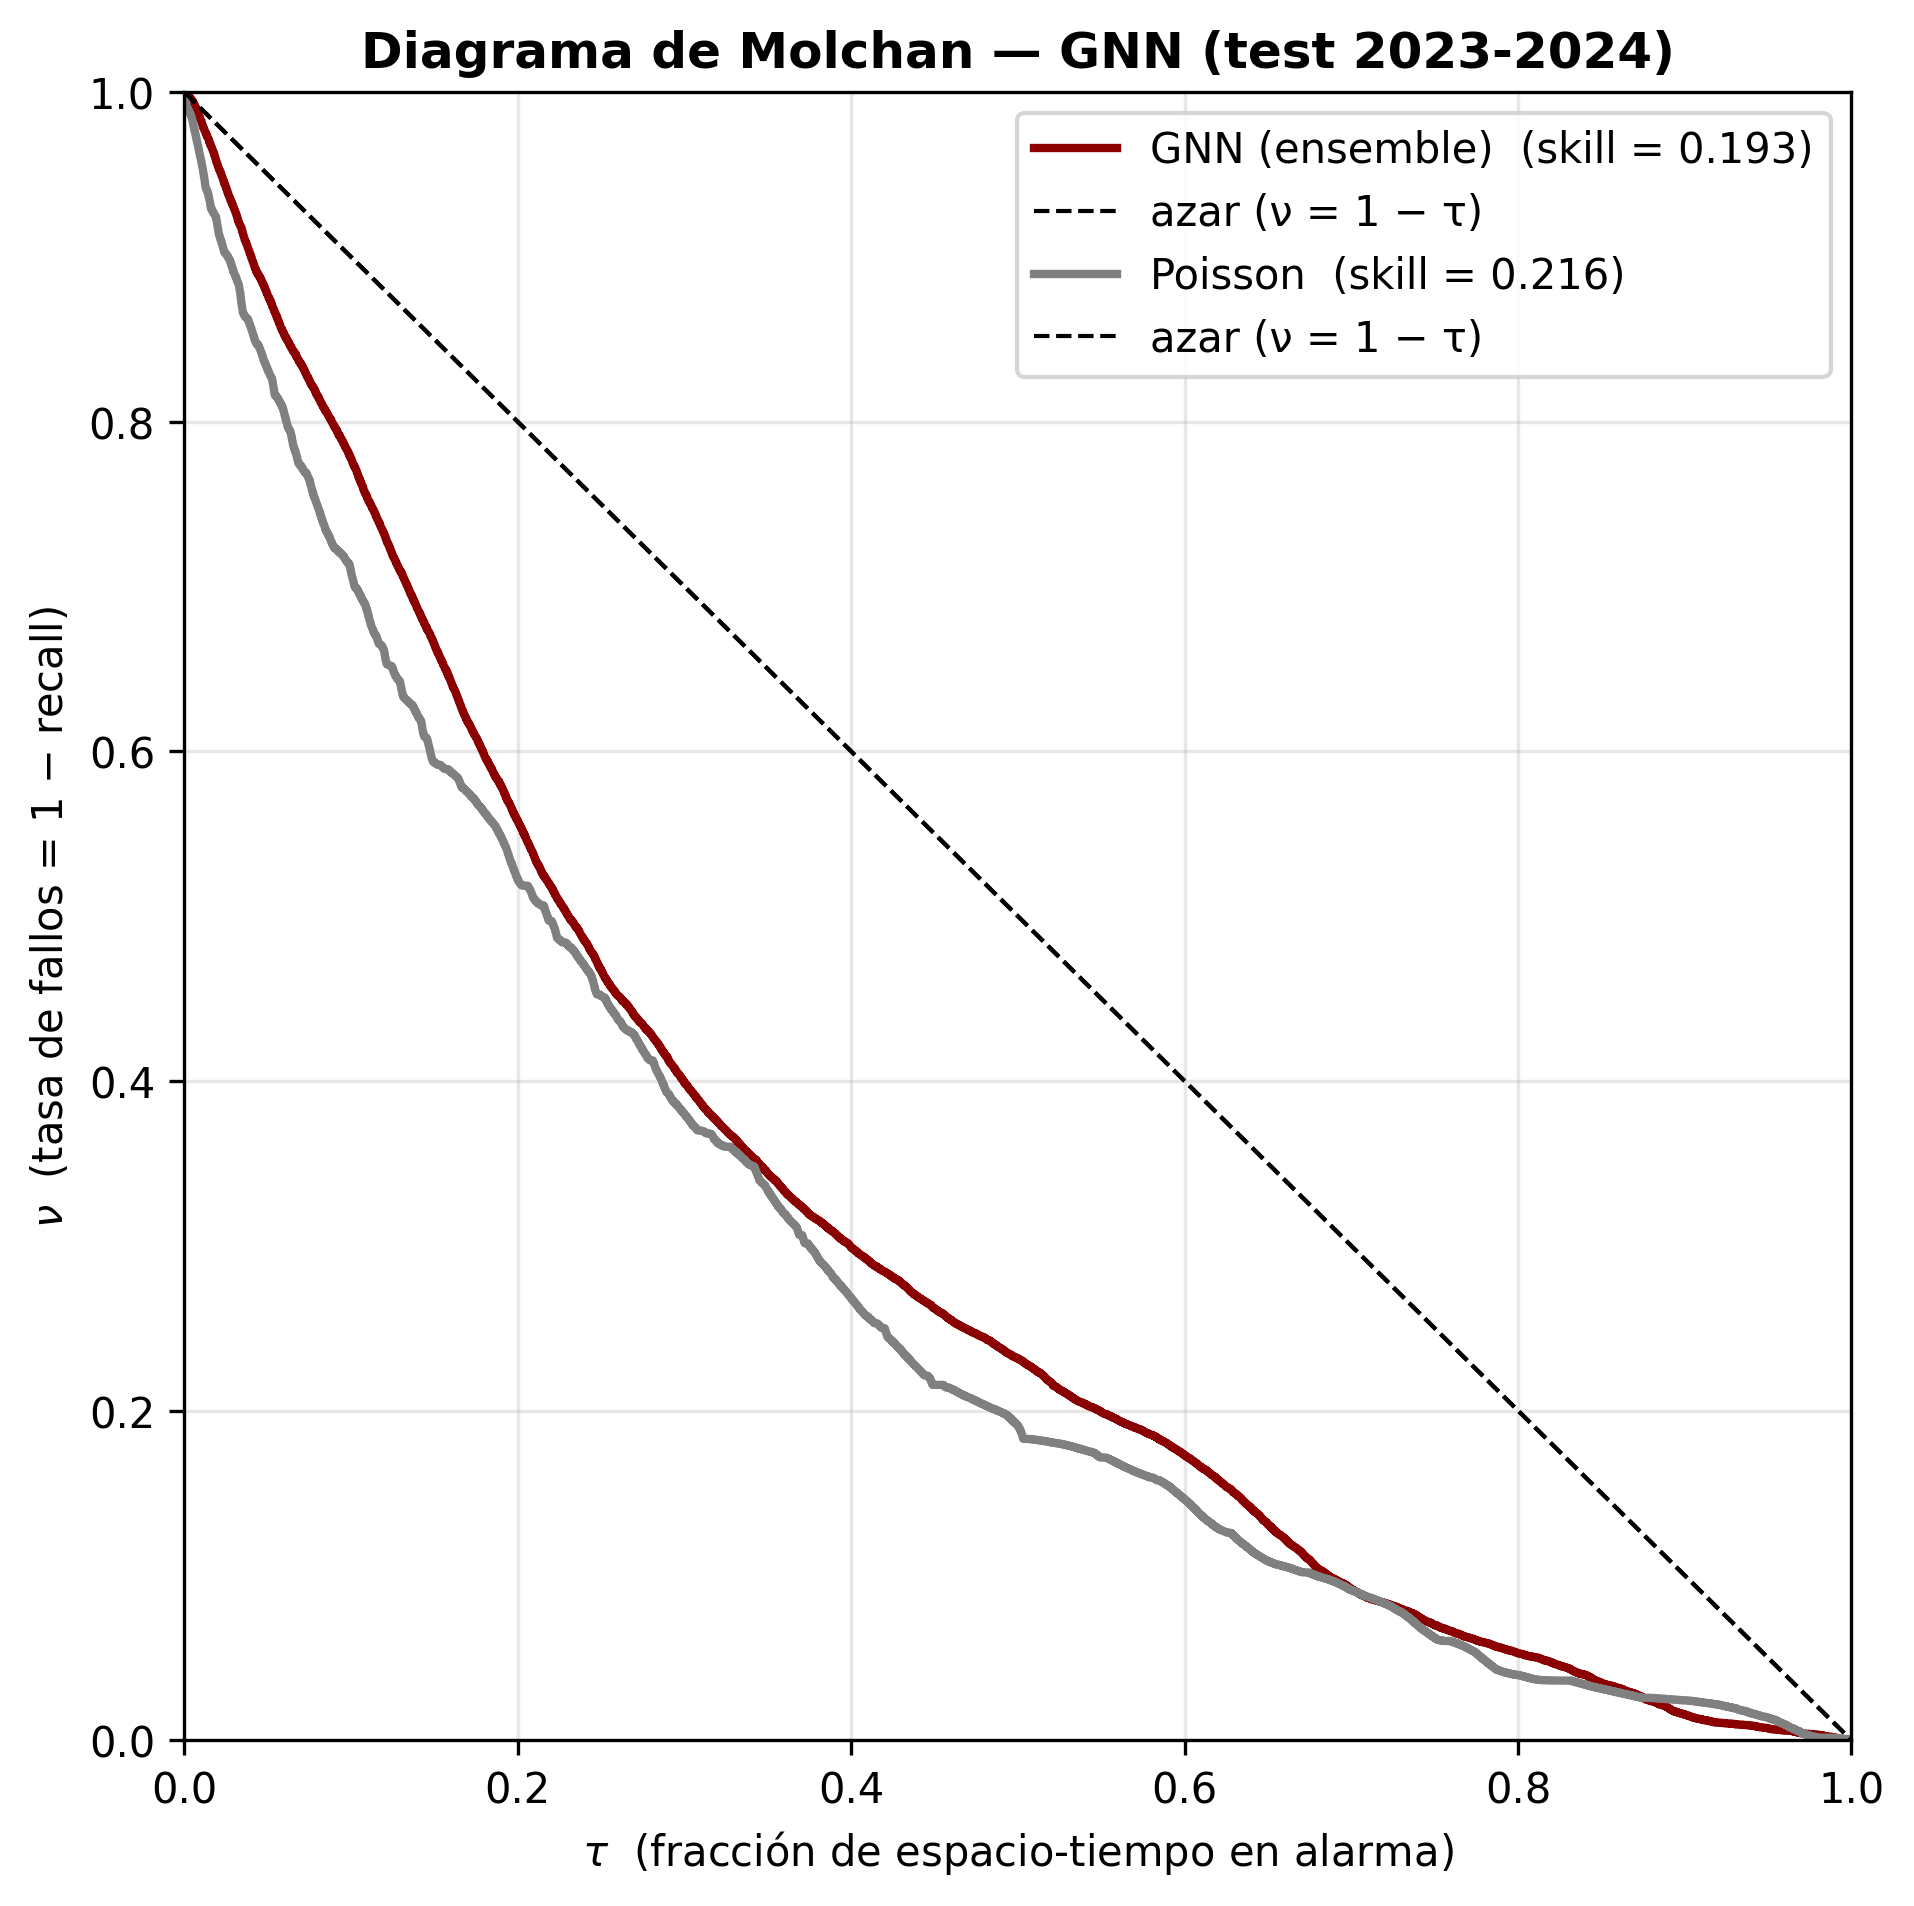
\includegraphics[width=0.49\textwidth]{figuras/04_molchan}\\[0.3cm]
  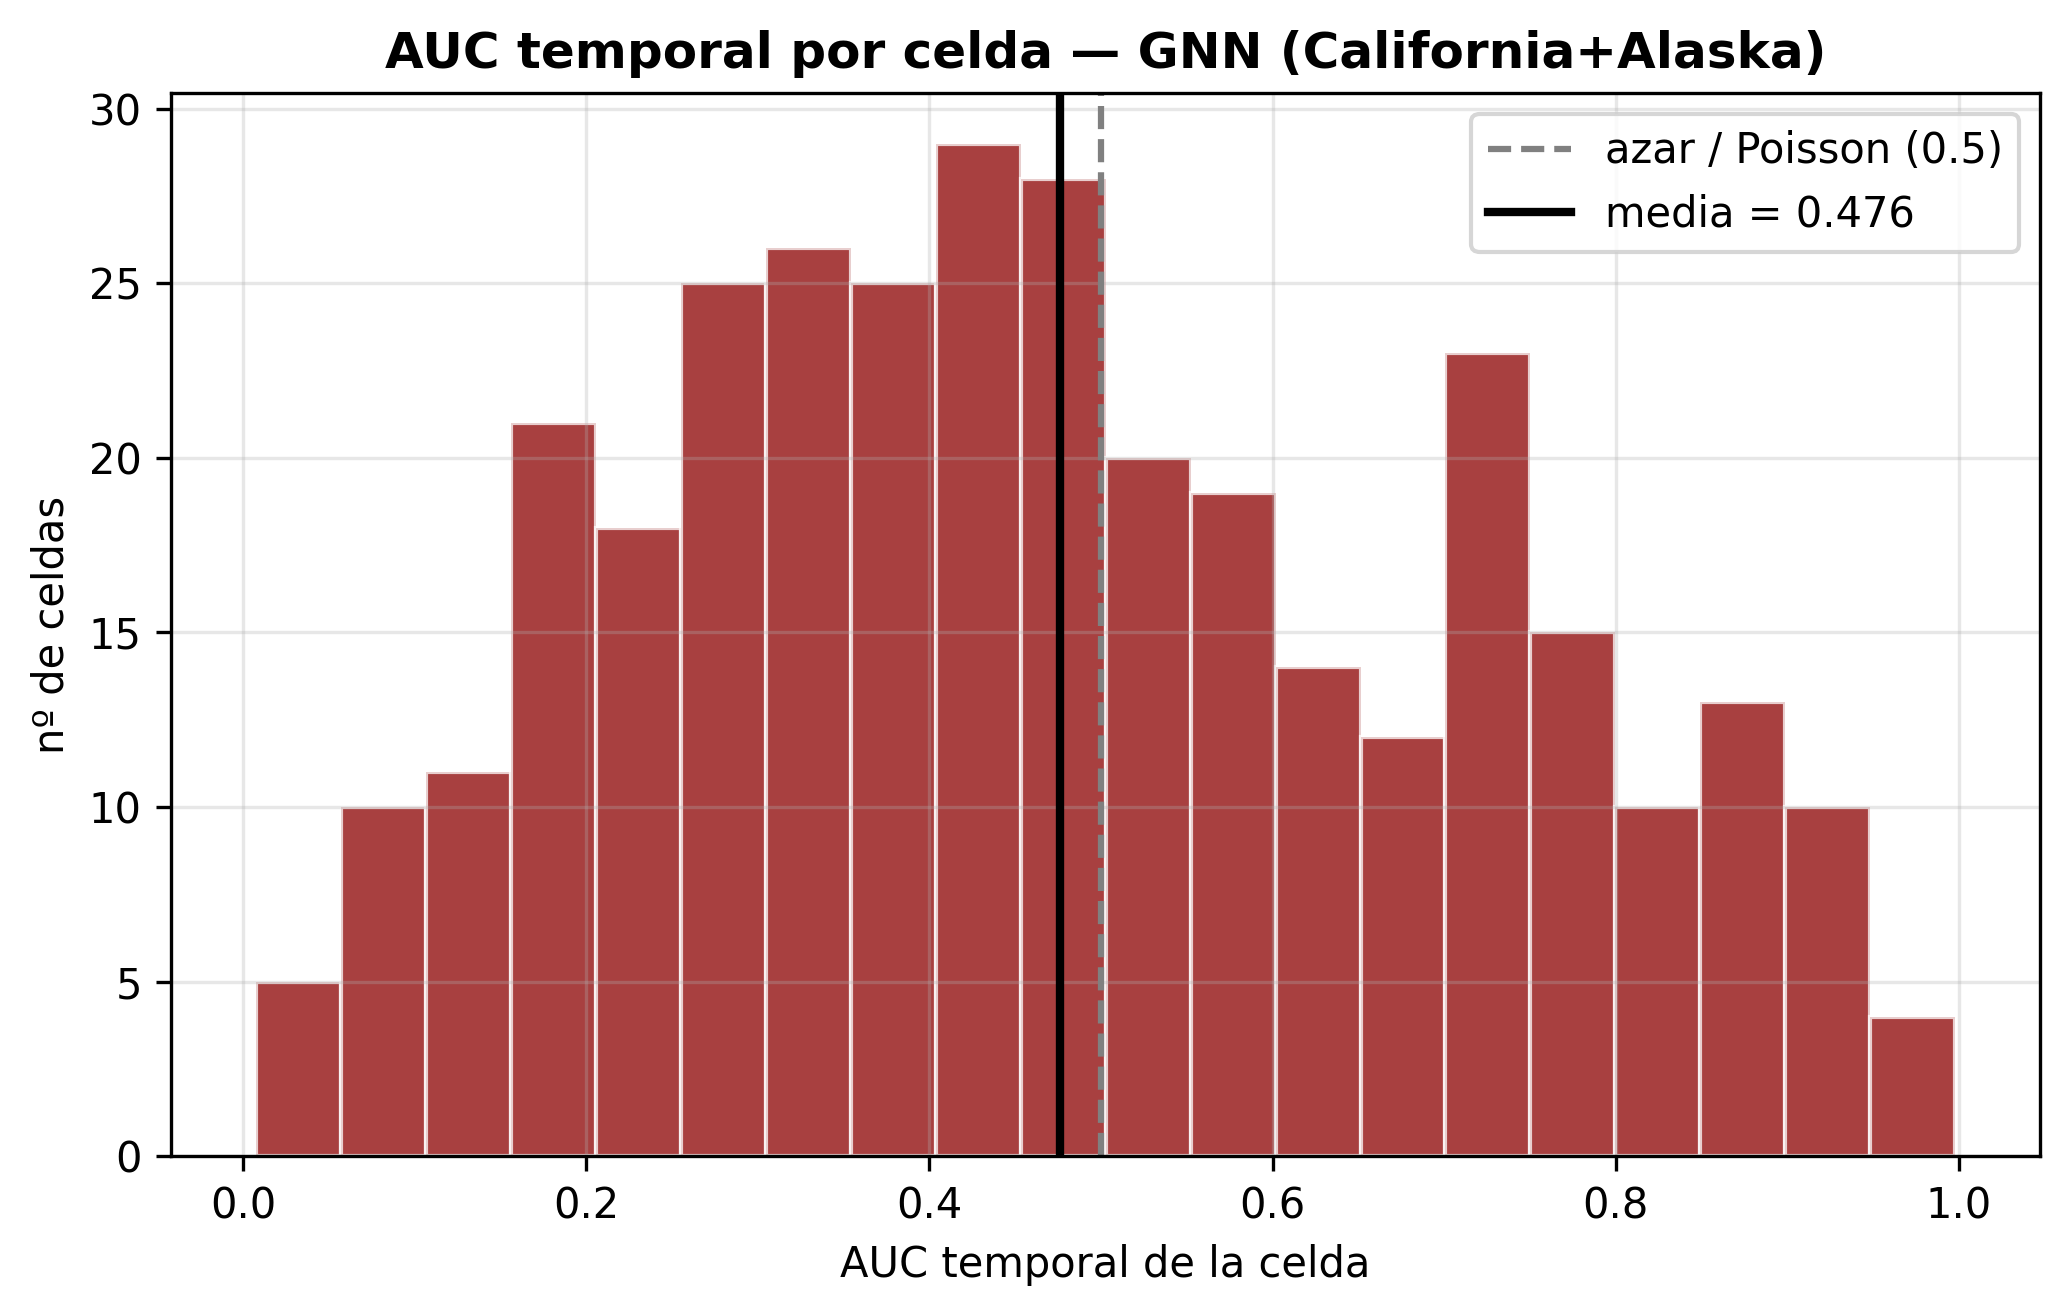
\includegraphics[width=0.6\textwidth]{figuras/04_auc_temporal}
  \caption[Resultados de la red de grafos]{\textbf{Resultados de la red de grafos (GNN).} Arriba: curva ROC (izquierda) y diagrama de Molchan (derecha) frente al Poisson. Abajo: distribución de la AUC temporal por celda, de nuevo centrada en torno a 0.5. El comportamiento reproduce el del Transformer, lo que confirma que este resultado se debe a la naturaleza del problema y no al tipo de arquitectura empleada.}
  \label{fig:gnncomp}
\end{figure}

\subsection{Estudios de ablación}
\label{res-ablations}

Para entender qué decisiones de diseño influyen en el resultado, y con qué dirección, se
realizaron varios estudios de ablación. La Tabla~\ref{tab:ablations} los resume. Cada uno
modifica un único elemento respecto al modelo de referencia y observa su efecto, prestando
especial atención a la AUC temporal por celda, que es la métrica que mide la señal predictiva
real.

Dos resultados de la tabla merecen comentario. Primero, al eliminar el \textit{declustering} el
AUC global sube, pero la AUC temporal por celda permanece en 0.509, prácticamente en el azar: la
mejora se explica íntegramente por la predictibilidad trivial de las réplicas, no por una
capacidad precursora nueva, lo que confirma que la decisión de declusterizar es metodológicamente
necesaria. Segundo, la adición de características diseñadas específicamente para captar anomalías
temporales por celda tampoco mejora el rendimiento del modelo. En conjunto, los estudios de ablación muestran que la conclusión
sobre la dimensión temporal es \textbf{robusta}: se mantiene al cambiar la arquitectura, la
ventana, el preprocesado del catálogo y las características. Esta robustez refuerza el valor del
hallazgo, porque descarta que se deba a una elección concreta de diseño.

\begin{table}[ht!]
  \centering
  \small
  \begin{tabular}{@{}lll@{}}
    \toprule
    \textbf{Variación}                    & \textbf{Efecto observado}               & \textbf{AUC temporal} \\
    \midrule
    Arquitectura GCN \(\to\) GAT          & mejora marginal, sin salto cualitativo  & 0.476                 \\
    \textit{Pooling} temporal completo    & ligera mejora del AUC global            & 0.495                 \\
    Ventana 30\,d \(\to\) 14\,d           & empeora el AUC global                   & 0.501                 \\
    Catálogo sin \textit{declustering}    & sube el AUC global (réplicas triviales) & 0.509                 \\
    Características de anomalía por celda & sin mejora apreciable                   & 0.483                 \\
    Filtro de profundidad \(\leq 70\)\,km & ligera bajada del AUC global            & 0.463                 \\
    \bottomrule
  \end{tabular}
  \caption[Resumen de los estudios de ablación]{\textbf{Estudios de ablación.} Cada fila modifica un elemento del modelo. La AUC temporal por celda se mantiene en el entorno de 0.5 (entre 0.46 y 0.51) en todas las ablaciones medidas, lo que indica que la conclusión sobre la dimensión temporal es robusta frente a estas variaciones.}
  \label{tab:ablations}
\end{table}

\subsection{Calibración y mapas de riesgo}
\label{res-gp}

La última fase transforma las predicciones espaciales en mapas de riesgo. Antes de la
interpolación es necesario calibrar las probabilidades del modelo, porque la ponderación de clase
usada en el entrenamiento las infla. La Figura~\ref{fig:calibracion} muestra la curva de
fiabilidad antes y después de la calibración isotónica, validada sobre una mitad del test
independiente de la usada para ajustar la calibración, de modo que la comparación no es
circular. El \textit{Brier score} mejora de 0.28 a 0.09, una reducción de dos tercios: tras
la calibración, las probabilidades del mapa reflejan frecuencias de ocurrencia reales, lo que es
esencial para un producto orientado a la toma de decisiones, ya que un mapa que sobreestimara el
riesgo generaría fatiga de alarma.

\begin{figure}[ht!]
  \centering
  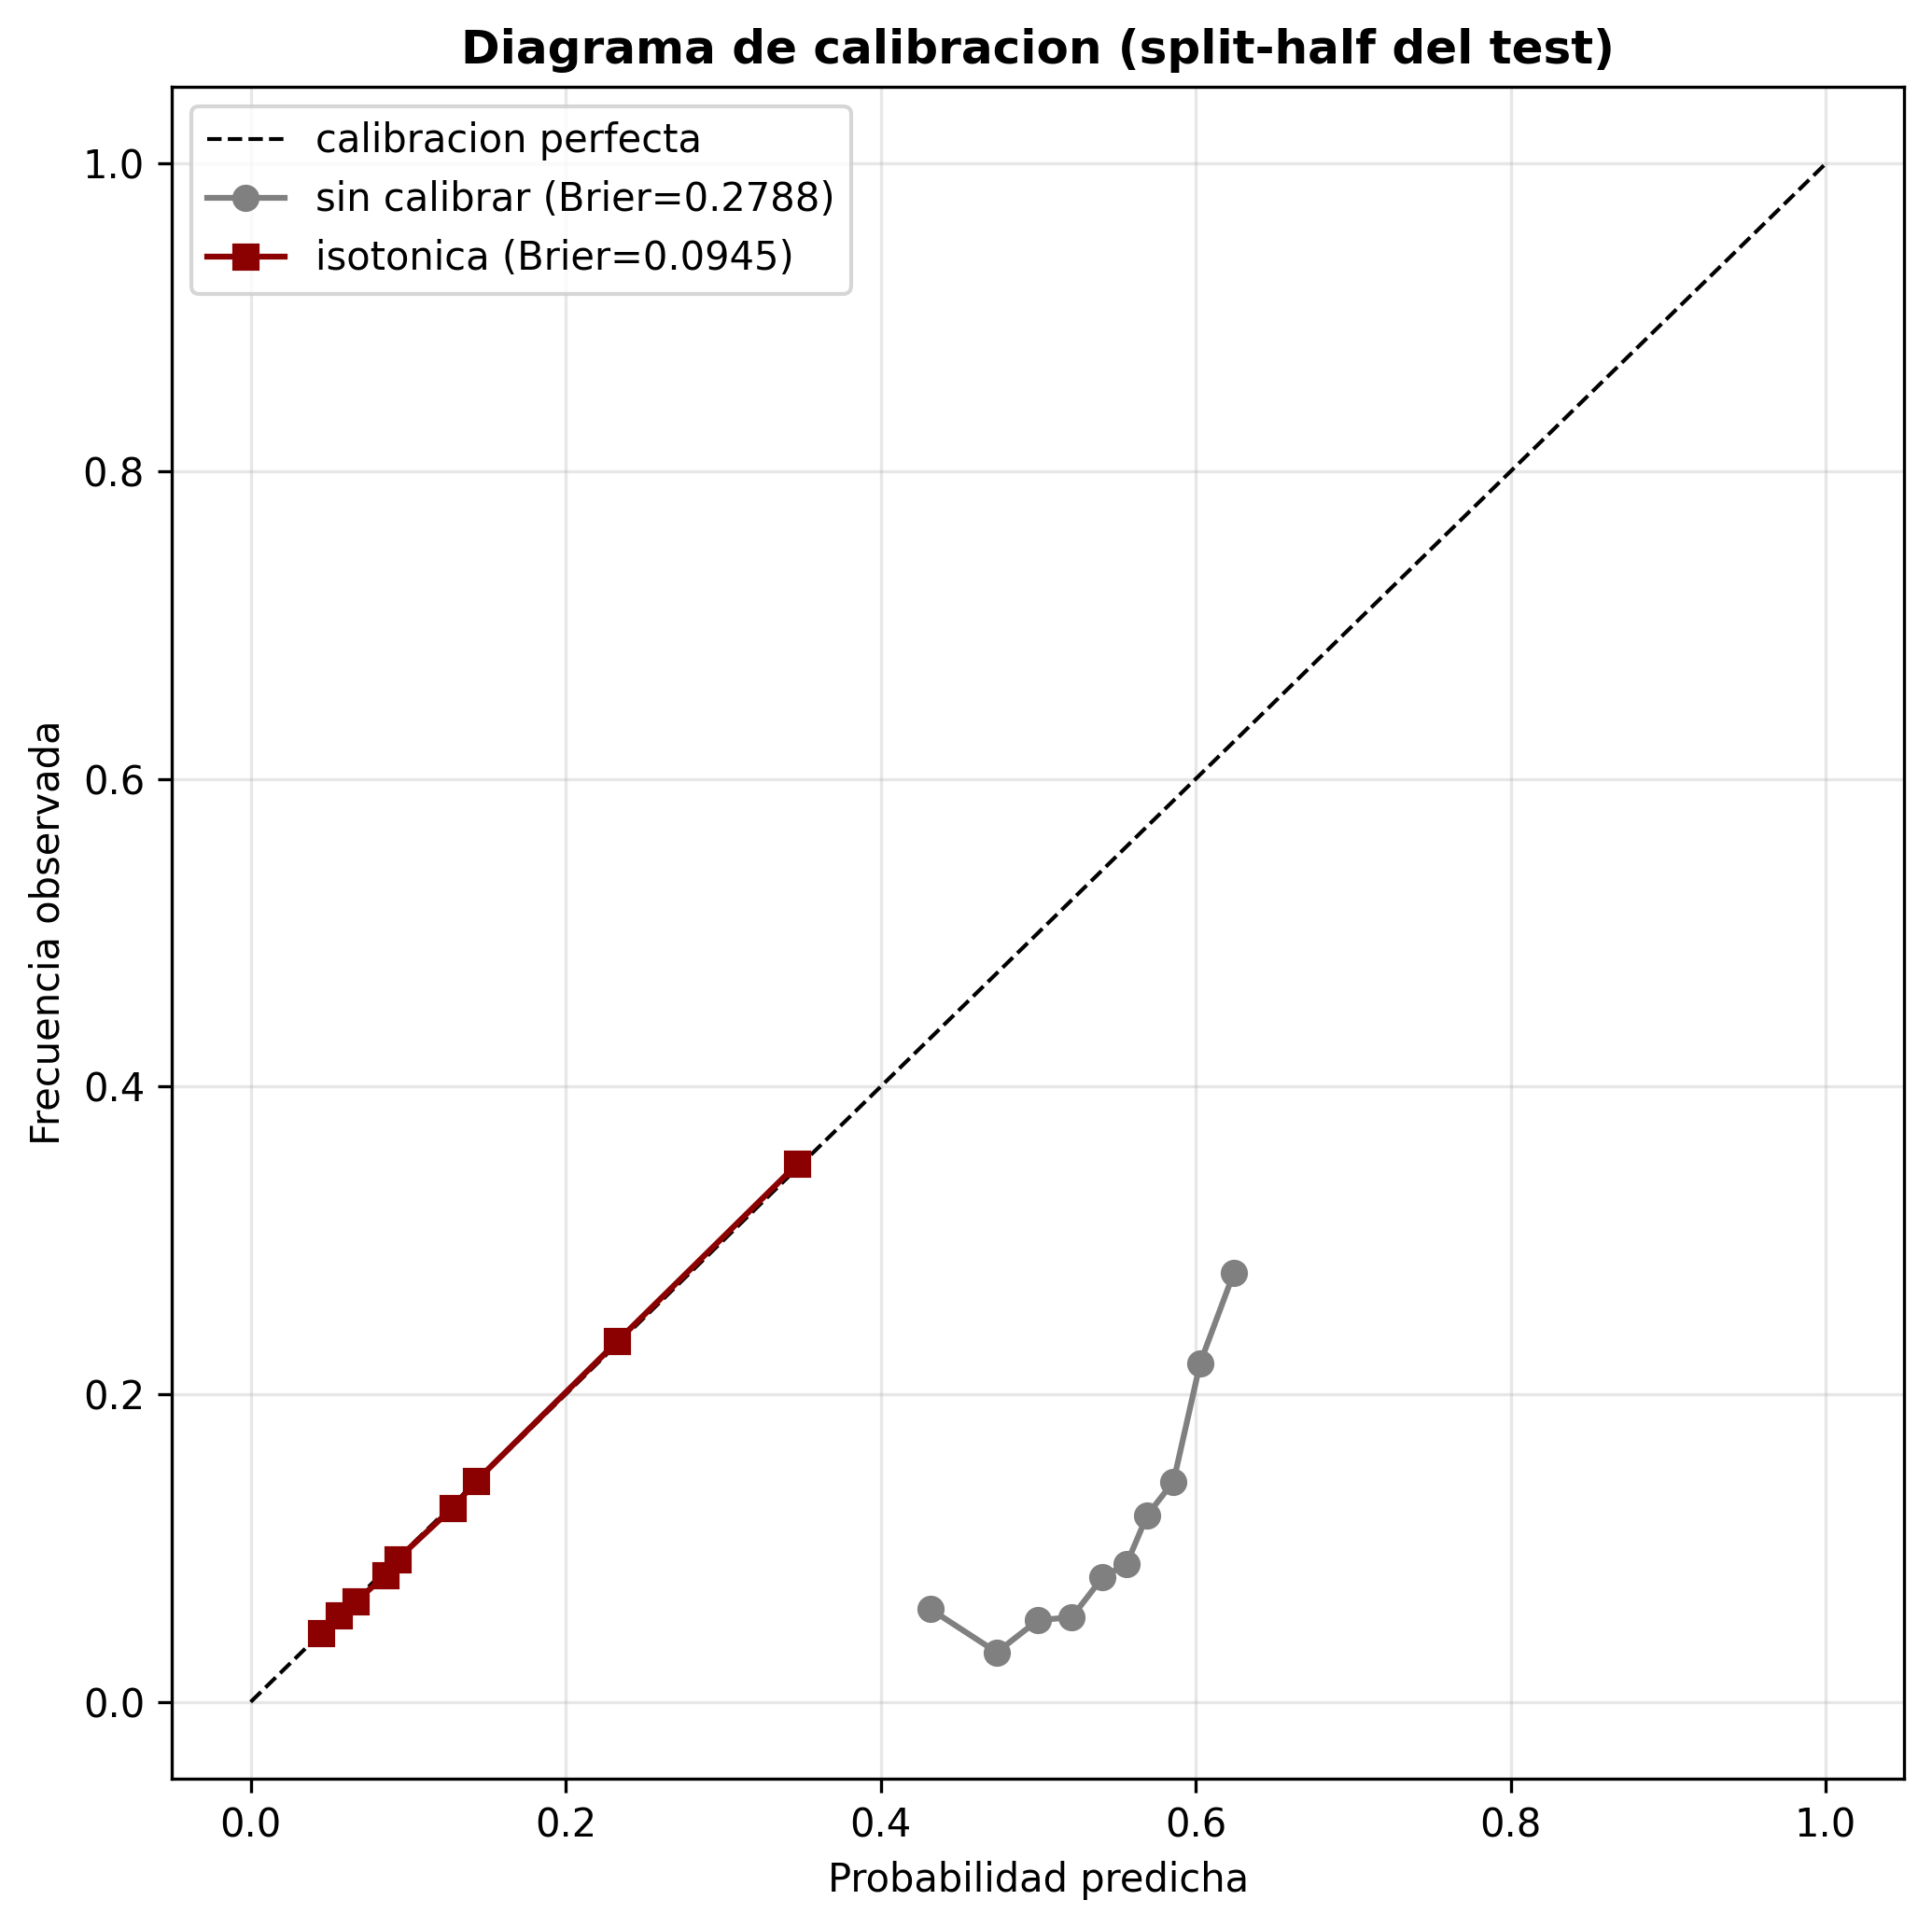
\includegraphics[width=0.6\textwidth]{figuras/06_calibracion}
  \caption[Curva de calibración y \textit{Brier score}]{\textbf{Diagrama de calibración.} Probabilidad predicha frente a frecuencia observada, antes (gris) y después (rojo) de la calibración isotónica. La calibración acerca las predicciones a la diagonal ideal y reduce el \textit{Brier score} de 0.28 a 0.09.}
  \label{fig:calibracion}
\end{figure}

Las Figuras~\ref{fig:mapacali} y~\ref{fig:mapaalaska} presentan los mapas de riesgo y de
incertidumbre obtenidos con el proceso gaussiano para California y Alaska. El mapa de riesgo
(izquierda) muestra una superficie continua que concentra el riesgo a lo largo de las grandes
estructuras tectónicas. El mapa de incertidumbre (derecha) es bajo cerca de las celdas con datos
y crece en las zonas sin sismicidad registrada, donde el modelo extrapola; es decir, la confianza
del mapa sigue a la disponibilidad de datos, como cabe esperar de un método bayesiano. Las
estrellas marcan los mainshocks reales del periodo de test, que tienden a caer en las zonas de
riesgo alto.

\begin{figure}[ht!]
  \centering
  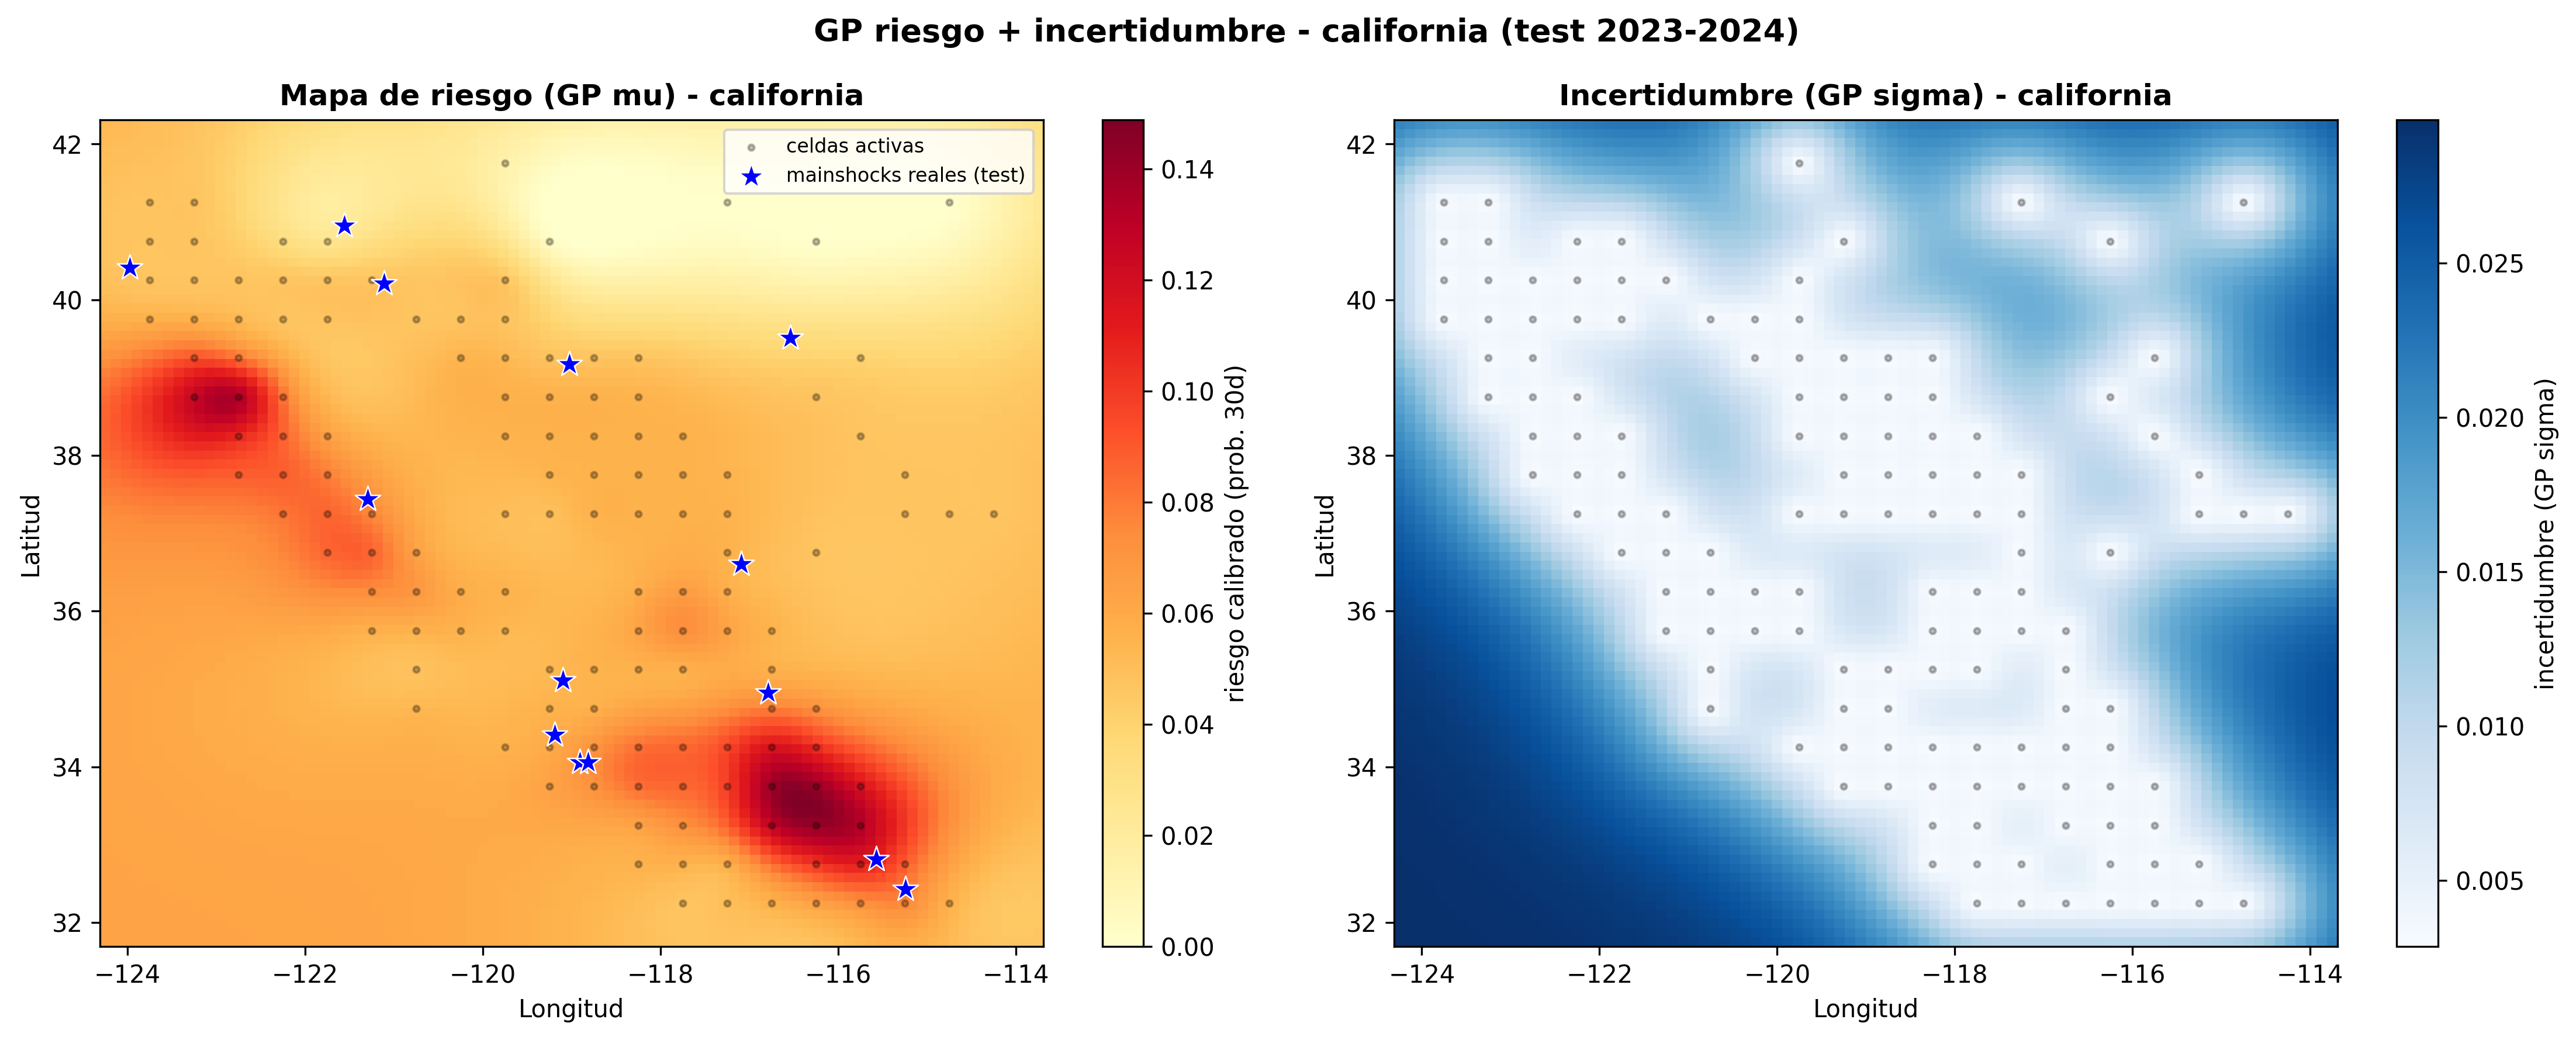
\includegraphics[width=\textwidth]{figuras/06_mapa_riesgo_gp_california}
  \caption[Mapa de riesgo e incertidumbre para California]{\textbf{Mapa de riesgo (izquierda) e incertidumbre (derecha) para California.} El riesgo se concentra a lo largo de la falla de San Andrés y sus ramales. Las estrellas marcan los mainshocks reales del periodo de test.}
  \label{fig:mapacali}
\end{figure}

\begin{figure}[ht!]
  \centering
  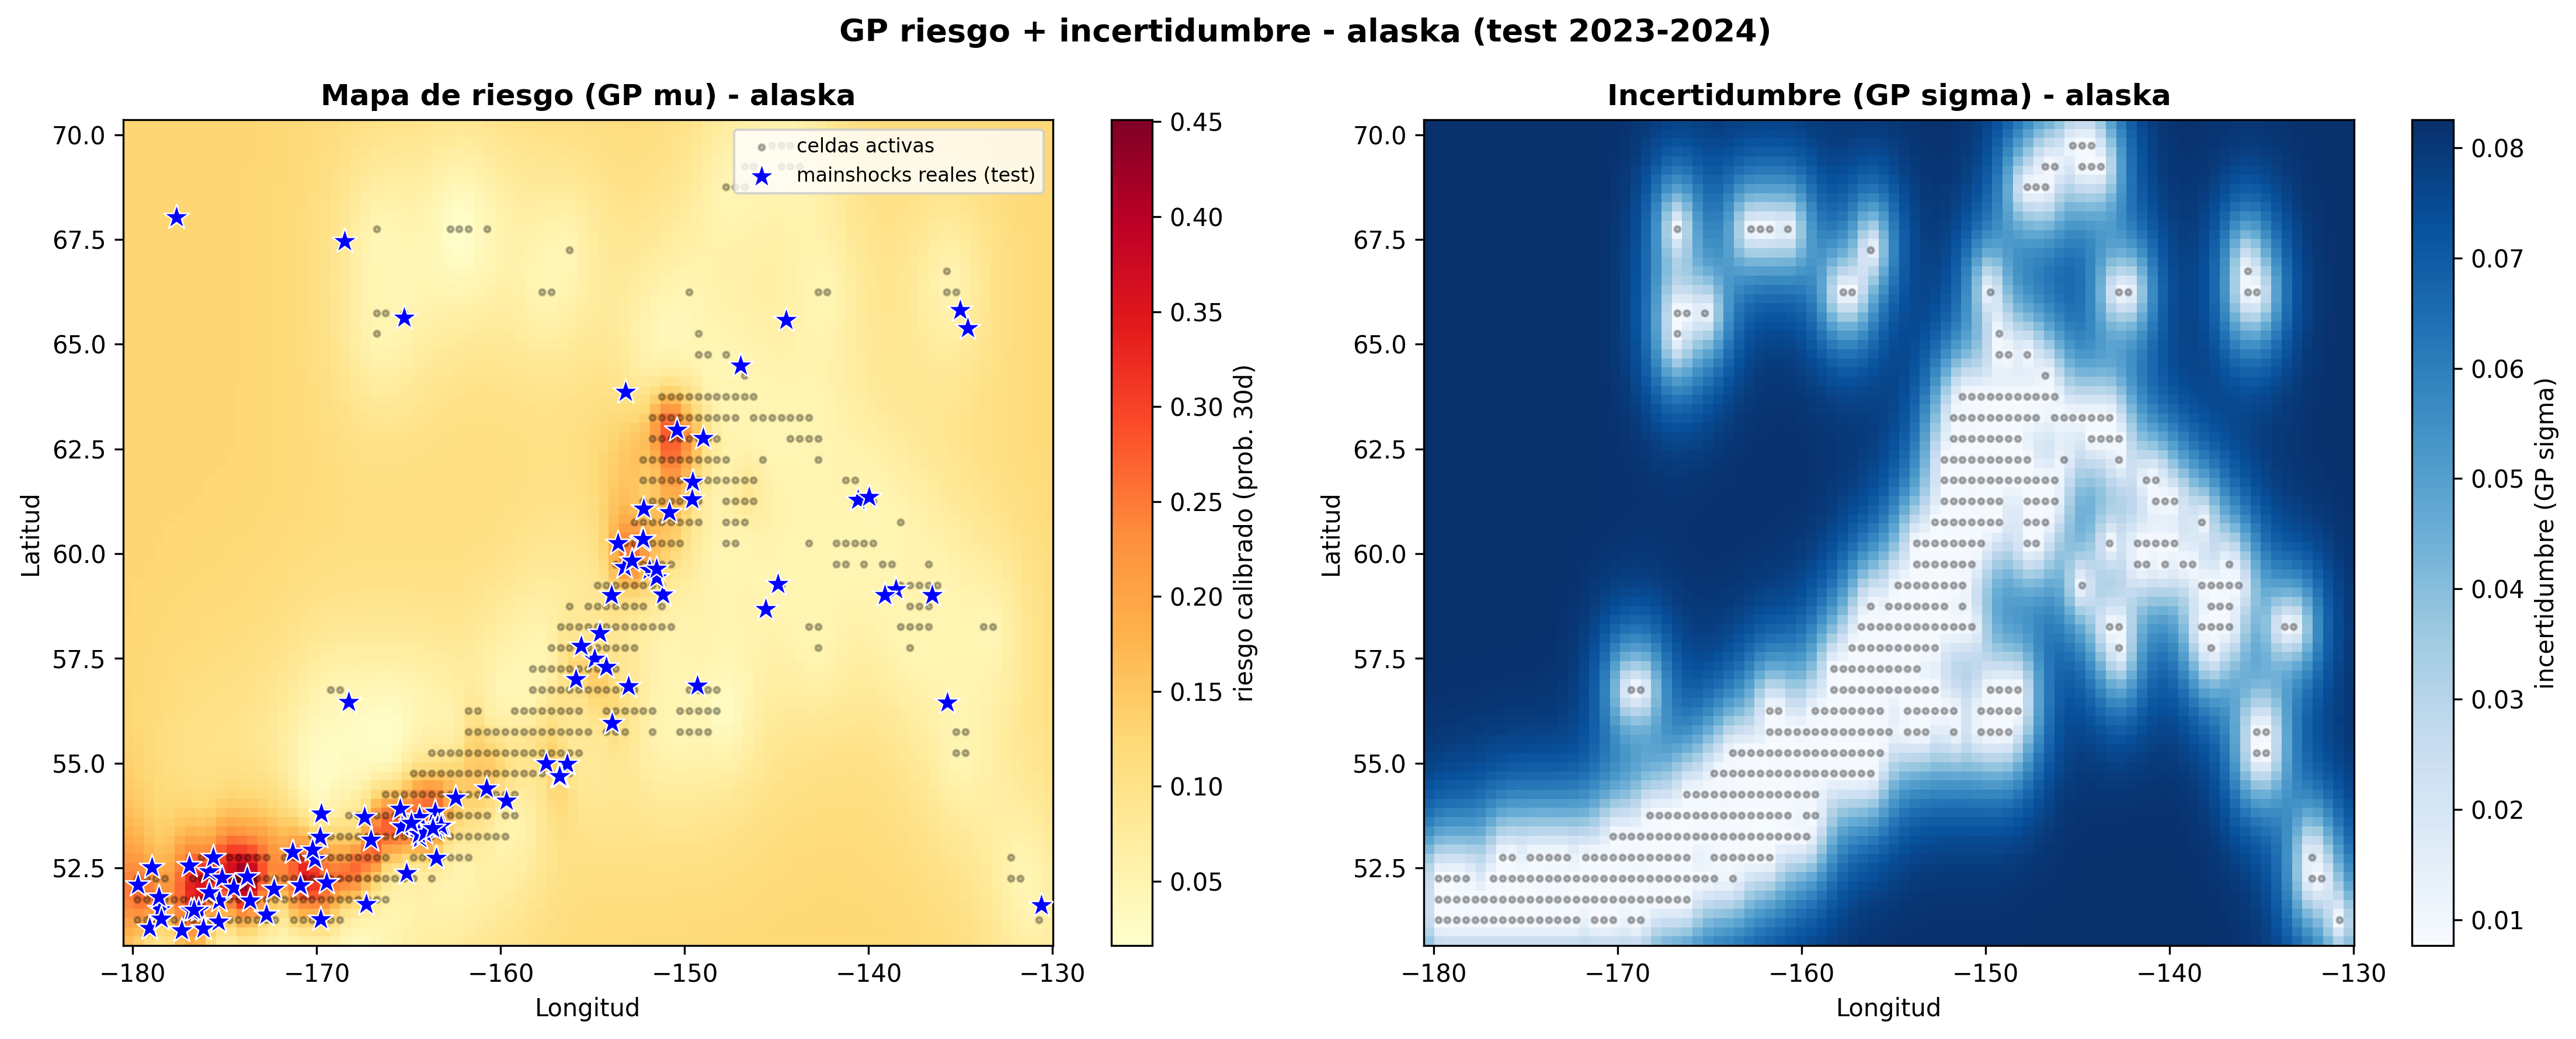
\includegraphics[width=\textwidth]{figuras/06_mapa_riesgo_gp_alaska}
  \caption[Mapa de riesgo e incertidumbre para Alaska]{\textbf{Mapa de riesgo (izquierda) e incertidumbre (derecha) para Alaska.} El riesgo se concentra en el arco de las Aleutianas y la costa sur. La incertidumbre crece en las zonas interiores sin sismicidad registrada.}
  \label{fig:mapaalaska}
\end{figure}

Para validar de forma cuantitativa la coherencia espacial del mapa se comprueba si los mainshocks
reales del test caen en las zonas de riesgo alto. El mapa distingue las celdas que registraron
mainshocks de las que no con un AUC de \textbf{0.80}, y asigna a las primeras un riesgo medio
\textbf{2.2 veces superior} al de las segundas. Esto confirma con números lo que se aprecia a
simple vista: el mapa concentra correctamente el riesgo en las zonas donde efectivamente ocurren
los terremotos.

\subsection{Generalización a otras regiones del mundo}
\label{res-transferencia}

Una pregunta natural, y muy valorada en la literatura, es si el modelo aprende algo
\emph{universal} o algo \emph{específico} de las zonas con las que se entrenó. Como el
Transformer aprende una función de las características y de la geometría --no una memoria de
celdas concretas--, en principio puede aplicarse a una región distinta sin reentrenar. Para
comprobarlo se realizó un experimento de \textbf{transferencia}: se tomó el modelo entrenado en
California+Alaska y se aplicó, \emph{en inferencia y sin reentrenar}, a nueve regiones sísmicas
de los cinco continentes (dos por continente, salvo África, donde solo el Magreb reunió datos
suficientes), replicando exactamente el mismo cálculo de características y de objetivo. Para cada
región se comparó el modelo transferido con su propia climatología de Poisson local.

\begin{table}[ht!]
  \centering
  \small
  \begin{tabular}{@{}llccccc@{}}
    \toprule
    \textbf{Región}   & \textbf{Continente} & \textbf{$M_c$} & \textbf{Celdas} & \textbf{AUC modelo} & \textbf{AUC Poisson} & \textbf{AUC temporal} \\
    \midrule
    Cascadia (PNW)    & N.\ América         & 2.8            & 31              & 0.420               & 0.809                & 0.540                 \\
    México (Guerrero) & N.\ América         & 4.0            & 64              & 0.538               & 0.600                & 0.517                 \\
    Chile norte       & S.\ América         & 4.2            & 155             & 0.511               & 0.708                & 0.511                 \\
    Perú              & S.\ América         & 4.2            & 45              & 0.479               & 0.605                & 0.541                 \\
    Italia (Apeninos) & Europa              & 2.8            & 33              & 0.441               & 0.647                & 0.556                 \\
    Grecia (Egeo)     & Europa              & 3.2            & 172             & 0.494               & 0.688                & 0.475                 \\
    Japón             & Asia                & 4.4            & 188             & \textbf{0.637}      & 0.723                & 0.465                 \\
    Sumatra           & Asia                & 4.4            & 94              & 0.545               & 0.656                & 0.552                 \\
    Magreb            & África              & 2.8            & 17              & 0.472               & 0.687                & 0.613                 \\
    \midrule
    \textbf{Media}    &                     &                &                 & \textbf{0.504}      & 0.671                & 0.530                 \\
    \bottomrule
  \end{tabular}
  \caption[Transferencia del Transformer a otras regiones]{\textbf{Transferencia del Transformer (entrenado en California+Alaska) a otras regiones.} AUC-ROC del modelo aplicado en inferencia frente a la climatología de Poisson local de cada región. En las nueve regiones el modelo queda por debajo de su climatología local, y de media su AUC (0.504) es indistinguible del azar. La AUC temporal por celda permanece próxima a 0.5, como en las regiones de entrenamiento.}
  \label{tab:transferencia}
\end{table}

La Tabla~\ref{tab:transferencia} resume el resultado. En \textbf{las nueve regiones} el modelo
transferido obtiene un AUC inferior al de la climatología local, y su valor medio, 0.504, es
\emph{indistinguible del azar}. En cinco regiones el AUC cae incluso por debajo de 0.5, lo que
indica que el orden de riesgo aprendido en California+Alaska no solo deja de ser útil, sino que
llega a ser contraproducente fuera de su dominio. La AUC temporal por celda se mantiene en torno
a 0.5, igual que en casa. Es decir, el modelo \textbf{no generaliza}: el mapa espacial de peligro
que captura es específico de las zonas con las que se entrenó.

Este resultado, lejos de ser un inconveniente, delimita con precisión el alcance del sistema y
admite una lectura \textbf{tectónica} coherente. Las regiones donde el modelo transfiere
\emph{menos mal} son Japón (0.637) y Sumatra (0.545), que elevan la media de Asia (0.591) por
encima de la del resto de continentes (entre 0.47 y 0.50). Ambas son
\textbf{zonas de subducción muy activas} --el mismo régimen tectónico que Alaska, una de las dos
regiones de entrenamiento-- en las que la sismicidad se alinea de forma marcada a lo largo de la
fosa. Esa estructura espacial intensa y bien definida es la que el mecanismo de atención puede
aprovechar parcialmente, aun aplicado fuera de su dominio. En el extremo opuesto, las regiones
donde peor transfiere son Cascadia (0.420), una zona de subducción \emph{bloqueada} y
sísmicamente tranquila en su interfaz, e Italia (0.441), de tectónica extensional difusa: en
ambas la geometría de la sismicidad se parece poco a la de California o Alaska. Las zonas de
subducción de Sudamérica (Chile, Perú) y de México quedan en una posición intermedia, penalizadas
además por una magnitud de completitud alta (en torno a $M_c \approx 4$) que empobrece sus
características. Conviene subrayar que ni siquiera Japón, la región más favorable, supera a su
climatología local: la similitud tectónica con Alaska ayuda, pero no basta para reconstruir el
mapa de peligro específico de otra región. En conjunto, el experimento confirma de forma directa
el hallazgo central del trabajo: el valor del sistema está en cartografiar la estructura
\emph{espacial} del peligro allí donde se entrena, y esa estructura es propia de cada región.

\subsection{Discusión de los resultados en el contexto del estado del arte}
\label{res-discusion}

Conviene situar los resultados anteriores en el marco de lo que la comunidad sismológica
considera alcanzable. El pronóstico de terremotos a corto plazo es, posiblemente, uno de los
problemas abiertos más difíciles de la geofísica, y la postura mayoritaria es que no existe un
método capaz de anticipar de forma fiable el instante de un sismo concreto con semanas de
antelación \citep{geller1997unpredictable, jordan2011oef}. Los sistemas operacionales más consolidados, como los basados en modelos de tipo
ETAS, no predicen tanto el \emph{momento} de un evento aislado como la \emph{tasa esperada} de
sismicidad, que aumenta tras un terremoto grande por el efecto de las réplicas \citep{ogata1988etas, marzocchi2014oef}. En ese contexto,
los resultados de este trabajo encajan de forma natural y coherente.

El primer punto de contacto es el papel de la climatología. En la evaluación de pronósticos
sísmicos es habitual que el listón a batir sea un modelo de tasa de fondo, precisamente porque
una parte muy grande de la ``predictibilidad'' de los terremotos se reduce a saber qué zonas son
crónicamente activas \citep{helmstetter2006comparison}. Que el Transformer iguale y supere ligeramente a la climatología de
Poisson, de forma estadísticamente significativa, es un resultado sólido: muchos métodos
sofisticados de la literatura no consiguen batir esta referencia de manera consistente
\citep{zechar2008testing, beroza2021dlreview}. Un caso ilustrativo es el de
\citet{devries2018aftershocks}, cuya red profunda para la predicción espacial de réplicas fue
posteriormente igualada por un \textit{baseline} de una sola neurona \citep{mignan2019oneneuron}. El
sistema, por tanto, se sitúa en el lado correcto de esa frontera.

El segundo punto, y el más importante, es la localización de la señal. El análisis con la AUC
temporal por celda muestra que la capacidad del sistema reside en la dimensión espacial y no en
la temporal a 30 días. Esta conclusión está en plena sintonía con el consenso científico: la
acumulación de tensión tectónica que conduce a un terremoto se desarrolla a lo largo de años y
de forma silenciosa \citep{stein2003introduction}, por lo que es razonable que un catálogo de eventos discretos no contenga la
firma precursora del momento exacto. Lo relevante de este trabajo no es, por tanto, ``descubrir''
que el pronóstico temporal es difícil --algo bien sabido-- sino \emph{medirlo con una métrica
  limpia} que separa ambas dimensiones, evitando la confusión, frecuente en la literatura aplicada,
entre acertar dónde y acertar cuándo. Un AUC global de 0.73 podría presentarse, sin este
análisis, como una capacidad de pronóstico temporal que en realidad no existe.

El tercer punto es la comparación entre arquitecturas. El hecho de que la GNN y el Transformer
--dos formas muy distintas de modelar el espacio-- lleguen esencialmente a la misma conclusión
refuerza su validez: no se trata de un artefacto de un diseño concreto, sino de una propiedad del
problema y de los datos. Esta convergencia entre métodos independientes es justamente el tipo de
evidencia que da credibilidad a un hallazgo.

El cuarto punto lo aporta el experimento de transferencia (Sección~\ref{res-transferencia}). Que
el modelo no generalice a otras regiones encaja con lo que cabe esperar de un sistema que, según
el análisis anterior, aprende fundamentalmente un \emph{mapa espacial de peligro}: dado que la
geometría de la sismicidad es propia de cada contexto tectónico, un mapa ajustado a la falla de
San Andrés y al arco de las Aleutianas no tiene por qué servir para la subducción andina o la
extensión del Egeo. La lectura tectónica de los resultados --el modelo transfiere algo mejor a las
subducciones muy activas de Asia, parecidas a Alaska, y peor a las zonas de geometría difusa o
tranquila-- es coherente con esta interpretación y, a la vez, marca el camino para mejorar: la
generalización exigiría reentrenar con datos de cada región o emplear técnicas de adaptación de
dominio, un problema bien documentado al transferir modelos profundos en sismología entre
conjuntos de datos y regiones distintas \citep{munchmeyer2022picker}. En conjunto, los resultados no solo son compatibles con el estado del arte, sino que
aportan una forma más honesta y precisa de evaluar este tipo de sistemas --separando el dónde del
cuándo y midiendo explícitamente la transferibilidad-- que es una contribución metodológica de
valor más allá del caso concreto estudiado.

\subsection{Síntesis de los resultados}
\label{res-sintesis}

En conjunto, los resultados dibujan un sistema que cumple su objetivo de extremo a extremo. La
detección funciona con alta fidelidad; los modelos espaciales capturan con éxito la estructura del
peligro sísmico y el mejor de ellos, el Transformer, supera de forma significativa a la
climatología; las métricas operativas confirman una capacidad de alerta cuatro veces superior al
azar; y el proceso gaussiano produce mapas de riesgo calibrados y acompañados de incertidumbre. El
análisis de la dimensión temporal, mediante una métrica diseñada al efecto, localiza con precisión
la información predictiva en la componente espacial y muestra que el horizonte temporal de 30 días
sobre el catálogo no aporta señal adicional, un resultado riguroso y alineado con el estado del
arte. El experimento de transferencia a nueve regiones de los cinco continentes completa el
diagnóstico: el sistema no generaliza fuera de su dominio de entrenamiento, lo que confirma que su
capacidad consiste en cartografiar la estructura espacial del peligro, propia de cada región, y no
en un patrón universal. El siguiente capítulo interpreta estos hallazgos a la luz de los objetivos
planteados.
